%
\begin{isabellebody}%
\def\isabellecontext{AbstractObjects}%
%
\isadelimtheory
%
\endisadelimtheory
%
\isatagtheory
%
\endisatagtheory
{\isafoldtheory}%
%
\isadelimtheory
%
\endisadelimtheory
%
\isamarkupsection{Introduction%
}
\isamarkuptrue%
%
\begin{isamarkuptext}%
The Isabelle/HOL formalisation presented in this article is related to the ongoing 
  Principia Metaphysica \cite{zalta:_princ_metap} project at Stanford University.
  This project, which exploits and extends Zalta's  Theory of Abstract 
  Objects \cite{zalta83:_abstr_objec}, 
  employs a modal relational type theory (MRTT) as logical foundation. Arguments
  defending this choice against a modal functional type theory (MFTT)
  have been presented before \cite{zalta11:_relat_versus_funct_found_logic}.
  In a nutshell, the situation is this: functional type theory comes with strong 
  comprehension principles, which, in the context of the Theory of Abstract Objects, 
  have paradoxical implications. When starting off with a relational foundation, however, 
  weaker comprehension principles are provided, and these obstacles can be avoided.

  Isabelle/HOL is a proof assistant based on a functional type theory extending
  Church's theory of types \cite{Church40}, and recently it has been shown 
  that Church's type theory can be elegantly utilized as a meta-logic to encode and 
  automate various quantified non-classical logics, including MFTT \cite{J23,C40}. 
  This work has subsequently been employed in a case study in
  computational metaphysics, in which different variants of Kurt Gödel's ontological 
  argument were verified resp. falsified \cite{C40,C55}. 
 

  The motivating research questions for the formalisation presented below include:
  \begin{itemize} 
  \item Can functional type theory, despite the problems pointed at by Zalta and Oppenheimer, 
   also be utilized to encode MRTT and subsequently the Theory of Abstract Objects when 
   following the embeddings approach?
  \item How elegant and user-friendly is the resulting formalization? 
   To what extend can Isabelle's  user interface be facilitated to hide 
   unpleasant technicalities of the (extended) embedding from the user?
  \item How far can automation be pushed in the approach to minimise user interaction  in the 
    formalization of the Theory of Abstract objects? 
  \item Can the consistency of the theory eventually be validated with the available automated 
   reasoning tools?
  \item Can the reasoners eventually even contribute some new knowledge? 
  \item Are any suggestions for improvements in Isabelle arising? 
   What are the particular problems detected in the course of the study?
  \end{itemize}

  In this contribution to the Archive of Formal Proofs we focus on the encoding 
  of MRTT in functional type theory. The idea is to reuse and adapt the fundamental ideas underlying
  the previous encoding of MFTT in functional type theory \cite{J23,C40}, which has been realised 
  inter alia in Isabelle/HOL \cite{J28}. In subsequent work we will then reuse and extend the 
  foundations provided in this article.
 
  The encoding of modal functional type theory in functional type theory as explored in 
  previous work  is simple: modal logic formulas are identified with certain functional 
  type theory formulas of predicate type \isa{i{\isasymRightarrow}bool} (abbreviated as \isa{io} below). 
  Possible worlds are explicitly represented by 
  terms of type  \isa{i}. A modal logic formula \isa{{\isasymphi}} holds for a world \isa{w} if and 
  only if the application \isa{{\isasymphi}\ w} evaluates to true. The definition of the propositional modal logic 
  connectives is then straightforward and it simply realizes the standard translation as a set of equations 
  in functional type theory. The approach has been successfully extended for quantifiers. A crucial 
  aspect thereby is that in simple type theory quantifiers can be treated
  as ordinary logical connectives. No extra binding mechanism is needed since the already existing 
  lambda binding mechanism can be elegantly utilized. 
  
  The challenge for this work has been to suitably appropriately 'restrict' this embedding for modal relational type theory.
  The grammar of modal relational type theory is presented in Figure~\ref{mmrt}.
   \begin{figure}[t]
  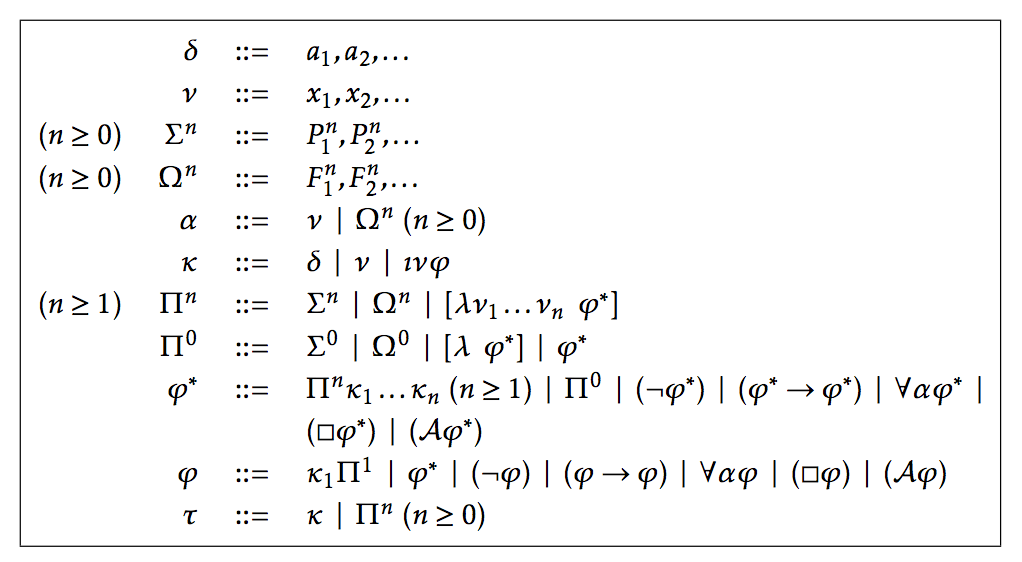
\includegraphics[height=5.5cm]{ModalRelationalTypeTheory.png}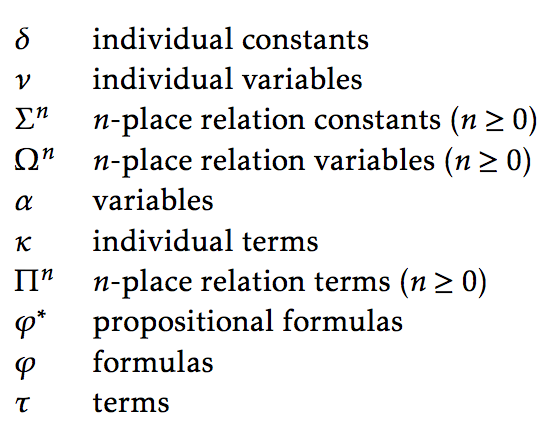
\includegraphics[height=4.5cm]{ModalRelationalTypeTheory2.png}
  \caption{Grammar of MRTT, cf. \cite{zalta:_princ_metap} for further details in MRTT. \label{mmrt}
  Two kinds of (complex) formulas are introduced: ones that may have encoding subformulas and 
  ones that do not. The latter are designated as propositional formulas, the former ones simply as formulas.}
  \end{figure}
  Note that this grammar excludes terms such as $\lambda x. Rx \rightarrow xR$, where $Rx$ represents the 
  exemplification of property $R$ by $x$ and $xR$ stands for the encoding of property $R$ by $x$. The reason is 
  that such kind of  
  lambda-abstractions may lead to paradoxes in the theory of abstract 
  objects \cite{zalta11:_relat_versus_funct_found_logic}.
  

  To achieve our goal we provide means to explicitly represents and propagate information  on the 
  syntactical structure of MRTT in functional type theory. In particular, we provide means in form of annotations 
  to explicitly distinguish 
  between propositional formulas, formulas, terms and erroneous (ineligible/excluded) formations. 
  Respective annotation information is propagated from the innermost constituents to the top level constructions.
  This clearly creates some significant technical overhead. However, we fruitfully exploit facilities in Isabelle/HOL's user 
  interface, and other means, to hide most of these technicalities from the user in applications.

  A note on using abbreviations versus definitions in our approach:  We are aware that abbreviations should
  be used sparsingly in Isabelle/HOL, since they are automatically expanded and thus lead to a discrepancy 
  between the internal and the external view of a term. However, here we deliberately deviate from this
  rule, since one aspect of the paper is to exactly illustrate this discrepancy and to emphasize the complexity
  of the embedding MRTT in functional type theory. In fact, this complexity makes pen and paper 
  work with the proposed embedding pragmatically infeasible, as we believe, while in a proof assistant like 
   Isabelle/HOL
  in can, at least to some degree, still be handled by an interactive user. Moreover, as we will also
  illustrate, the simplifier \isa{simp} of Isabelle/HOL is well capable of effectively reducing
  this complexity again. In other words, the simplifier effectievely analyses and and rewrites the 
  deeply annotated terms and propagates the annotation information to the top-level only as intended.
  It is exactly this effect which we want to illustrate and exploit here.\footnote{We have also 
  experimented with the alternative use of definitions; the respective 
  encodings can be requested from the authors.}%
\end{isamarkuptext}%
\isamarkuptrue%
%
\isamarkupsection{Preliminaries%
}
\isamarkuptrue%
%
\begin{isamarkuptext}%
We start out with some type declarations and type abbreviations. 
  Our formalism explicitly encodes possible world semantics. Hence, we introduce a 
  distinguished type \isa{i} to represent the set of possible worlds. 
  Consequently, terms of this type denote possible worlds. 
  Moreover, modal logic formulas are associated in our approach with
  predicates (resp. sets) on possible worlds. Hence, modal logic formulas have
  type \isa{{\isacharparenleft}i\ {\isasymRightarrow}\ bool{\isacharparenright}}. To make our representation  more concise in the remainder
  we abbreviate this type as \isa{io}.%
\end{isamarkuptext}%
\isamarkuptrue%
\ \isacommand{typedecl}\isamarkupfalse%
\ i\isanewline
\ \isacommand{type{\isacharunderscore}synonym}\isamarkupfalse%
\ io\ {\isacharequal}\ {\isachardoublequoteopen}{\isacharparenleft}i\ {\isasymRightarrow}\ bool{\isacharparenright}{\isachardoublequoteclose}%
\begin{isamarkuptext}%
Entities in the abstract theory of types are represented in our formalism by the
  type \isa{e}. We call this the raw type of entities resp. objects. The Theory of Abstract Objects 
  later introduces means to distinguish between abstract and ordinary entities.%
\end{isamarkuptext}%
\isamarkuptrue%
\ \isacommand{typedecl}\isamarkupfalse%
\ e%
\begin{isamarkuptext}%
To explicitly model the syntactical restrictions of MRTT we introduce a 
  (polymorphic) datatype \isa{{\isacharprime}a\ opt} (\isa{{\isacharprime}a} is a type variable) 
  based on four constructors: \isa{ERR\ {\isacharprime}a} (identifies ineligible/excluded constructions), \isa{P\ {\isacharprime}a} 
  (identifies propositional formulas), \isa{F\ {\isacharprime}a} (identifies  formulas), and \isa{T\ {\isacharprime}a} (identifies 
  eligible terms, such as lambda abstractions). The embeddings approach (of MFTT in functional type theory)
  will be suitably adapted below so that 
  for each language expression (in the embedded MRTT) the respective datatype 
  is identified and appropriately propagated. The encapsulated expressions  
  then correspond to the previous embedding of MRTT in  functional type theory.%
\end{isamarkuptext}%
\isamarkuptrue%
\ \isacommand{datatype}\isamarkupfalse%
\ {\isacharprime}a\ opt\ {\isacharequal}\ ERR\ {\isacharprime}a\ {\isacharbar}\ P\ {\isacharprime}a\ {\isacharbar}\ F\ {\isacharprime}a\ {\isacharbar}\ T\ {\isacharprime}a%
\begin{isamarkuptext}%
The following operators support a concise and elegant superscript annotation with these
  four syntactical categories for our language constructs.%
\end{isamarkuptext}%
\isamarkuptrue%
\ \isacommand{abbreviation}\isamarkupfalse%
\ mkP{\isacharcolon}{\isacharcolon}{\isachardoublequoteopen}io{\isasymRightarrow}io\ opt{\isachardoublequoteclose}\ {\isacharparenleft}{\isachardoublequoteopen}{\isacharunderscore}\isactrlsup P{\isachardoublequoteclose}\ {\isacharbrackleft}{\isadigit{1}}{\isadigit{0}}{\isadigit{9}}{\isacharbrackright}\ {\isadigit{1}}{\isadigit{1}}{\isadigit{0}}{\isacharparenright}\ \ \isakeyword{where}\ {\isachardoublequoteopen}{\isasymphi}\isactrlsup P\ {\isasymequiv}\ P\ {\isasymphi}{\isachardoublequoteclose}\ \isanewline
\ \isacommand{abbreviation}\isamarkupfalse%
\ mkF{\isacharcolon}{\isacharcolon}{\isachardoublequoteopen}io{\isasymRightarrow}io\ opt{\isachardoublequoteclose}\ {\isacharparenleft}{\isachardoublequoteopen}{\isacharunderscore}\isactrlsup F{\isachardoublequoteclose}\ {\isacharbrackleft}{\isadigit{1}}{\isadigit{0}}{\isadigit{9}}{\isacharbrackright}\ {\isadigit{1}}{\isadigit{1}}{\isadigit{0}}{\isacharparenright}\ \ \isakeyword{where}\ {\isachardoublequoteopen}{\isasymphi}\isactrlsup F\ {\isasymequiv}\ F\ {\isasymphi}{\isachardoublequoteclose}\ \isanewline
\ \isacommand{abbreviation}\isamarkupfalse%
\ mkT{\isacharcolon}{\isacharcolon}{\isachardoublequoteopen}{\isacharprime}a{\isasymRightarrow}{\isacharprime}a\ opt{\isachardoublequoteclose}\ {\isacharparenleft}{\isachardoublequoteopen}{\isacharunderscore}\isactrlsup T{\isachardoublequoteclose}\ {\isacharbrackleft}{\isadigit{1}}{\isadigit{0}}{\isadigit{9}}{\isacharbrackright}\ {\isadigit{1}}{\isadigit{1}}{\isadigit{0}}{\isacharparenright}\ \ \isakeyword{where}\ {\isachardoublequoteopen}{\isasymphi}\isactrlsup T\ {\isasymequiv}\ T\ {\isasymphi}{\isachardoublequoteclose}\isanewline
\ \isacommand{abbreviation}\isamarkupfalse%
\ mkE{\isacharcolon}{\isacharcolon}{\isachardoublequoteopen}{\isacharprime}a{\isasymRightarrow}{\isacharprime}a\ opt{\isachardoublequoteclose}\ {\isacharparenleft}{\isachardoublequoteopen}{\isacharunderscore}\isactrlsup E{\isachardoublequoteclose}\ {\isacharbrackleft}{\isadigit{1}}{\isadigit{0}}{\isadigit{9}}{\isacharbrackright}\ {\isadigit{1}}{\isadigit{1}}{\isadigit{0}}{\isacharparenright}\ \ \isakeyword{where}\ {\isachardoublequoteopen}{\isasymphi}\isactrlsup E\ {\isasymequiv}\ ERR\ {\isasymphi}{\isachardoublequoteclose}%
\begin{isamarkuptext}%
Certain language constructs in the Theory of Abstract objects, such as the actuality operator  
  \isa{\isactrlbold {\isasymA}} ("it is actually the case that"), refer to a (fixed) designated world. To model such a 
  rigid dependence we introduce a constant symbol (name) \isa{dw} of world type \isa{i}. 
  Moreover, for technical reasons, 
  which will be clarified below, we introduce further (dummy) constant symbols for the various other domains. Since
  we anyway assume that all domains are non-empty, introducing these constant symbols is obviously not harmful. 
  \footnote{The single polymorphic dummy \isa{\isactrlbold da{\isacharcolon}{\isacharcolon}{\isacharprime}a}, utilized e.g. in the definition of the universal 
  quantifier of MRTT below, would actually cover all cases. However, to avoid type inference we
  actually prefer non-polymorphic dummy elements in all those cases where we can statically 
  predetermine the required type.}%
\end{isamarkuptext}%
\isamarkuptrue%
\ \isacommand{consts}\isamarkupfalse%
\ dw\ {\isacharcolon}{\isacharcolon}\ i\ \isanewline
\ \isacommand{consts}\isamarkupfalse%
\ de{\isacharcolon}{\isacharcolon}{\isachardoublequoteopen}e{\isachardoublequoteclose}\ dio{\isacharcolon}{\isacharcolon}{\isachardoublequoteopen}io{\isachardoublequoteclose}\ deio{\isacharcolon}{\isacharcolon}{\isachardoublequoteopen}e{\isasymRightarrow}io{\isachardoublequoteclose}\ da{\isacharcolon}{\isacharcolon}{\isacharprime}a%
\isamarkupsection{Embedding of Modal Relational Type Theory%
}
\isamarkuptrue%
%
\begin{isamarkuptext}%
The various language constructs of MRTT (see Figure \ref{mmrt}) are now introduced step by step.%
\end{isamarkuptext}%
\isamarkuptrue%
%
\begin{isamarkuptext}%
The actuality operator \isa{\isactrlbold {\isasymA}}, when being applied to a formula or propositional formula 
  \isa{{\isasymphi}}, evaluates \isa{{\isasymphi}} wrt the fixed given world \isa{dw}. 
  The compound expression \isa{\isactrlbold {\isasymA}{\isasymphi}} inherits its syntactical category  \isa{F} (formula) or
  \isa{P} (propositional formula from \isa{{\isasymphi}}. If the syntactical catagory of  \isa{{\isasymphi}} is 
  \isa{ERR} (error) or \isa{T} (term), then the syntactical catagory of \isa{\isactrlbold {\isasymA}{\isasymphi}} 
  is \isa{ERR} and a dummy entity of appropriate type is returned. This illustrates the core 
  ideas of our explicit modeling of MRTT grammatical structure in functional type theory. 
  This scheme will repeated below for all the other language constructs of MRTT.%
\end{isamarkuptext}%
\isamarkuptrue%
\ \isacommand{abbreviation}\isamarkupfalse%
\ Actual{\isacharcolon}{\isacharcolon}{\isachardoublequoteopen}io\ opt\ {\isasymRightarrow}\ io\ opt{\isachardoublequoteclose}\ {\isacharparenleft}{\isachardoublequoteopen}\isactrlbold {\isasymA}\ {\isacharunderscore}{\isachardoublequoteclose}\ {\isacharbrackleft}{\isadigit{6}}{\isadigit{4}}{\isacharbrackright}\ {\isadigit{6}}{\isadigit{5}}{\isacharparenright}\ \isakeyword{where}\ {\isachardoublequoteopen}\isactrlbold {\isasymA}{\isasymphi}\ {\isasymequiv}\ case\ {\isasymphi}\ of\ \isanewline
\ \ \ \ F{\isacharparenleft}{\isasympsi}{\isacharparenright}\ {\isasymRightarrow}\ F{\isacharparenleft}{\isasymlambda}w{\isachardot}\ {\isasympsi}\ dw{\isacharparenright}\ {\isacharbar}\ P{\isacharparenleft}{\isasympsi}{\isacharparenright}\ {\isasymRightarrow}\ P{\isacharparenleft}{\isasymlambda}w{\isachardot}\ {\isasympsi}\ dw{\isacharparenright}\ {\isacharbar}\ {\isacharunderscore}\ {\isasymRightarrow}\ ERR{\isacharparenleft}dio{\isacharparenright}{\isachardoublequoteclose}%
\begin{isamarkuptext}%
The Theory of Abstract Objects distinguishes between encoding properties \isa{{\isasymkappa}\isactrlsub {\isadigit{1}}{\isasymPi}\isactrlsup {\isadigit{1}}} and 
  exemplifying properties \isa{{\isasymPi}\isactrlsup n{\isacharcomma}{\isasymkappa}\isactrlsub {\isadigit{1}}{\isacharcomma}{\isachardot}{\isachardot}{\isacharcomma}{\isasymkappa}\isactrlsub n} (for $n\geq 1$). 

  Encoding \isa{{\isasymkappa}\isactrlsub {\isadigit{1}}{\isasymPi}\isactrlsup {\isadigit{1}}} is noted below as \isa{{\isasymlbrace}{\isasymkappa}\isactrlsub {\isadigit{1}}{\isacharcomma}{\isasymPi}\isactrlsup {\isadigit{1}}{\isasymrbrace}}.
  Encoding yields formulas and never propositional formulas. It is mapped to predicate application.%
\end{isamarkuptext}%
\isamarkuptrue%
\ \isacommand{abbreviation}\isamarkupfalse%
\ Enc{\isacharcolon}{\isacharcolon}{\isachardoublequoteopen}e\ opt{\isasymRightarrow}{\isacharparenleft}e{\isasymRightarrow}io{\isacharparenright}\ opt{\isasymRightarrow}io\ opt{\isachardoublequoteclose}\ {\isacharparenleft}{\isachardoublequoteopen}{\isasymlbrace}{\isacharunderscore}{\isacharcomma}{\isacharunderscore}{\isasymrbrace}{\isachardoublequoteclose}{\isacharparenright}\ \isakeyword{where}\ {\isachardoublequoteopen}{\isasymlbrace}x{\isacharcomma}{\isasymPhi}{\isasymrbrace}\ {\isasymequiv}\ case\ {\isacharparenleft}x{\isacharcomma}{\isasymPhi}{\isacharparenright}\ of\ \isanewline
\ \ \ \ {\isacharparenleft}T{\isacharparenleft}y{\isacharparenright}{\isacharcomma}T{\isacharparenleft}Q{\isacharparenright}{\isacharparenright}\ {\isasymRightarrow}\ F{\isacharparenleft}Q\ y{\isacharparenright}\ {\isacharbar}\ {\isacharunderscore}\ {\isasymRightarrow}\ ERR{\isacharparenleft}dio{\isacharparenright}{\isachardoublequoteclose}%
\begin{isamarkuptext}%
Unary exemplifying formulas \isa{{\isasymPi}\isactrlsup {\isadigit{1}}{\isasymkappa}\isactrlsub {\isadigit{1}}} are noted below as \isa{{\isasymlparr}{\isasymPi}\isactrlsup {\isadigit{1}}{\isacharcomma}{\isasymkappa}\isactrlsub {\isadigit{1}}{\isasymrparr}}.  
  Exemplification yields propositional formulas. Like encoding, it is then mapped to predicate application.%
\end{isamarkuptext}%
\isamarkuptrue%
\ \isacommand{abbreviation}\isamarkupfalse%
\ Exe{\isadigit{1}}{\isacharcolon}{\isacharcolon}{\isachardoublequoteopen}{\isacharparenleft}e{\isasymRightarrow}io{\isacharparenright}\ opt{\isasymRightarrow}e\ opt{\isasymRightarrow}io\ opt{\isachardoublequoteclose}\ {\isacharparenleft}{\isachardoublequoteopen}{\isasymlparr}{\isacharunderscore}{\isacharcomma}{\isacharunderscore}{\isasymrparr}{\isachardoublequoteclose}{\isacharparenright}\ \isakeyword{where}\ {\isachardoublequoteopen}{\isasymlparr}{\isasymPhi}{\isacharcomma}x{\isasymrparr}\ {\isasymequiv}\ case\ {\isacharparenleft}{\isasymPhi}{\isacharcomma}x{\isacharparenright}\ of\ \isanewline
\ \ \ \ {\isacharparenleft}T{\isacharparenleft}Q{\isacharparenright}{\isacharcomma}T{\isacharparenleft}y{\isacharparenright}{\isacharparenright}\ {\isasymRightarrow}\ P{\isacharparenleft}Q\ y{\isacharparenright}\ {\isacharbar}\ {\isacharunderscore}\ {\isasymRightarrow}\ ERR{\isacharparenleft}dio{\isacharparenright}{\isachardoublequoteclose}%
\begin{isamarkuptext}%
For pragmatical reasons we support exemplification formulas \isa{{\isasymPi}\isactrlsup n{\isacharcomma}{\isasymkappa}\isactrlsub {\isadigit{1}}{\isacharcomma}{\isachardot}{\isachardot}{\isacharcomma}{\isasymkappa}\isactrlsub n} here only for \isa{{\isadigit{1}}{\isasymle}n{\isasymle}{\isadigit{3}}}.
 In addition to the unary case above, we thus introduce two further cases.%
\end{isamarkuptext}%
\isamarkuptrue%
\ \isacommand{abbreviation}\isamarkupfalse%
\ Exe{\isadigit{2}}{\isacharcolon}{\isacharcolon}{\isachardoublequoteopen}{\isacharparenleft}e{\isasymRightarrow}e{\isasymRightarrow}io{\isacharparenright}\ opt{\isasymRightarrow}e\ opt{\isasymRightarrow}e\ opt{\isasymRightarrow}io\ opt{\isachardoublequoteclose}\ {\isacharparenleft}{\isachardoublequoteopen}{\isasymlparr}{\isacharunderscore}{\isacharcomma}{\isacharunderscore}{\isacharcomma}{\isacharunderscore}{\isasymrparr}{\isachardoublequoteclose}{\isacharparenright}\isanewline
\ \ \isakeyword{where}\ {\isachardoublequoteopen}{\isasymlparr}{\isasymPhi}{\isacharcomma}x{\isadigit{1}}{\isacharcomma}x{\isadigit{2}}{\isasymrparr}\ {\isasymequiv}\ case\ {\isacharparenleft}{\isasymPhi}{\isacharcomma}x{\isadigit{1}}{\isacharcomma}x{\isadigit{2}}{\isacharparenright}\ of\ \isanewline
\ \ \ \ {\isacharparenleft}T{\isacharparenleft}Q{\isacharparenright}{\isacharcomma}T{\isacharparenleft}y{\isadigit{1}}{\isacharparenright}{\isacharcomma}T{\isacharparenleft}y{\isadigit{2}}{\isacharparenright}{\isacharparenright}\ {\isasymRightarrow}\ P{\isacharparenleft}Q\ y{\isadigit{1}}\ y{\isadigit{2}}{\isacharparenright}\ {\isacharbar}\ {\isacharunderscore}\ {\isasymRightarrow}\ ERR{\isacharparenleft}dio{\isacharparenright}{\isachardoublequoteclose}\isanewline
\ \isacommand{abbreviation}\isamarkupfalse%
\ Exe{\isadigit{3}}{\isacharcolon}{\isacharcolon}{\isachardoublequoteopen}{\isacharparenleft}e{\isasymRightarrow}e{\isasymRightarrow}e{\isasymRightarrow}io{\isacharparenright}\ opt{\isasymRightarrow}e\ opt{\isasymRightarrow}e\ opt{\isasymRightarrow}e\ opt{\isasymRightarrow}io\ opt{\isachardoublequoteclose}\ {\isacharparenleft}{\isachardoublequoteopen}{\isasymlparr}{\isacharunderscore}{\isacharcomma}{\isacharunderscore}{\isacharcomma}{\isacharunderscore}{\isacharcomma}{\isacharunderscore}{\isasymrparr}{\isachardoublequoteclose}{\isacharparenright}\ \isanewline
\ \ \isakeyword{where}\ {\isachardoublequoteopen}{\isasymlparr}{\isasymPhi}{\isacharcomma}x{\isadigit{1}}{\isacharcomma}x{\isadigit{2}}{\isacharcomma}x{\isadigit{3}}{\isasymrparr}\ {\isasymequiv}\ case\ {\isacharparenleft}{\isasymPhi}{\isacharcomma}x{\isadigit{1}}{\isacharcomma}x{\isadigit{2}}{\isacharcomma}x{\isadigit{3}}{\isacharparenright}\ of\ \isanewline
\ \ \ \ {\isacharparenleft}T{\isacharparenleft}Q{\isacharparenright}{\isacharcomma}T{\isacharparenleft}y{\isadigit{1}}{\isacharparenright}{\isacharcomma}T{\isacharparenleft}y{\isadigit{2}}{\isacharparenright}{\isacharcomma}T{\isacharparenleft}y{\isadigit{3}}{\isacharparenright}{\isacharparenright}\ {\isasymRightarrow}\ P{\isacharparenleft}Q\ y{\isadigit{1}}\ y{\isadigit{2}}\ y{\isadigit{3}}{\isacharparenright}\ {\isacharbar}\ {\isacharunderscore}\ {\isasymRightarrow}\ ERR{\isacharparenleft}dio{\isacharparenright}{\isachardoublequoteclose}%
\begin{isamarkuptext}%
Formations with negation and implication are supported for both, formulas and propositional
  formulas, and their embeddings are straightforward. In the case of implication, the compound formula
  is a propositional formula if both constituents are propositional formulas. If at least one constituent 
  is a formula and the other one eligible, then the compound formula is a formula. In all other
  cases an ERR-Formula is returned.%
\end{isamarkuptext}%
\isamarkuptrue%
\ \isacommand{abbreviation}\isamarkupfalse%
\ not{\isacharcolon}{\isacharcolon}{\isachardoublequoteopen}io\ opt{\isasymRightarrow}io\ opt{\isachardoublequoteclose}\ {\isacharparenleft}{\isachardoublequoteopen}\isactrlbold {\isasymnot}\ {\isacharunderscore}{\isachardoublequoteclose}\ {\isacharbrackleft}{\isadigit{5}}{\isadigit{8}}{\isacharbrackright}\ {\isadigit{5}}{\isadigit{9}}{\isacharparenright}\ \isakeyword{where}\ {\isachardoublequoteopen}\isactrlbold {\isasymnot}\ {\isasymphi}\ {\isasymequiv}\ case\ {\isasymphi}\ of\ \isanewline
\ \ \ \ F{\isacharparenleft}{\isasympsi}{\isacharparenright}\ {\isasymRightarrow}\ F{\isacharparenleft}{\isasymlambda}w{\isachardot}{\isasymnot}{\isacharparenleft}{\isasympsi}\ w{\isacharparenright}{\isacharparenright}\ {\isacharbar}\ P{\isacharparenleft}{\isasympsi}{\isacharparenright}\ {\isasymRightarrow}\ P{\isacharparenleft}{\isasymlambda}w{\isachardot}{\isasymnot}{\isacharparenleft}{\isasympsi}\ w{\isacharparenright}{\isacharparenright}\ {\isacharbar}\ {\isacharunderscore}\ {\isasymRightarrow}\ ERR{\isacharparenleft}dio{\isacharparenright}{\isachardoublequoteclose}\ \ \isanewline
\ \isacommand{abbreviation}\isamarkupfalse%
\ implies{\isacharcolon}{\isacharcolon}{\isachardoublequoteopen}io\ opt{\isasymRightarrow}io\ opt{\isasymRightarrow}io\ opt{\isachardoublequoteclose}\ {\isacharparenleft}\isakeyword{infixl}\ {\isachardoublequoteopen}\isactrlbold {\isasymrightarrow}{\isachardoublequoteclose}\ {\isadigit{5}}{\isadigit{1}}{\isacharparenright}\ \isakeyword{where}\ {\isachardoublequoteopen}{\isasymphi}\ \isactrlbold {\isasymrightarrow}\ {\isasympsi}\ {\isasymequiv}\ case\ {\isacharparenleft}{\isasymphi}{\isacharcomma}{\isasympsi}{\isacharparenright}\ of\ \isanewline
\ \ \ \ {\isacharparenleft}P{\isacharparenleft}{\isasymalpha}{\isacharparenright}{\isacharcomma}P{\isacharparenleft}{\isasymbeta}{\isacharparenright}{\isacharparenright}\ {\isasymRightarrow}\ P{\isacharparenleft}{\isasymlambda}w{\isachardot}\ {\isasymalpha}\ w\ {\isasymlongrightarrow}\ {\isasymbeta}\ w{\isacharparenright}\ {\isacharbar}\ {\isacharparenleft}F{\isacharparenleft}{\isasymalpha}{\isacharparenright}{\isacharcomma}F{\isacharparenleft}{\isasymbeta}{\isacharparenright}{\isacharparenright}\ {\isasymRightarrow}\ F{\isacharparenleft}{\isasymlambda}w{\isachardot}\ {\isasymalpha}\ w\ {\isasymlongrightarrow}\ {\isasymbeta}\ w{\isacharparenright}\ {\isacharbar}\ \isanewline
\ \ \ \ {\isacharparenleft}P{\isacharparenleft}{\isasymalpha}{\isacharparenright}{\isacharcomma}F{\isacharparenleft}{\isasymbeta}{\isacharparenright}{\isacharparenright}\ {\isasymRightarrow}\ F{\isacharparenleft}{\isasymlambda}w{\isachardot}\ {\isasymalpha}\ w\ {\isasymlongrightarrow}\ {\isasymbeta}\ w{\isacharparenright}\ {\isacharbar}\ {\isacharparenleft}F{\isacharparenleft}{\isasymalpha}{\isacharparenright}{\isacharcomma}P{\isacharparenleft}{\isasymbeta}{\isacharparenright}{\isacharparenright}\ {\isasymRightarrow}\ F{\isacharparenleft}{\isasymlambda}w{\isachardot}\ {\isasymalpha}\ w\ {\isasymlongrightarrow}\ {\isasymbeta}\ w{\isacharparenright}\ {\isacharbar}\ \isanewline
\ \ \ \ {\isacharunderscore}\ {\isasymRightarrow}\ ERR{\isacharparenleft}dio{\isacharparenright}{\isachardoublequoteclose}%
\begin{isamarkuptext}%
Also universal quantification \isa{\isactrlbold {\isasymforall}{\isacharparenleft}{\isasymlambda}x{\isachardot}{\isasymphi}{\isacharparenright}} (first-order and higher-order) is supported 
  for both, formulas  and propositional formulas. Following previous work, the embedding maps 
  \isa{\isactrlbold {\isasymforall}{\isacharparenleft}{\isasymlambda}x{\isachardot}{\isasymphi}{\isacharparenright}} to \isa{{\isacharparenleft}{\isasymlambda}w{\isachardot}{\isasymforall}x{\isachardot}{\isasymphi}w{\isacharparenright}}, where the latter \isa{{\isasymforall}} is the universal 
  quantifier from the HOL meta-logic. Note that \isa{\isactrlbold {\isasymforall}} is introduced as logical connective
  based on the existing \isa{{\isasymlambda}}-binder. To improve the presentation and intuitive use 
  in the remainder we additionally
  introduce binder notation \isa{\isactrlbold {\isasymforall}x{\isachardot}{\isasymphi}} as syntactic sugar for \isa{\isactrlbold {\isasymforall}{\isacharparenleft}{\isasymlambda}x{\isachardot}{\isasymphi}{\isacharparenright}}.%
\end{isamarkuptext}%
\isamarkuptrue%
\ \isacommand{abbreviation}\isamarkupfalse%
\ forall{\isacharcolon}{\isacharcolon}{\isachardoublequoteopen}{\isacharparenleft}{\isacharprime}a{\isasymRightarrow}io\ opt{\isacharparenright}{\isasymRightarrow}io\ opt{\isachardoublequoteclose}\ {\isacharparenleft}{\isachardoublequoteopen}\isactrlbold {\isasymforall}{\isachardoublequoteclose}{\isacharparenright}\ \isakeyword{where}\ {\isachardoublequoteopen}\isactrlbold {\isasymforall}{\isasymPhi}\ {\isasymequiv}\ case\ {\isacharparenleft}{\isasymPhi}\ da{\isacharparenright}\ of\isanewline
\ \ \ \ F{\isacharparenleft}{\isacharunderscore}{\isacharparenright}\ {\isasymRightarrow}\ F{\isacharparenleft}{\isasymlambda}w{\isachardot}{\isasymforall}x{\isachardot}\ case\ {\isacharparenleft}{\isasymPhi}\ x{\isacharparenright}\ of\ F{\isacharparenleft}{\isasympsi}{\isacharparenright}\ {\isasymRightarrow}\ {\isasympsi}\ w{\isacharparenright}\ \isanewline
\ \ {\isacharbar}\ P{\isacharparenleft}{\isacharunderscore}{\isacharparenright}\ {\isasymRightarrow}\ P{\isacharparenleft}{\isasymlambda}w{\isachardot}{\isasymforall}x{\isachardot}\ case\ {\isacharparenleft}{\isasymPhi}\ x{\isacharparenright}\ of\ P{\isacharparenleft}{\isasympsi}{\isacharparenright}\ {\isasymRightarrow}\ {\isasympsi}\ w{\isacharparenright}\ {\isacharbar}\ {\isacharunderscore}\ {\isasymRightarrow}\ ERR{\isacharparenleft}dio{\isacharparenright}{\isachardoublequoteclose}\isanewline
\ \isacommand{abbreviation}\isamarkupfalse%
\ forallBinder{\isacharcolon}{\isacharcolon}{\isachardoublequoteopen}{\isacharparenleft}{\isacharprime}a{\isasymRightarrow}io\ opt{\isacharparenright}{\isasymRightarrow}io\ opt{\isachardoublequoteclose}\ {\isacharparenleft}\isakeyword{binder}\ {\isachardoublequoteopen}\isactrlbold {\isasymforall}{\isachardoublequoteclose}\ {\isacharbrackleft}{\isadigit{8}}{\isacharbrackright}\ {\isadigit{9}}{\isacharparenright}\ \ \isakeyword{where}\ {\isachardoublequoteopen}\isactrlbold {\isasymforall}x{\isachardot}\ {\isasymphi}\ x\ {\isasymequiv}\ \isactrlbold {\isasymforall}{\isasymphi}{\isachardoublequoteclose}%
\begin{isamarkuptext}%
The modal \isa{\isactrlbold {\isasymbox}}-operator is introduced here for logic S5. Since in an equivalence class
  of possible worlds each world is reachable from any other world, the guarding accessibility clause
  in the usual definition of the \isa{\isactrlbold {\isasymbox}}-operator can be omitted. This is convenient and also
  improves the efficience of theorem provers, cf. \cite{C55}.  
  In Section \ref{sec:S5} we will actually demonstrate that the expected S5 properties
  are validated by our modeling of \isa{\isactrlbold {\isasymbox}}.  The \isa{\isactrlbold {\isasymbox}}-operator can be applied to 
  formulas  and propositional formulas.%
\end{isamarkuptext}%
\isamarkuptrue%
\ \isacommand{abbreviation}\isamarkupfalse%
\ box{\isacharcolon}{\isacharcolon}{\isachardoublequoteopen}io\ opt{\isasymRightarrow}io\ opt{\isachardoublequoteclose}\ {\isacharparenleft}{\isachardoublequoteopen}\isactrlbold {\isasymbox}{\isacharunderscore}{\isachardoublequoteclose}\ {\isacharbrackleft}{\isadigit{6}}{\isadigit{2}}{\isacharbrackright}\ {\isadigit{6}}{\isadigit{3}}{\isacharparenright}\ \isakeyword{where}\ {\isachardoublequoteopen}\isactrlbold {\isasymbox}{\isasymphi}\ {\isasymequiv}\ case\ {\isasymphi}\ of\ \isanewline
\ \ \ \ F{\isacharparenleft}{\isasympsi}{\isacharparenright}\ {\isasymRightarrow}\ F{\isacharparenleft}{\isasymlambda}w{\isachardot}{\isasymforall}v{\isachardot}\ {\isasympsi}\ v{\isacharparenright}\ {\isacharbar}\ P{\isacharparenleft}{\isasympsi}{\isacharparenright}\ {\isasymRightarrow}\ P{\isacharparenleft}{\isasymlambda}w{\isachardot}{\isasymforall}v{\isachardot}\ {\isasympsi}\ v{\isacharparenright}\ {\isacharbar}\ {\isacharunderscore}\ {\isasymRightarrow}\ ERR{\isacharparenleft}dio{\isacharparenright}{\isachardoublequoteclose}%
\begin{isamarkuptext}%
n-ary lambda abstraction \isa{\isactrlbold {\isasymlambda}\isactrlsup {\isadigit{0}}{\isacharcomma}\isactrlbold {\isasymlambda}{\isacharcomma}\isactrlbold {\isasymlambda}\isactrlsup {\isadigit{2}}\isactrlsup {\isacharcomma}\isactrlbold {\isasymlambda}\isactrlsup {\isadigit{3}}{\isacharcomma}{\isachardot}{\isachardot}{\isachardot}}, for $n\geq 0$, is supported in the Theory of Abstract 
  Objects only for propositional formulas. This way constructs such as 
  beforehand mentioned $(\lambda x. Rx \rightarrow xR)$  (noted here as \isa{{\isacharparenleft}\isactrlbold {\isasymlambda}x{\isachardot}\ {\isasymlparr}R\isactrlsup T{\isacharcomma}x\isactrlsup T{\isasymrparr}\ \isactrlbold {\isasymrightarrow}\ {\isasymlbrace}x\isactrlsup T{\isacharcomma}R\isactrlsup T{\isasymrbrace}{\isacharparenright}} 
  are excluded, respectively identified as \isa{ERR}-annotated 
  terms in our framework.
  Their embedding is 
  straightforward: \isa{\isactrlbold {\isasymlambda}\isactrlsup {\isadigit{0}}} is mapped to identity and \isa{\isactrlbold {\isasymlambda}{\isacharcomma}\isactrlbold {\isasymlambda}\isactrlsup {\isadigit{2}}{\isacharcomma}\isactrlbold {\isasymlambda}\isactrlsup {\isadigit{3}}{\isacharcomma}{\isachardot}{\isachardot}{\isachardot}} are mapped to n-ary
  lambda abstractions, that is, \isa{\isactrlbold {\isasymlambda}{\isacharparenleft}{\isasymlambda}x{\isachardot}{\isasymphi}{\isacharparenright}} is mapped to \isa{{\isacharparenleft}{\isasymlambda}x{\isachardot}{\isasymphi}{\isacharparenright}} and \isa{\isactrlbold {\isasymlambda}\isactrlsup {\isadigit{2}}{\isacharparenleft}{\isasymlambda}xy{\isachardot}{\isasymphi}{\isacharparenright}} 
  to \isa{{\isacharparenleft}{\isasymlambda}xy{\isachardot}{\isasymphi}{\isacharparenright}}, etc.
  Similar to before, we support only the cases for $n\leq 3$. Binder notation is
  introduced for \isa{\isactrlbold {\isasymlambda}}.\footnote{Unfortunately, we could not find out how binder notation
  could be analogously provided for \isa{\isactrlbold {\isasymlambda}\isactrlsup {\isadigit{2}}} and \isa{\isactrlbold {\isasymlambda}\isactrlsup {\isadigit{3}}}}.%
\end{isamarkuptext}%
\isamarkuptrue%
\ \isacommand{abbreviation}\isamarkupfalse%
\ lam{\isadigit{0}}{\isacharcolon}{\isacharcolon}{\isachardoublequoteopen}io\ opt{\isasymRightarrow}io\ opt{\isachardoublequoteclose}\ {\isacharparenleft}{\isachardoublequoteopen}\isactrlbold {\isasymlambda}\isactrlsup {\isadigit{0}}{\isachardoublequoteclose}{\isacharparenright}\ \isakeyword{where}\ {\isachardoublequoteopen}\isactrlbold {\isasymlambda}\isactrlsup {\isadigit{0}}{\isasymphi}\ {\isasymequiv}\ case\ {\isasymphi}\ of\ \isanewline
\ \ \ \ P{\isacharparenleft}{\isasympsi}{\isacharparenright}\ {\isasymRightarrow}\ P{\isacharparenleft}{\isasympsi}{\isacharparenright}\ {\isacharbar}\ {\isacharunderscore}\ {\isasymRightarrow}\ ERR\ dio{\isachardoublequoteclose}\ \ \isanewline
\ \isacommand{abbreviation}\isamarkupfalse%
\ lam{\isacharcolon}{\isacharcolon}{\isachardoublequoteopen}{\isacharparenleft}e{\isasymRightarrow}io\ opt{\isacharparenright}{\isasymRightarrow}{\isacharparenleft}e{\isasymRightarrow}io{\isacharparenright}\ opt{\isachardoublequoteclose}\ {\isacharparenleft}{\isachardoublequoteopen}\isactrlbold {\isasymlambda}{\isachardoublequoteclose}{\isacharparenright}\ \isakeyword{where}\ {\isachardoublequoteopen}\isactrlbold {\isasymlambda}{\isasymPhi}\ {\isasymequiv}\ case\ {\isacharparenleft}{\isasymPhi}\ de{\isacharparenright}\ of\isanewline
\ \ \ \ P{\isacharparenleft}{\isacharunderscore}{\isacharparenright}\ {\isasymRightarrow}\ T{\isacharparenleft}{\isasymlambda}x{\isachardot}\ case\ {\isacharparenleft}{\isasymPhi}\ x{\isacharparenright}\ of\ P{\isacharparenleft}{\isasymphi}{\isacharparenright}\ {\isasymRightarrow}\ {\isasymphi}{\isacharparenright}\ {\isacharbar}\ {\isacharunderscore}\ {\isasymRightarrow}\ ERR{\isacharparenleft}{\isasymlambda}x{\isachardot}\ dio{\isacharparenright}{\isachardoublequoteclose}\isanewline
\ \isacommand{abbreviation}\isamarkupfalse%
\ lamBinder{\isacharcolon}{\isacharcolon}{\isachardoublequoteopen}{\isacharparenleft}e{\isasymRightarrow}io\ opt{\isacharparenright}{\isasymRightarrow}{\isacharparenleft}e{\isasymRightarrow}io{\isacharparenright}\ opt{\isachardoublequoteclose}\ {\isacharparenleft}\isakeyword{binder}\ {\isachardoublequoteopen}\isactrlbold {\isasymlambda}{\isachardoublequoteclose}\ {\isacharbrackleft}{\isadigit{8}}{\isacharbrackright}\ {\isadigit{9}}{\isacharparenright}\ \ \isakeyword{where}\ {\isachardoublequoteopen}\isactrlbold {\isasymlambda}x{\isachardot}\ {\isasymphi}\ x\ {\isasymequiv}\ \isactrlbold {\isasymlambda}\ {\isasymphi}{\isachardoublequoteclose}\isanewline
\ \isacommand{abbreviation}\isamarkupfalse%
\ lam{\isadigit{2}}{\isacharcolon}{\isacharcolon}{\isachardoublequoteopen}{\isacharparenleft}e{\isasymRightarrow}e{\isasymRightarrow}io\ opt{\isacharparenright}{\isasymRightarrow}{\isacharparenleft}e{\isasymRightarrow}e{\isasymRightarrow}io{\isacharparenright}\ opt{\isachardoublequoteclose}\ {\isacharparenleft}{\isachardoublequoteopen}\isactrlbold {\isasymlambda}\isactrlsup {\isadigit{2}}{\isachardoublequoteclose}{\isacharparenright}\ \isakeyword{where}\ {\isachardoublequoteopen}\isactrlbold {\isasymlambda}\isactrlsup {\isadigit{2}}{\isasymPhi}\ {\isasymequiv}\ case\ {\isacharparenleft}{\isasymPhi}\ de\ de{\isacharparenright}\ of\isanewline
\ \ \ \ P{\isacharparenleft}{\isacharunderscore}{\isacharparenright}\ {\isasymRightarrow}\ T{\isacharparenleft}{\isasymlambda}x\ y{\isachardot}\ case\ {\isacharparenleft}{\isasymPhi}\ x\ y{\isacharparenright}\ of\ P{\isacharparenleft}{\isasymphi}{\isacharparenright}\ {\isasymRightarrow}\ {\isasymphi}{\isacharparenright}\ {\isacharbar}\ {\isacharunderscore}\ {\isasymRightarrow}\ ERR{\isacharparenleft}{\isasymlambda}x\ y{\isachardot}\ dio{\isacharparenright}{\isachardoublequoteclose}\isanewline
\ \isacommand{abbreviation}\isamarkupfalse%
\ lam{\isadigit{3}}{\isacharcolon}{\isacharcolon}{\isachardoublequoteopen}{\isacharparenleft}e{\isasymRightarrow}e{\isasymRightarrow}e{\isasymRightarrow}io\ opt{\isacharparenright}{\isasymRightarrow}{\isacharparenleft}e{\isasymRightarrow}e{\isasymRightarrow}e{\isasymRightarrow}io{\isacharparenright}\ opt{\isachardoublequoteclose}\ {\isacharparenleft}{\isachardoublequoteopen}\isactrlbold {\isasymlambda}\isactrlsup {\isadigit{3}}{\isachardoublequoteclose}{\isacharparenright}\ \isakeyword{where}\ {\isachardoublequoteopen}\isactrlbold {\isasymlambda}\isactrlsup {\isadigit{3}}{\isasymPhi}\ {\isasymequiv}\ case\ {\isacharparenleft}{\isasymPhi}\ de\ de\ de{\isacharparenright}\ of\isanewline
\ \ \ \ P{\isacharparenleft}{\isacharunderscore}{\isacharparenright}\ {\isasymRightarrow}\ T{\isacharparenleft}{\isasymlambda}x\ y\ z{\isachardot}\ case\ {\isacharparenleft}{\isasymPhi}\ x\ y\ z{\isacharparenright}\ of\ P{\isacharparenleft}{\isasymphi}{\isacharparenright}\ {\isasymRightarrow}\ {\isasymphi}{\isacharparenright}\ {\isacharbar}\ {\isacharunderscore}\ {\isasymRightarrow}\ ERR{\isacharparenleft}{\isasymlambda}x\ y\ z{\isachardot}\ dio{\isacharparenright}{\isachardoublequoteclose}%
\begin{isamarkuptext}%
The Theory of Abstract Objects supports rigid definite descriptions. Our definition maps
  \isa{\isactrlbold {\isasymiota}{\isacharparenleft}{\isasymlambda}x{\isachardot}{\isasymphi}{\isacharparenright}} to \isa{{\isacharparenleft}THE\ x{\isachardot}\ {\isasymphi}\ dw{\isacharparenright}}, that is, Isabelle's inbuilt definite description operator 
  \isa{THE} 
  is utilized and evaluation is rigidly carried out with respect to the current world denoted by \isa{dw}.
  We again introduce binder notation for \isa{\isactrlbold {\isasymiota}}.%
\end{isamarkuptext}%
\isamarkuptrue%
\ \isacommand{abbreviation}\isamarkupfalse%
\ that{\isacharcolon}{\isacharcolon}{\isachardoublequoteopen}{\isacharparenleft}e{\isasymRightarrow}io\ opt{\isacharparenright}{\isasymRightarrow}e\ opt{\isachardoublequoteclose}\ {\isacharparenleft}{\isachardoublequoteopen}\isactrlbold {\isasymiota}{\isachardoublequoteclose}{\isacharparenright}\ \ \isakeyword{where}\ {\isachardoublequoteopen}\isactrlbold {\isasymiota}{\isasymPhi}\ {\isasymequiv}\ case\ {\isacharparenleft}{\isasymPhi}\ de{\isacharparenright}\ of\isanewline
\ \ \ \ F{\isacharparenleft}{\isacharunderscore}{\isacharparenright}\ {\isasymRightarrow}\ T{\isacharparenleft}THE\ x{\isachardot}\ case\ {\isacharparenleft}{\isasymPhi}\ x{\isacharparenright}\ of\ F\ {\isasympsi}\ {\isasymRightarrow}\ {\isasympsi}\ dw{\isacharparenright}\ {\isacharbar}\ P{\isacharparenleft}{\isacharunderscore}{\isacharparenright}\ {\isasymRightarrow}\ T{\isacharparenleft}THE\ x{\isachardot}\ case\ {\isacharparenleft}{\isasymPhi}\ x{\isacharparenright}\ of\ P\ {\isasympsi}\ {\isasymRightarrow}\ {\isasympsi}\ dw{\isacharparenright}\ {\isacharbar}\ {\isacharunderscore}\ {\isasymRightarrow}\ ERR{\isacharparenleft}de{\isacharparenright}{\isachardoublequoteclose}\isanewline
\ \isacommand{abbreviation}\isamarkupfalse%
\ thatBinder{\isacharcolon}{\isacharcolon}{\isachardoublequoteopen}{\isacharparenleft}e{\isasymRightarrow}io\ opt{\isacharparenright}{\isasymRightarrow}e\ opt{\isachardoublequoteclose}\ {\isacharparenleft}\isakeyword{binder}\ {\isachardoublequoteopen}\isactrlbold {\isasymiota}{\isachardoublequoteclose}\ {\isacharbrackleft}{\isadigit{8}}{\isacharbrackright}\ {\isadigit{9}}{\isacharparenright}\ \ \isakeyword{where}\ {\isachardoublequoteopen}\isactrlbold {\isasymiota}x{\isachardot}\ {\isasymphi}\ x\ {\isasymequiv}\ \isactrlbold {\isasymiota}\ {\isasymphi}{\isachardoublequoteclose}%
\isamarkupsection{Further Logical Connectives%
}
\isamarkuptrue%
%
\begin{isamarkuptext}%
Further logical connectives can be defined as usual. For pragmatic reasons (to avoid the blow-up of
  abbreviation expansions) we prefer direct definitions in all cases.%
\end{isamarkuptext}%
\isamarkuptrue%
\ \isacommand{abbreviation}\isamarkupfalse%
\ conj{\isacharcolon}{\isacharcolon}{\isachardoublequoteopen}io\ opt{\isasymRightarrow}io\ opt{\isasymRightarrow}io\ opt{\isachardoublequoteclose}\ {\isacharparenleft}\isakeyword{infixl}\ {\isachardoublequoteopen}\isactrlbold {\isasymand}{\isachardoublequoteclose}\ {\isadigit{5}}{\isadigit{3}}{\isacharparenright}\ \isakeyword{where}\ {\isachardoublequoteopen}{\isasymphi}\ \isactrlbold {\isasymand}\ {\isasympsi}\ {\isasymequiv}\ case\ {\isacharparenleft}{\isasymphi}{\isacharcomma}{\isasympsi}{\isacharparenright}\ of\isanewline
\ \ \ \ {\isacharparenleft}P{\isacharparenleft}{\isasymalpha}{\isacharparenright}{\isacharcomma}P{\isacharparenleft}{\isasymbeta}{\isacharparenright}{\isacharparenright}\ {\isasymRightarrow}\ P{\isacharparenleft}{\isasymlambda}w{\isachardot}\ {\isasymalpha}\ w\ {\isasymand}\ {\isasymbeta}\ w{\isacharparenright}\ {\isacharbar}\ {\isacharparenleft}F{\isacharparenleft}{\isasymalpha}{\isacharparenright}{\isacharcomma}F{\isacharparenleft}{\isasymbeta}{\isacharparenright}{\isacharparenright}\ {\isasymRightarrow}\ F{\isacharparenleft}{\isasymlambda}w{\isachardot}\ {\isasymalpha}\ w\ {\isasymand}\ {\isasymbeta}\ w{\isacharparenright}\ {\isacharbar}\ \isanewline
\ \ \ \ {\isacharparenleft}P{\isacharparenleft}{\isasymalpha}{\isacharparenright}{\isacharcomma}F{\isacharparenleft}{\isasymbeta}{\isacharparenright}{\isacharparenright}\ {\isasymRightarrow}\ F{\isacharparenleft}{\isasymlambda}w{\isachardot}\ {\isasymalpha}\ w\ {\isasymand}\ {\isasymbeta}\ w{\isacharparenright}\ {\isacharbar}\ {\isacharparenleft}F{\isacharparenleft}{\isasymalpha}{\isacharparenright}{\isacharcomma}P{\isacharparenleft}{\isasymbeta}{\isacharparenright}{\isacharparenright}\ {\isasymRightarrow}\ F{\isacharparenleft}{\isasymlambda}w{\isachardot}\ {\isasymalpha}\ w\ {\isasymand}\ {\isasymbeta}\ w{\isacharparenright}\ {\isacharbar}\ \isanewline
\ \ \ \ {\isacharunderscore}\ {\isasymRightarrow}\ ERR{\isacharparenleft}dio{\isacharparenright}{\isachardoublequoteclose}\ \ \isanewline
\isanewline
\ \isacommand{abbreviation}\isamarkupfalse%
\ disj{\isacharcolon}{\isacharcolon}{\isachardoublequoteopen}io\ opt{\isasymRightarrow}io\ opt{\isasymRightarrow}io\ opt{\isachardoublequoteclose}\ {\isacharparenleft}\isakeyword{infixl}\ {\isachardoublequoteopen}\isactrlbold {\isasymor}{\isachardoublequoteclose}\ {\isadigit{5}}{\isadigit{2}}{\isacharparenright}\ \isakeyword{where}\ {\isachardoublequoteopen}{\isasymphi}\ \isactrlbold {\isasymor}\ {\isasympsi}\ {\isasymequiv}\ case\ {\isacharparenleft}{\isasymphi}{\isacharcomma}{\isasympsi}{\isacharparenright}\ of\isanewline
\ \ \ \ {\isacharparenleft}P{\isacharparenleft}{\isasymalpha}{\isacharparenright}{\isacharcomma}P{\isacharparenleft}{\isasymbeta}{\isacharparenright}{\isacharparenright}\ {\isasymRightarrow}\ P{\isacharparenleft}{\isasymlambda}w{\isachardot}\ {\isasymalpha}\ w\ {\isasymor}\ {\isasymbeta}\ w{\isacharparenright}\ {\isacharbar}\ {\isacharparenleft}F{\isacharparenleft}{\isasymalpha}{\isacharparenright}{\isacharcomma}F{\isacharparenleft}{\isasymbeta}{\isacharparenright}{\isacharparenright}\ {\isasymRightarrow}\ F{\isacharparenleft}{\isasymlambda}w{\isachardot}\ {\isasymalpha}\ w\ {\isasymor}\ {\isasymbeta}\ w{\isacharparenright}\ {\isacharbar}\ \isanewline
\ \ \ \ {\isacharparenleft}P{\isacharparenleft}{\isasymalpha}{\isacharparenright}{\isacharcomma}F{\isacharparenleft}{\isasymbeta}{\isacharparenright}{\isacharparenright}\ {\isasymRightarrow}\ F{\isacharparenleft}{\isasymlambda}w{\isachardot}\ {\isasymalpha}\ w\ {\isasymor}\ {\isasymbeta}\ w{\isacharparenright}\ {\isacharbar}\ {\isacharparenleft}F{\isacharparenleft}{\isasymalpha}{\isacharparenright}{\isacharcomma}P{\isacharparenleft}{\isasymbeta}{\isacharparenright}{\isacharparenright}\ {\isasymRightarrow}\ F{\isacharparenleft}{\isasymlambda}w{\isachardot}\ {\isasymalpha}\ w\ {\isasymor}\ {\isasymbeta}\ w{\isacharparenright}\ {\isacharbar}\ \isanewline
\ \ \ \ {\isacharunderscore}\ {\isasymRightarrow}\ ERR{\isacharparenleft}dio{\isacharparenright}{\isachardoublequoteclose}\ \ \isanewline
\isanewline
\ \isacommand{abbreviation}\isamarkupfalse%
\ equiv{\isacharcolon}{\isacharcolon}{\isachardoublequoteopen}io\ opt{\isasymRightarrow}io\ opt{\isasymRightarrow}io\ opt{\isachardoublequoteclose}\ {\isacharparenleft}\isakeyword{infixl}\ {\isachardoublequoteopen}\isactrlbold {\isasymequiv}{\isachardoublequoteclose}\ {\isadigit{5}}{\isadigit{1}}{\isacharparenright}\ \isakeyword{where}\ {\isachardoublequoteopen}{\isasymphi}\ \isactrlbold {\isasymequiv}\ {\isasympsi}{\isasymequiv}\ case\ {\isacharparenleft}{\isasymphi}{\isacharcomma}{\isasympsi}{\isacharparenright}\ of\isanewline
\ \ \ \ {\isacharparenleft}P{\isacharparenleft}{\isasymalpha}{\isacharparenright}{\isacharcomma}P{\isacharparenleft}{\isasymbeta}{\isacharparenright}{\isacharparenright}\ {\isasymRightarrow}\ P{\isacharparenleft}{\isasymlambda}w{\isachardot}\ {\isasymalpha}\ w\ {\isasymlongleftrightarrow}\ {\isasymbeta}\ w{\isacharparenright}\ {\isacharbar}\ {\isacharparenleft}F{\isacharparenleft}{\isasymalpha}{\isacharparenright}{\isacharcomma}F{\isacharparenleft}{\isasymbeta}{\isacharparenright}{\isacharparenright}\ {\isasymRightarrow}\ F{\isacharparenleft}{\isasymlambda}w{\isachardot}\ {\isasymalpha}\ w\ {\isasymlongleftrightarrow}\ {\isasymbeta}\ w{\isacharparenright}\ {\isacharbar}\ \isanewline
\ \ \ \ {\isacharparenleft}P{\isacharparenleft}{\isasymalpha}{\isacharparenright}{\isacharcomma}F{\isacharparenleft}{\isasymbeta}{\isacharparenright}{\isacharparenright}\ {\isasymRightarrow}\ F{\isacharparenleft}{\isasymlambda}w{\isachardot}\ {\isasymalpha}\ w\ {\isasymlongleftrightarrow}\ {\isasymbeta}\ w{\isacharparenright}\ {\isacharbar}\ {\isacharparenleft}F{\isacharparenleft}{\isasymalpha}{\isacharparenright}{\isacharcomma}P{\isacharparenleft}{\isasymbeta}{\isacharparenright}{\isacharparenright}\ {\isasymRightarrow}\ F{\isacharparenleft}{\isasymlambda}w{\isachardot}\ {\isasymalpha}\ w\ {\isasymlongleftrightarrow}\ {\isasymbeta}\ w{\isacharparenright}\ {\isacharbar}\ \isanewline
\ \ \ \ {\isacharunderscore}\ {\isasymRightarrow}\ ERR{\isacharparenleft}dio{\isacharparenright}{\isachardoublequoteclose}\ \ \isanewline
\isanewline
\ \isacommand{abbreviation}\isamarkupfalse%
\ diamond{\isacharcolon}{\isacharcolon}{\isachardoublequoteopen}io\ opt{\isasymRightarrow}io\ opt{\isachardoublequoteclose}\ {\isacharparenleft}{\isachardoublequoteopen}\isactrlbold {\isasymdiamond}\ {\isacharunderscore}{\isachardoublequoteclose}\ {\isacharbrackleft}{\isadigit{6}}{\isadigit{2}}{\isacharbrackright}\ {\isadigit{6}}{\isadigit{3}}{\isacharparenright}\ \isakeyword{where}\ {\isachardoublequoteopen}\isactrlbold {\isasymdiamond}{\isasymphi}\ {\isasymequiv}\ case\ {\isasymphi}\ of\ \isanewline
\ \ \ \ F{\isacharparenleft}{\isasympsi}{\isacharparenright}\ {\isasymRightarrow}\ F{\isacharparenleft}{\isasymlambda}w{\isachardot}{\isasymexists}v{\isachardot}\ {\isasympsi}\ v{\isacharparenright}\ {\isacharbar}\ P{\isacharparenleft}{\isasympsi}{\isacharparenright}\ {\isasymRightarrow}\ P{\isacharparenleft}{\isasymlambda}w{\isachardot}{\isasymexists}v{\isachardot}\ {\isasympsi}\ v{\isacharparenright}\ {\isacharbar}\ {\isacharunderscore}\ {\isasymRightarrow}\ ERR{\isacharparenleft}dio{\isacharparenright}{\isachardoublequoteclose}\isanewline
\isanewline
\ \isacommand{abbreviation}\isamarkupfalse%
\ exists{\isacharcolon}{\isacharcolon}{\isachardoublequoteopen}{\isacharparenleft}{\isacharprime}a{\isasymRightarrow}io\ opt{\isacharparenright}{\isasymRightarrow}io\ opt{\isachardoublequoteclose}\ {\isacharparenleft}{\isachardoublequoteopen}\isactrlbold {\isasymexists}{\isachardoublequoteclose}{\isacharparenright}\ \isakeyword{where}\ {\isachardoublequoteopen}\isactrlbold {\isasymexists}{\isasymPhi}\ {\isasymequiv}\ case\ {\isacharparenleft}{\isasymPhi}\ da{\isacharparenright}\ of\isanewline
\ \ \ \ P{\isacharparenleft}{\isacharunderscore}{\isacharparenright}\ {\isasymRightarrow}\ P{\isacharparenleft}{\isasymlambda}w{\isachardot}{\isasymexists}x{\isachardot}\ case\ {\isacharparenleft}{\isasymPhi}\ x{\isacharparenright}\ of\ P\ {\isasympsi}\ {\isasymRightarrow}\ {\isasympsi}\ w{\isacharparenright}\ \isanewline
\ \ {\isacharbar}\ F{\isacharparenleft}{\isacharunderscore}{\isacharparenright}\ {\isasymRightarrow}\ F{\isacharparenleft}{\isasymlambda}w{\isachardot}\ {\isasymexists}x{\isachardot}\ case\ {\isacharparenleft}{\isasymPhi}\ x{\isacharparenright}\ of\ F\ {\isasympsi}\ {\isasymRightarrow}\ {\isasympsi}\ w{\isacharparenright}\ {\isacharbar}\ {\isacharunderscore}\ {\isasymRightarrow}\ ERR\ dio{\isachardoublequoteclose}\ \isanewline
\ \isacommand{abbreviation}\isamarkupfalse%
\ existsBinder{\isacharcolon}{\isacharcolon}{\isachardoublequoteopen}{\isacharparenleft}{\isacharprime}a{\isasymRightarrow}io\ opt{\isacharparenright}{\isasymRightarrow}io\ opt{\isachardoublequoteclose}\ {\isacharparenleft}\isakeyword{binder}\ {\isachardoublequoteopen}\isactrlbold {\isasymexists}{\isachardoublequoteclose}\ {\isacharbrackleft}{\isadigit{8}}{\isacharbrackright}\ {\isadigit{9}}{\isacharparenright}\ \ \isakeyword{where}\ {\isachardoublequoteopen}\isactrlbold {\isasymexists}x{\isachardot}\ {\isasymphi}\ x\ {\isasymequiv}\ \isactrlbold {\isasymexists}{\isasymphi}{\isachardoublequoteclose}%
\isamarkupsection{Meta-Logic%
}
\isamarkuptrue%
%
\begin{isamarkuptext}%
Our approach to rigorously distinguish between proper and improper language constructions 
  and to explicitly maintain respective information is continued also at meta-level. For this 
  we introduce three truth values \isa{tt},
  \isa{ff} and \isa{err}, representing truth, falsity and error. These values aro also 
  noted as \isa{{\isasymtop}}, \isa{{\isasymbottom}} and \isa{{\isacharasterisk}}. We could, of course, also introduce  
  respective logical connectives for the meta-level, but in our applications (see below)
  this was not yet relevant.%
\end{isamarkuptext}%
\isamarkuptrue%
\ \isacommand{datatype}\isamarkupfalse%
\ mf\ {\isacharequal}\ tt\ {\isacharparenleft}{\isachardoublequoteopen}{\isasymtop}{\isachardoublequoteclose}{\isacharparenright}\ {\isacharbar}\ ff\ {\isacharparenleft}{\isachardoublequoteopen}{\isasymbottom}{\isachardoublequoteclose}{\isacharparenright}\ {\isacharbar}\ err\ {\isacharparenleft}{\isachardoublequoteopen}{\isacharasterisk}{\isachardoublequoteclose}{\isacharparenright}%
\begin{isamarkuptext}%
Next we define the meta-logical notions of validity, satisfiability, 
  countersatisfiability and invalidity for our embedded modal relational type theory. To support
  concise formula representations in the remainder we introduce the following notations: \isa{{\isacharbrackleft}{\isasymphi}{\isacharbrackright}} 
  (for \isa{{\isasymphi}} is valid), \isa{{\isacharbrackleft}{\isasymphi}{\isacharbrackright}\isactrlsup s\isactrlsup a\isactrlsup t} (\isa{{\isasymphi}} is satisfiability), \isa{{\isacharbrackleft}{\isasymphi}{\isacharbrackright}\isactrlsup c\isactrlsup s\isactrlsup a\isactrlsup t} 
  (\isa{{\isasymphi}} is countersatisfiability) and \isa{{\isacharbrackleft}{\isasymphi}{\isacharbrackright}\isactrlsup i\isactrlsup n\isactrlsup v} (\isa{{\isasymphi}} is invalid). Actually, so far 
  we only use validity.%
\end{isamarkuptext}%
\isamarkuptrue%
\ \ \isacommand{abbreviation}\isamarkupfalse%
\ valid\ {\isacharcolon}{\isacharcolon}\ {\isachardoublequoteopen}io\ opt{\isasymRightarrow}mf{\isachardoublequoteclose}\ {\isacharparenleft}{\isachardoublequoteopen}{\isacharbrackleft}{\isacharunderscore}{\isacharbrackright}{\isachardoublequoteclose}\ {\isacharbrackleft}{\isadigit{1}}{\isacharbrackright}{\isacharparenright}\ \isakeyword{where}\ {\isachardoublequoteopen}{\isacharbrackleft}{\isasymphi}{\isacharbrackright}\ {\isasymequiv}\ case\ {\isasymphi}\ of\ \isanewline
\ \ \ \ P{\isacharparenleft}{\isasympsi}{\isacharparenright}\ {\isasymRightarrow}\ if\ {\isasymforall}w{\isachardot}{\isacharparenleft}{\isasympsi}\ w{\isacharparenright}\ {\isasymlongleftrightarrow}\ True\ then\ {\isasymtop}\ else\ {\isasymbottom}\ \isanewline
\ \ {\isacharbar}\ F{\isacharparenleft}{\isasympsi}{\isacharparenright}\ {\isasymRightarrow}\ if\ {\isasymforall}w{\isachardot}{\isacharparenleft}{\isasympsi}\ w{\isacharparenright}\ {\isasymlongleftrightarrow}\ True\ then\ {\isasymtop}\ else\ {\isasymbottom}\ {\isacharbar}\ {\isacharunderscore}\ {\isasymRightarrow}\ {\isacharasterisk}{\isachardoublequoteclose}\isanewline
\ \isacommand{abbreviation}\isamarkupfalse%
\ satisfiable\ {\isacharcolon}{\isacharcolon}\ {\isachardoublequoteopen}io\ opt{\isasymRightarrow}mf{\isachardoublequoteclose}\ {\isacharparenleft}{\isachardoublequoteopen}{\isacharbrackleft}{\isacharunderscore}{\isacharbrackright}\isactrlsup s\isactrlsup a\isactrlsup t{\isachardoublequoteclose}\ {\isacharbrackleft}{\isadigit{1}}{\isacharbrackright}{\isacharparenright}\ \isakeyword{where}\ {\isachardoublequoteopen}{\isacharbrackleft}{\isasymphi}{\isacharbrackright}\isactrlsup s\isactrlsup a\isactrlsup t\ {\isasymequiv}\ case\ {\isasymphi}\ of\ \isanewline
\ \ \ \ P{\isacharparenleft}{\isasympsi}{\isacharparenright}\ {\isasymRightarrow}\ if\ {\isasymexists}w{\isachardot}{\isacharparenleft}{\isasympsi}\ w{\isacharparenright}\ {\isasymlongleftrightarrow}\ True\ then\ {\isasymtop}\ else\ {\isasymbottom}\ \isanewline
\ \ {\isacharbar}\ F{\isacharparenleft}{\isasympsi}{\isacharparenright}\ {\isasymRightarrow}\ if\ {\isasymexists}w{\isachardot}{\isacharparenleft}{\isasympsi}\ w{\isacharparenright}\ {\isasymlongleftrightarrow}\ True\ then\ {\isasymtop}\ else\ {\isasymbottom}\ {\isacharbar}\ {\isacharunderscore}\ {\isasymRightarrow}\ {\isacharasterisk}{\isachardoublequoteclose}\isanewline
\ \isacommand{abbreviation}\isamarkupfalse%
\ countersatisfiable\ {\isacharcolon}{\isacharcolon}\ {\isachardoublequoteopen}io\ opt{\isasymRightarrow}mf{\isachardoublequoteclose}\ {\isacharparenleft}{\isachardoublequoteopen}{\isacharbrackleft}{\isacharunderscore}{\isacharbrackright}\isactrlsup c\isactrlsup s\isactrlsup a\isactrlsup t{\isachardoublequoteclose}\ {\isacharbrackleft}{\isadigit{1}}{\isacharbrackright}{\isacharparenright}\ \isakeyword{where}\ {\isachardoublequoteopen}{\isacharbrackleft}{\isasymphi}{\isacharbrackright}\isactrlsup c\isactrlsup s\isactrlsup a\isactrlsup t\ {\isasymequiv}\ \ case\ {\isasymphi}\ of\ \isanewline
\ \ \ \ P{\isacharparenleft}{\isasympsi}{\isacharparenright}\ {\isasymRightarrow}\ if\ {\isasymexists}w{\isachardot}{\isasymnot}{\isacharparenleft}{\isasympsi}\ w{\isacharparenright}\ {\isasymlongleftrightarrow}\ True\ then\ {\isasymtop}\ else\ {\isasymbottom}\ \isanewline
\ \ {\isacharbar}\ F{\isacharparenleft}{\isasympsi}{\isacharparenright}\ {\isasymRightarrow}\ if\ {\isasymexists}w{\isachardot}{\isasymnot}{\isacharparenleft}{\isasympsi}\ w{\isacharparenright}\ {\isasymlongleftrightarrow}\ True\ then\ {\isasymtop}\ else\ {\isasymbottom}\ {\isacharbar}\ {\isacharunderscore}\ {\isasymRightarrow}\ {\isacharasterisk}{\isachardoublequoteclose}\isanewline
\ \isacommand{abbreviation}\isamarkupfalse%
\ invalid\ {\isacharcolon}{\isacharcolon}\ {\isachardoublequoteopen}io\ opt{\isasymRightarrow}mf{\isachardoublequoteclose}\ {\isacharparenleft}{\isachardoublequoteopen}{\isacharbrackleft}{\isacharunderscore}{\isacharbrackright}\isactrlsup i\isactrlsup n\isactrlsup v{\isachardoublequoteclose}\ {\isacharbrackleft}{\isadigit{1}}{\isacharbrackright}{\isacharparenright}\ \isakeyword{where}\ {\isachardoublequoteopen}{\isacharbrackleft}{\isasymphi}{\isacharbrackright}\isactrlsup i\isactrlsup n\isactrlsup v\ {\isasymequiv}\ case\ {\isasymphi}\ of\ \isanewline
\ \ \ \ P{\isacharparenleft}{\isasympsi}{\isacharparenright}\ {\isasymRightarrow}\ if\ {\isasymforall}w{\isachardot}{\isasymnot}{\isacharparenleft}{\isasympsi}\ w{\isacharparenright}\ {\isasymlongleftrightarrow}\ True\ then\ {\isasymtop}\ else\ {\isasymbottom}\ \isanewline
\ \ {\isacharbar}\ F{\isacharparenleft}{\isasympsi}{\isacharparenright}\ {\isasymRightarrow}\ if\ {\isasymforall}w{\isachardot}{\isasymnot}{\isacharparenleft}{\isasympsi}\ w{\isacharparenright}\ {\isasymlongleftrightarrow}\ True\ then\ {\isasymtop}\ else\ {\isasymbottom}\ {\isacharbar}\ {\isacharunderscore}\ {\isasymRightarrow}\ {\isacharasterisk}{\isachardoublequoteclose}%
\isamarkupsection{Some Basic Tests%
}
\isamarkuptrue%
%
\begin{isamarkuptext}%
The next two statements are not theorems; Nitpick reports countermodels%
\end{isamarkuptext}%
\isamarkuptrue%
\ \isacommand{lemma}\isamarkupfalse%
\ {\isachardoublequoteopen}{\isacharbrackleft}{\isacharparenleft}\isactrlbold {\isasymforall}x{\isachardot}\ {\isasymlparr}R\isactrlsup T{\isacharcomma}x\isactrlsup T{\isasymrparr}\ \isactrlbold {\isasymrightarrow}\ {\isasymlbrace}x\isactrlsup T{\isacharcomma}R\isactrlsup T{\isasymrbrace}{\isacharparenright}{\isacharbrackright}\ {\isacharequal}\ {\isasymtop}{\isachardoublequoteclose}%
\isadelimproof
\ %
\endisadelimproof
%
\isatagproof
\isacommand{apply}\isamarkupfalse%
\ simp%
\endisatagproof
{\isafoldproof}%
%
\isadelimproof
%
\endisadelimproof
\ \isacommand{nitpick}\isamarkupfalse%
%
\isadelimproof
\ %
\endisadelimproof
%
\isatagproof
\isacommand{oops}\isamarkupfalse%
\ %
\isamarkupcmt{Countermodel by Nitpick%
}
%
\endisatagproof
{\isafoldproof}%
%
\isadelimproof
%
\endisadelimproof
\isanewline
\ \isacommand{lemma}\isamarkupfalse%
\ {\isachardoublequoteopen}{\isacharbrackleft}{\isacharparenleft}\isactrlbold {\isasymforall}x{\isachardot}\ {\isasymlbrace}x\isactrlsup T{\isacharcomma}R\isactrlsup T{\isasymrbrace}\ \isactrlbold {\isasymrightarrow}\ {\isasymlparr}R\isactrlsup T{\isacharcomma}x\isactrlsup T{\isasymrparr}{\isacharparenright}{\isacharbrackright}\ {\isacharequal}\ {\isasymtop}{\isachardoublequoteclose}%
\isadelimproof
\ %
\endisadelimproof
%
\isatagproof
\isacommand{apply}\isamarkupfalse%
\ simp%
\endisatagproof
{\isafoldproof}%
%
\isadelimproof
%
\endisadelimproof
\ \isacommand{nitpick}\isamarkupfalse%
%
\isadelimproof
\ %
\endisadelimproof
%
\isatagproof
\isacommand{oops}\isamarkupfalse%
\ %
\isamarkupcmt{Countermodel by Nitpick%
}
%
\endisatagproof
{\isafoldproof}%
%
\isadelimproof
%
\endisadelimproof
\isanewline
\isanewline
\ \isacommand{lemma}\isamarkupfalse%
\ {\isachardoublequoteopen}{\isacharbrackleft}{\isacharparenleft}\isactrlbold {\isasymforall}y{\isachardot}\ {\isasymlparr}R\isactrlsup T{\isacharcomma}y\isactrlsup T{\isasymrparr}{\isacharparenright}{\isacharbrackright}\ {\isacharequal}\ {\isasymtop}{\isachardoublequoteclose}%
\isadelimproof
\ %
\endisadelimproof
%
\isatagproof
\isacommand{apply}\isamarkupfalse%
\ simp%
\endisatagproof
{\isafoldproof}%
%
\isadelimproof
%
\endisadelimproof
\ \isacommand{nitpick}\isamarkupfalse%
%
\isadelimproof
\ %
\endisadelimproof
%
\isatagproof
\isacommand{oops}\isamarkupfalse%
%
\endisatagproof
{\isafoldproof}%
%
\isadelimproof
%
\endisadelimproof
%
\begin{isamarkuptext}%
However, the next two statements are of course valid.%
\end{isamarkuptext}%
\isamarkuptrue%
\ \isacommand{lemma}\isamarkupfalse%
\ {\isachardoublequoteopen}{\isacharbrackleft}{\isacharparenleft}\isactrlbold {\isasymforall}x{\isachardot}\ {\isasymlparr}R\isactrlsup T{\isacharcomma}x\isactrlsup T{\isasymrparr}\ \isactrlbold {\isasymrightarrow}\ {\isasymlparr}R\isactrlsup T{\isacharcomma}x\isactrlsup T{\isasymrparr}{\isacharparenright}{\isacharbrackright}\ {\isacharequal}\ {\isasymtop}{\isachardoublequoteclose}%
\isadelimproof
\ %
\endisadelimproof
%
\isatagproof
\isacommand{apply}\isamarkupfalse%
\ simp\ \isacommand{done}\isamarkupfalse%
%
\endisatagproof
{\isafoldproof}%
%
\isadelimproof
%
\endisadelimproof
\isanewline
\ \isacommand{lemma}\isamarkupfalse%
\ {\isachardoublequoteopen}{\isacharbrackleft}{\isacharparenleft}\isactrlbold {\isasymforall}x{\isachardot}\ {\isasymlbrace}x\isactrlsup T{\isacharcomma}R\isactrlsup T{\isasymrbrace}\ \isactrlbold {\isasymrightarrow}\ {\isasymlbrace}x\isactrlsup T{\isacharcomma}R\isactrlsup T{\isasymrbrace}{\isacharparenright}{\isacharbrackright}\ {\isacharequal}\ {\isasymtop}{\isachardoublequoteclose}%
\isadelimproof
\ %
\endisadelimproof
%
\isatagproof
\isacommand{apply}\isamarkupfalse%
\ simp\ \isacommand{done}\isamarkupfalse%
%
\endisatagproof
{\isafoldproof}%
%
\isadelimproof
%
\endisadelimproof
%
\isamarkupsubsection{Verifying Necessitation%
}
\isamarkuptrue%
%
\begin{isamarkuptext}%
The next two lemmata show that neccessitation holds for arbitrary formulas 
  and arbitrary propositional formulas. We present the lemma in both variants.%
\end{isamarkuptext}%
\isamarkuptrue%
\ \isacommand{lemma}\isamarkupfalse%
\ necessitationF{\isacharcolon}\ {\isachardoublequoteopen}{\isacharbrackleft}{\isasymphi}\isactrlsup F{\isacharbrackright}\ {\isacharequal}\ {\isasymtop}\ {\isasymlongrightarrow}\ {\isacharbrackleft}\isactrlbold {\isasymbox}{\isasymphi}\isactrlsup F{\isacharbrackright}\ {\isacharequal}\ {\isasymtop}{\isachardoublequoteclose}%
\isadelimproof
\ %
\endisadelimproof
%
\isatagproof
\isacommand{apply}\isamarkupfalse%
\ simp\ \isacommand{done}\isamarkupfalse%
%
\endisatagproof
{\isafoldproof}%
%
\isadelimproof
%
\endisadelimproof
\isanewline
\ \isacommand{lemma}\isamarkupfalse%
\ necessitationP{\isacharcolon}\ {\isachardoublequoteopen}{\isacharbrackleft}{\isasymphi}\isactrlsup P{\isacharbrackright}\ {\isacharequal}\ {\isasymtop}\ {\isasymlongrightarrow}\ {\isacharbrackleft}\isactrlbold {\isasymbox}{\isasymphi}\isactrlsup P{\isacharbrackright}\ {\isacharequal}\ {\isasymtop}{\isachardoublequoteclose}%
\isadelimproof
\ %
\endisadelimproof
%
\isatagproof
\isacommand{apply}\isamarkupfalse%
\ simp\ \isacommand{done}\isamarkupfalse%
%
\endisatagproof
{\isafoldproof}%
%
\isadelimproof
%
\endisadelimproof
%
\isamarkupsubsection{Modal Collapse is Countersatisfiable%
}
\isamarkuptrue%
%
\begin{isamarkuptext}%
The modelfinder Nitpick constructs a finite countermodel to the assertion
  that modal collaps holds.%
\end{isamarkuptext}%
\isamarkuptrue%
\ \isacommand{lemma}\isamarkupfalse%
\ modalCollapseF{\isacharcolon}\ {\isachardoublequoteopen}{\isacharbrackleft}{\isasymphi}\isactrlsup F\ \isactrlbold {\isasymrightarrow}\ \isactrlbold {\isasymbox}{\isasymphi}\isactrlsup F{\isacharbrackright}\ {\isacharequal}\ {\isasymtop}{\isachardoublequoteclose}%
\isadelimproof
\ %
\endisadelimproof
%
\isatagproof
\isacommand{apply}\isamarkupfalse%
\ simp%
\endisatagproof
{\isafoldproof}%
%
\isadelimproof
%
\endisadelimproof
\ \isacommand{nitpick}\isamarkupfalse%
%
\isadelimproof
\ %
\endisadelimproof
%
\isatagproof
\isacommand{oops}\isamarkupfalse%
\ %
\isamarkupcmt{Countermodel by Nitpick%
}
%
\endisatagproof
{\isafoldproof}%
%
\isadelimproof
%
\endisadelimproof
\isanewline
\ \isacommand{lemma}\isamarkupfalse%
\ modalCollapseP{\isacharcolon}\ {\isachardoublequoteopen}{\isacharbrackleft}{\isasymphi}\isactrlsup P\ \isactrlbold {\isasymrightarrow}\ \isactrlbold {\isasymbox}{\isasymphi}\isactrlsup P{\isacharbrackright}\ {\isacharequal}\ {\isasymtop}{\isachardoublequoteclose}%
\isadelimproof
\ %
\endisadelimproof
%
\isatagproof
\isacommand{apply}\isamarkupfalse%
\ simp%
\endisatagproof
{\isafoldproof}%
%
\isadelimproof
%
\endisadelimproof
\ \isacommand{nitpick}\isamarkupfalse%
%
\isadelimproof
\ %
\endisadelimproof
%
\isatagproof
\isacommand{oops}\isamarkupfalse%
\ %
\isamarkupcmt{Countermodel by Nitpick%
}
%
\endisatagproof
{\isafoldproof}%
%
\isadelimproof
%
\endisadelimproof
%
\isamarkupsubsection{Verifying S5 Principles \label{sec:S5}%
}
\isamarkuptrue%
%
\begin{isamarkuptext}%
\isa{{\isasymbox}} could have been modeled by employing an equivalence relation \isa{r} in a 
  guarding clause. This has been done in previous work. Our alternative, simpler definition of 
  \isa{{\isasymbox}} above omits
  this clause (since all worlds are reachable from any world in an equivalence relation). The 
  following lemmata, which check various conditions for S5, confirm that we have indeed 
  obtain a correct modeling of S5.%
\end{isamarkuptext}%
\isamarkuptrue%
\ \isacommand{lemma}\isamarkupfalse%
\ axiom{\isacharunderscore}T{\isacharunderscore}P{\isacharcolon}\ {\isachardoublequoteopen}{\isacharbrackleft}\isactrlbold {\isasymbox}{\isasymphi}\isactrlsup P\ \isactrlbold {\isasymrightarrow}\ {\isasymphi}\isactrlsup P{\isacharbrackright}\ {\isacharequal}\ {\isasymtop}{\isachardoublequoteclose}%
\isadelimproof
\ %
\endisadelimproof
%
\isatagproof
\isacommand{apply}\isamarkupfalse%
\ simp\ \isacommand{done}\isamarkupfalse%
%
\endisatagproof
{\isafoldproof}%
%
\isadelimproof
%
\endisadelimproof
\isanewline
\ \isacommand{lemma}\isamarkupfalse%
\ axiom{\isacharunderscore}T{\isacharunderscore}F{\isacharcolon}\ {\isachardoublequoteopen}{\isacharbrackleft}\isactrlbold {\isasymbox}{\isasymphi}\isactrlsup F\ \isactrlbold {\isasymrightarrow}\ {\isasymphi}\isactrlsup F{\isacharbrackright}\ {\isacharequal}\ {\isasymtop}{\isachardoublequoteclose}%
\isadelimproof
\ %
\endisadelimproof
%
\isatagproof
\isacommand{apply}\isamarkupfalse%
\ simp\ \isacommand{done}\isamarkupfalse%
%
\endisatagproof
{\isafoldproof}%
%
\isadelimproof
%
\endisadelimproof
\isanewline
\isanewline
\ \isacommand{lemma}\isamarkupfalse%
\ axiom{\isacharunderscore}B{\isacharunderscore}P{\isacharcolon}\ {\isachardoublequoteopen}{\isacharbrackleft}{\isasymphi}\isactrlsup P\ \isactrlbold {\isasymrightarrow}\ \isactrlbold {\isasymbox}\isactrlbold {\isasymdiamond}{\isasymphi}\isactrlsup P{\isacharbrackright}\ {\isacharequal}\ {\isasymtop}{\isachardoublequoteclose}%
\isadelimproof
\ %
\endisadelimproof
%
\isatagproof
\isacommand{apply}\isamarkupfalse%
\ simp\ \isacommand{done}\isamarkupfalse%
%
\endisatagproof
{\isafoldproof}%
%
\isadelimproof
%
\endisadelimproof
\isanewline
\ \isacommand{lemma}\isamarkupfalse%
\ axiom{\isacharunderscore}B{\isacharunderscore}F{\isacharcolon}\ {\isachardoublequoteopen}{\isacharbrackleft}{\isasymphi}\isactrlsup F\ \isactrlbold {\isasymrightarrow}\ \isactrlbold {\isasymbox}\isactrlbold {\isasymdiamond}{\isasymphi}\isactrlsup F{\isacharbrackright}\ {\isacharequal}\ {\isasymtop}{\isachardoublequoteclose}%
\isadelimproof
\ %
\endisadelimproof
%
\isatagproof
\isacommand{apply}\isamarkupfalse%
\ simp\ \isacommand{done}\isamarkupfalse%
%
\endisatagproof
{\isafoldproof}%
%
\isadelimproof
%
\endisadelimproof
\isanewline
\isanewline
\ \isacommand{lemma}\isamarkupfalse%
\ axiom{\isacharunderscore}{\isadigit{4}}{\isacharunderscore}P{\isacharcolon}\ {\isachardoublequoteopen}{\isacharbrackleft}\isactrlbold {\isasymbox}{\isasymphi}\isactrlsup P\ \isactrlbold {\isasymrightarrow}\ \isactrlbold {\isasymdiamond}{\isasymphi}\isactrlsup P{\isacharbrackright}\ {\isacharequal}\ {\isasymtop}{\isachardoublequoteclose}%
\isadelimproof
\ %
\endisadelimproof
%
\isatagproof
\isacommand{apply}\isamarkupfalse%
\ simp\ \isacommand{by}\isamarkupfalse%
\ auto%
\endisatagproof
{\isafoldproof}%
%
\isadelimproof
%
\endisadelimproof
\isanewline
\ \isacommand{lemma}\isamarkupfalse%
\ axiom{\isacharunderscore}{\isadigit{4}}{\isacharunderscore}F{\isacharcolon}\ {\isachardoublequoteopen}{\isacharbrackleft}\isactrlbold {\isasymbox}{\isasymphi}\isactrlsup F\ \isactrlbold {\isasymrightarrow}\ \isactrlbold {\isasymdiamond}{\isasymphi}\isactrlsup F{\isacharbrackright}\ {\isacharequal}\ {\isasymtop}{\isachardoublequoteclose}%
\isadelimproof
\ %
\endisadelimproof
%
\isatagproof
\isacommand{apply}\isamarkupfalse%
\ simp\ \isacommand{by}\isamarkupfalse%
\ auto%
\endisatagproof
{\isafoldproof}%
%
\isadelimproof
%
\endisadelimproof
\isanewline
\isanewline
\ \isacommand{lemma}\isamarkupfalse%
\ axiom{\isacharunderscore}D{\isacharunderscore}P{\isacharcolon}\ {\isachardoublequoteopen}{\isacharbrackleft}\isactrlbold {\isasymbox}{\isasymphi}\isactrlsup P\ \isactrlbold {\isasymrightarrow}\ \isactrlbold {\isasymbox}\isactrlbold {\isasymbox}{\isasymphi}\isactrlsup P{\isacharbrackright}\ {\isacharequal}\ {\isasymtop}{\isachardoublequoteclose}%
\isadelimproof
\ %
\endisadelimproof
%
\isatagproof
\isacommand{apply}\isamarkupfalse%
\ simp\ \isacommand{done}\isamarkupfalse%
%
\endisatagproof
{\isafoldproof}%
%
\isadelimproof
%
\endisadelimproof
\isanewline
\ \isacommand{lemma}\isamarkupfalse%
\ axiom{\isacharunderscore}D{\isacharunderscore}F{\isacharcolon}\ {\isachardoublequoteopen}{\isacharbrackleft}\isactrlbold {\isasymbox}{\isasymphi}\isactrlsup F\ \isactrlbold {\isasymrightarrow}\ \isactrlbold {\isasymbox}\isactrlbold {\isasymbox}{\isasymphi}\isactrlsup F{\isacharbrackright}\ {\isacharequal}\ {\isasymtop}{\isachardoublequoteclose}%
\isadelimproof
\ %
\endisadelimproof
%
\isatagproof
\isacommand{apply}\isamarkupfalse%
\ simp\ \isacommand{done}\isamarkupfalse%
%
\endisatagproof
{\isafoldproof}%
%
\isadelimproof
%
\endisadelimproof
\isanewline
\isanewline
\ \isacommand{lemma}\isamarkupfalse%
\ axiom{\isacharunderscore}{\isadigit{5}}{\isacharunderscore}P{\isacharcolon}\ {\isachardoublequoteopen}{\isacharbrackleft}\isactrlbold {\isasymdiamond}{\isasymphi}\isactrlsup P\ \isactrlbold {\isasymrightarrow}\ \isactrlbold {\isasymbox}\isactrlbold {\isasymdiamond}{\isasymphi}\isactrlsup P{\isacharbrackright}\ {\isacharequal}\ {\isasymtop}{\isachardoublequoteclose}%
\isadelimproof
\ %
\endisadelimproof
%
\isatagproof
\isacommand{apply}\isamarkupfalse%
\ simp\ \isacommand{done}\isamarkupfalse%
%
\endisatagproof
{\isafoldproof}%
%
\isadelimproof
%
\endisadelimproof
\isanewline
\ \isacommand{lemma}\isamarkupfalse%
\ axiom{\isacharunderscore}{\isadigit{5}}{\isacharunderscore}F{\isacharcolon}\ {\isachardoublequoteopen}{\isacharbrackleft}\isactrlbold {\isasymdiamond}{\isasymphi}\isactrlsup F\ \isactrlbold {\isasymrightarrow}\ \isactrlbold {\isasymbox}\isactrlbold {\isasymdiamond}{\isasymphi}\isactrlsup F{\isacharbrackright}\ {\isacharequal}\ {\isasymtop}{\isachardoublequoteclose}%
\isadelimproof
\ %
\endisadelimproof
%
\isatagproof
\isacommand{apply}\isamarkupfalse%
\ simp\ \isacommand{done}\isamarkupfalse%
%
\endisatagproof
{\isafoldproof}%
%
\isadelimproof
%
\endisadelimproof
\isanewline
\isanewline
\ \isacommand{lemma}\isamarkupfalse%
\ test{\isacharunderscore}A{\isacharunderscore}P{\isacharcolon}\ {\isachardoublequoteopen}{\isacharbrackleft}\isactrlbold {\isasymbox}\isactrlbold {\isasymdiamond}{\isasymphi}\isactrlsup P\ \isactrlbold {\isasymrightarrow}\ \isactrlbold {\isasymdiamond}{\isasymphi}\isactrlsup P{\isacharbrackright}\ {\isacharequal}\ {\isasymtop}{\isachardoublequoteclose}%
\isadelimproof
\ %
\endisadelimproof
%
\isatagproof
\isacommand{apply}\isamarkupfalse%
\ simp\ \isacommand{done}\isamarkupfalse%
%
\endisatagproof
{\isafoldproof}%
%
\isadelimproof
%
\endisadelimproof
\isanewline
\ \isacommand{lemma}\isamarkupfalse%
\ test{\isacharunderscore}A{\isacharunderscore}F{\isacharcolon}\ {\isachardoublequoteopen}{\isacharbrackleft}\isactrlbold {\isasymbox}\isactrlbold {\isasymdiamond}{\isasymphi}\isactrlsup F\ \isactrlbold {\isasymrightarrow}\ \isactrlbold {\isasymdiamond}{\isasymphi}\isactrlsup F{\isacharbrackright}\ {\isacharequal}\ {\isasymtop}{\isachardoublequoteclose}%
\isadelimproof
\ %
\endisadelimproof
%
\isatagproof
\isacommand{apply}\isamarkupfalse%
\ simp\ \isacommand{done}\isamarkupfalse%
%
\endisatagproof
{\isafoldproof}%
%
\isadelimproof
%
\endisadelimproof
\isanewline
\isanewline
\ \isacommand{lemma}\isamarkupfalse%
\ test{\isacharunderscore}B{\isacharunderscore}P{\isacharcolon}\ {\isachardoublequoteopen}{\isacharbrackleft}\isactrlbold {\isasymdiamond}\isactrlbold {\isasymbox}{\isasymphi}\isactrlsup P\ \isactrlbold {\isasymrightarrow}\ \isactrlbold {\isasymdiamond}{\isasymphi}\isactrlsup P{\isacharbrackright}\ {\isacharequal}\ {\isasymtop}{\isachardoublequoteclose}%
\isadelimproof
\ %
\endisadelimproof
%
\isatagproof
\isacommand{apply}\isamarkupfalse%
\ simp\ \isacommand{by}\isamarkupfalse%
\ auto%
\endisatagproof
{\isafoldproof}%
%
\isadelimproof
%
\endisadelimproof
\isanewline
\ \isacommand{lemma}\isamarkupfalse%
\ test{\isacharunderscore}B{\isacharunderscore}F{\isacharcolon}\ {\isachardoublequoteopen}{\isacharbrackleft}\isactrlbold {\isasymdiamond}\isactrlbold {\isasymbox}{\isasymphi}\isactrlsup F\ \isactrlbold {\isasymrightarrow}\ \isactrlbold {\isasymdiamond}{\isasymphi}\isactrlsup F{\isacharbrackright}\ {\isacharequal}\ {\isasymtop}{\isachardoublequoteclose}%
\isadelimproof
\ %
\endisadelimproof
%
\isatagproof
\isacommand{apply}\isamarkupfalse%
\ simp\ \isacommand{by}\isamarkupfalse%
\ auto%
\endisatagproof
{\isafoldproof}%
%
\isadelimproof
%
\endisadelimproof
\isanewline
\isanewline
\ \isacommand{lemma}\isamarkupfalse%
\ test{\isacharunderscore}C{\isacharunderscore}P{\isacharcolon}\ {\isachardoublequoteopen}{\isacharbrackleft}\isactrlbold {\isasymbox}\isactrlbold {\isasymdiamond}{\isasymphi}\isactrlsup P\ \isactrlbold {\isasymrightarrow}\ \isactrlbold {\isasymbox}{\isasymphi}\isactrlsup P{\isacharbrackright}\ {\isacharequal}\ {\isasymtop}{\isachardoublequoteclose}%
\isadelimproof
\ %
\endisadelimproof
%
\isatagproof
\isacommand{apply}\isamarkupfalse%
\ simp%
\endisatagproof
{\isafoldproof}%
%
\isadelimproof
%
\endisadelimproof
\ \isacommand{nitpick}\isamarkupfalse%
%
\isadelimproof
\ %
\endisadelimproof
%
\isatagproof
\isacommand{oops}\isamarkupfalse%
\ %
\isamarkupcmt{Countermodel by Nitpick%
}
%
\endisatagproof
{\isafoldproof}%
%
\isadelimproof
%
\endisadelimproof
\isanewline
\ \isacommand{lemma}\isamarkupfalse%
\ test{\isacharunderscore}C{\isacharunderscore}F{\isacharcolon}\ {\isachardoublequoteopen}{\isacharbrackleft}\isactrlbold {\isasymbox}\isactrlbold {\isasymdiamond}{\isasymphi}\isactrlsup F\ \isactrlbold {\isasymrightarrow}\ \isactrlbold {\isasymbox}{\isasymphi}\isactrlsup F{\isacharbrackright}\ {\isacharequal}\ {\isasymtop}{\isachardoublequoteclose}%
\isadelimproof
\ %
\endisadelimproof
%
\isatagproof
\isacommand{apply}\isamarkupfalse%
\ simp%
\endisatagproof
{\isafoldproof}%
%
\isadelimproof
%
\endisadelimproof
\ \isacommand{nitpick}\isamarkupfalse%
%
\isadelimproof
\ %
\endisadelimproof
%
\isatagproof
\isacommand{oops}\isamarkupfalse%
\ %
\isamarkupcmt{Countermodel by Nitpick%
}
%
\endisatagproof
{\isafoldproof}%
%
\isadelimproof
%
\endisadelimproof
\isanewline
\isanewline
\ \isacommand{lemma}\isamarkupfalse%
\ test{\isacharunderscore}D{\isacharunderscore}P{\isacharcolon}\ {\isachardoublequoteopen}{\isacharbrackleft}\isactrlbold {\isasymdiamond}\isactrlbold {\isasymbox}{\isasymphi}\isactrlsup P\ \isactrlbold {\isasymrightarrow}\ \isactrlbold {\isasymbox}{\isasymphi}\isactrlsup P{\isacharbrackright}\ {\isacharequal}\ {\isasymtop}{\isachardoublequoteclose}%
\isadelimproof
\ %
\endisadelimproof
%
\isatagproof
\isacommand{apply}\isamarkupfalse%
\ simp\ \isacommand{done}\isamarkupfalse%
%
\endisatagproof
{\isafoldproof}%
%
\isadelimproof
%
\endisadelimproof
\isanewline
\ \isacommand{lemma}\isamarkupfalse%
\ test{\isacharunderscore}D{\isacharunderscore}F{\isacharcolon}\ {\isachardoublequoteopen}{\isacharbrackleft}\isactrlbold {\isasymdiamond}\isactrlbold {\isasymbox}{\isasymphi}\isactrlsup F\ \isactrlbold {\isasymrightarrow}\ \isactrlbold {\isasymbox}{\isasymphi}\isactrlsup F{\isacharbrackright}\ {\isacharequal}\ {\isasymtop}{\isachardoublequoteclose}%
\isadelimproof
\ %
\endisadelimproof
%
\isatagproof
\isacommand{apply}\isamarkupfalse%
\ simp\ \isacommand{done}\isamarkupfalse%
%
\endisatagproof
{\isafoldproof}%
%
\isadelimproof
%
\endisadelimproof
%
\isamarkupsubsection{Relations between  Meta-Logical Notions%
}
\isamarkuptrue%
\ \isacommand{lemma}\isamarkupfalse%
\ \ {\isachardoublequoteopen}{\isacharbrackleft}{\isasymphi}\isactrlsup P{\isacharbrackright}\ {\isacharequal}\ {\isasymtop}\ {\isasymlongleftrightarrow}\ {\isacharbrackleft}{\isasymphi}\isactrlsup P{\isacharbrackright}\isactrlsup c\isactrlsup s\isactrlsup a\isactrlsup t\ {\isacharequal}\ {\isasymbottom}{\isachardoublequoteclose}%
\isadelimproof
\ %
\endisadelimproof
%
\isatagproof
\isacommand{apply}\isamarkupfalse%
\ simp\ \isacommand{done}\isamarkupfalse%
%
\endisatagproof
{\isafoldproof}%
%
\isadelimproof
%
\endisadelimproof
\isanewline
\ \isacommand{lemma}\isamarkupfalse%
\ \ {\isachardoublequoteopen}{\isacharbrackleft}{\isasymphi}\isactrlsup P{\isacharbrackright}\isactrlsup s\isactrlsup a\isactrlsup t\ {\isacharequal}\ {\isasymtop}\ {\isasymlongleftrightarrow}\ {\isacharbrackleft}{\isasymphi}\isactrlsup P{\isacharbrackright}\isactrlsup i\isactrlsup n\isactrlsup v\ {\isacharequal}\ {\isasymbottom}{\isachardoublequoteclose}%
\isadelimproof
\ %
\endisadelimproof
%
\isatagproof
\isacommand{apply}\isamarkupfalse%
\ simp\ \isacommand{done}\isamarkupfalse%
%
\endisatagproof
{\isafoldproof}%
%
\isadelimproof
%
\endisadelimproof
\isanewline
\ \isacommand{lemma}\isamarkupfalse%
\ \ {\isachardoublequoteopen}{\isacharbrackleft}{\isasymphi}\isactrlsup F{\isacharbrackright}\ {\isacharequal}\ {\isasymtop}\ {\isasymlongleftrightarrow}\ {\isacharbrackleft}{\isasymphi}\isactrlsup F{\isacharbrackright}\isactrlsup c\isactrlsup s\isactrlsup a\isactrlsup t\ {\isacharequal}\ {\isasymbottom}{\isachardoublequoteclose}%
\isadelimproof
\ %
\endisadelimproof
%
\isatagproof
\isacommand{apply}\isamarkupfalse%
\ simp\ \isacommand{done}\isamarkupfalse%
%
\endisatagproof
{\isafoldproof}%
%
\isadelimproof
%
\endisadelimproof
\isanewline
\ \isacommand{lemma}\isamarkupfalse%
\ \ {\isachardoublequoteopen}{\isacharbrackleft}{\isasymphi}\isactrlsup F{\isacharbrackright}\isactrlsup s\isactrlsup a\isactrlsup t\ {\isacharequal}\ {\isasymtop}\ {\isasymlongleftrightarrow}\ {\isacharbrackleft}{\isasymphi}\isactrlsup F{\isacharbrackright}\isactrlsup i\isactrlsup n\isactrlsup v\ {\isacharequal}\ {\isasymbottom}{\isachardoublequoteclose}%
\isadelimproof
\ %
\endisadelimproof
%
\isatagproof
\isacommand{apply}\isamarkupfalse%
\ simp\ \isacommand{done}\isamarkupfalse%
%
\endisatagproof
{\isafoldproof}%
%
\isadelimproof
%
\endisadelimproof
%
\begin{isamarkuptext}%
However, for terms we have:%
\end{isamarkuptext}%
\isamarkuptrue%
\ \isacommand{lemma}\isamarkupfalse%
\ \ {\isachardoublequoteopen}{\isacharbrackleft}{\isasymphi}\isactrlsup T{\isacharbrackright}\ {\isacharequal}\ {\isacharasterisk}{\isachardoublequoteclose}%
\isadelimproof
\ %
\endisadelimproof
%
\isatagproof
\isacommand{apply}\isamarkupfalse%
\ simp\ \isacommand{done}\isamarkupfalse%
%
\endisatagproof
{\isafoldproof}%
%
\isadelimproof
%
\endisadelimproof
\isanewline
\ \isacommand{lemma}\isamarkupfalse%
\ \ {\isachardoublequoteopen}{\isacharbrackleft}{\isasymphi}\isactrlsup T{\isacharbrackright}\isactrlsup s\isactrlsup a\isactrlsup t\ {\isacharequal}\ {\isacharasterisk}{\isachardoublequoteclose}%
\isadelimproof
\ %
\endisadelimproof
%
\isatagproof
\isacommand{apply}\isamarkupfalse%
\ simp\ \isacommand{done}\isamarkupfalse%
%
\endisatagproof
{\isafoldproof}%
%
\isadelimproof
%
\endisadelimproof
\isanewline
\ \isacommand{lemma}\isamarkupfalse%
\ \ {\isachardoublequoteopen}{\isacharbrackleft}{\isasymphi}\isactrlsup T{\isacharbrackright}\isactrlsup c\isactrlsup s\isactrlsup a\isactrlsup t\ {\isacharequal}\ {\isacharasterisk}{\isachardoublequoteclose}%
\isadelimproof
\ %
\endisadelimproof
%
\isatagproof
\isacommand{apply}\isamarkupfalse%
\ simp\ \isacommand{done}\isamarkupfalse%
%
\endisatagproof
{\isafoldproof}%
%
\isadelimproof
%
\endisadelimproof
\isanewline
\ \isacommand{lemma}\isamarkupfalse%
\ \ {\isachardoublequoteopen}{\isacharbrackleft}{\isasymphi}\isactrlsup T{\isacharbrackright}\isactrlsup i\isactrlsup n\isactrlsup v\ {\isacharequal}\ {\isacharasterisk}{\isachardoublequoteclose}%
\isadelimproof
\ %
\endisadelimproof
%
\isatagproof
\isacommand{apply}\isamarkupfalse%
\ simp\ \isacommand{done}\isamarkupfalse%
%
\endisatagproof
{\isafoldproof}%
%
\isadelimproof
%
\endisadelimproof
%
\isamarkupsubsection{Testing the Propagation of Syntactical Category Information%
}
\isamarkuptrue%
\ \isacommand{lemma}\isamarkupfalse%
\ {\isachardoublequoteopen}{\isasymexists}X{\isachardot}\ {\isasymlparr}R\isactrlsup T{\isacharcomma}a\isactrlsup T{\isasymrparr}\ {\isacharequal}\ X\isactrlsup P\ {\isasymand}\ {\isasymnot}{\isacharparenleft}{\isasymexists}X{\isachardot}\ {\isasymlparr}R\isactrlsup T{\isacharcomma}a\isactrlsup T{\isasymrparr}\ {\isacharequal}\ X\isactrlsup F{\isacharparenright}\ {\isasymand}\ {\isasymnot}{\isacharparenleft}{\isasymexists}X{\isachardot}\ {\isasymlparr}R\isactrlsup T{\isacharcomma}a\isactrlsup T{\isasymrparr}\ {\isacharequal}\ X\isactrlsup T{\isacharparenright}\ {\isasymand}\ {\isasymnot}{\isacharparenleft}{\isasymexists}X{\isachardot}\ {\isasymlparr}R\isactrlsup T{\isacharcomma}a\isactrlsup T{\isasymrparr}\ {\isacharequal}\ X\isactrlsup E{\isacharparenright}{\isachardoublequoteclose}%
\isadelimproof
\ %
\endisadelimproof
%
\isatagproof
\isacommand{apply}\isamarkupfalse%
\ simp\ \isacommand{done}\isamarkupfalse%
%
\endisatagproof
{\isafoldproof}%
%
\isadelimproof
%
\endisadelimproof
\isanewline
\ \isacommand{lemma}\isamarkupfalse%
\ {\isachardoublequoteopen}{\isasymexists}X{\isachardot}\ {\isasymlbrace}x\isactrlsup T{\isacharcomma}R\isactrlsup T{\isasymrbrace}\ {\isacharequal}\ X\isactrlsup F\ {\isasymand}\ {\isasymnot}{\isacharparenleft}{\isasymexists}X{\isachardot}\ {\isasymlbrace}x\isactrlsup T{\isacharcomma}R\isactrlsup T{\isasymrbrace}\ {\isacharequal}\ X\isactrlsup P{\isacharparenright}\ {\isasymand}\ {\isasymnot}{\isacharparenleft}{\isasymexists}X{\isachardot}\ {\isasymlbrace}x\isactrlsup T{\isacharcomma}R\isactrlsup T{\isasymrbrace}\ {\isacharequal}\ X\isactrlsup T{\isacharparenright}\ {\isasymand}\ {\isasymnot}{\isacharparenleft}{\isasymexists}X{\isachardot}\ {\isasymlbrace}x\isactrlsup T{\isacharcomma}R\isactrlsup T{\isasymrbrace}\ {\isacharequal}\ X\isactrlsup E{\isacharparenright}{\isachardoublequoteclose}%
\isadelimproof
\ %
\endisadelimproof
%
\isatagproof
\isacommand{apply}\isamarkupfalse%
\ simp\ \isacommand{done}\isamarkupfalse%
%
\endisatagproof
{\isafoldproof}%
%
\isadelimproof
%
\endisadelimproof
%
\begin{isamarkuptext}%
Most importantly, we have that the following language construct is evaluated as ineligible at validity
  level; \isa{error\ {\isacharparenleft}{\isacharasterisk}{\isacharparenright}} is returned.%
\end{isamarkuptext}%
\isamarkuptrue%
\ \isacommand{lemma}\isamarkupfalse%
\ {\isachardoublequoteopen}{\isacharparenleft}\isactrlbold {\isasymlambda}x{\isachardot}\ {\isasymlparr}R\isactrlsup T{\isacharcomma}x\isactrlsup T{\isasymrparr}\ \isactrlbold {\isasymrightarrow}\ {\isasymlbrace}x\isactrlsup T{\isacharcomma}R\isactrlsup T{\isasymrbrace}{\isacharparenright}\ {\isacharequal}\ X{\isachardoublequoteclose}%
\isadelimproof
\ %
\endisadelimproof
%
\isatagproof
\isacommand{apply}\isamarkupfalse%
\ simp\ \isacommand{oops}\isamarkupfalse%
%
\endisatagproof
{\isafoldproof}%
%
\isadelimproof
%
\endisadelimproof
\isanewline
\isanewline
\ \isacommand{lemma}\isamarkupfalse%
\ {\isachardoublequoteopen}{\isacharbrackleft}{\isasymlparr}\isactrlbold {\isasymlambda}x{\isachardot}\ {\isasymlparr}R\isactrlsup T{\isacharcomma}x\isactrlsup T{\isasymrparr}\ \isactrlbold {\isasymrightarrow}\ {\isasymlbrace}x\isactrlsup T{\isacharcomma}R\isactrlsup T{\isasymrbrace}{\isacharcomma}a\isactrlsup T{\isasymrparr}{\isacharbrackright}\ {\isacharequal}\ {\isacharasterisk}{\isachardoublequoteclose}%
\isadelimproof
\ %
\endisadelimproof
%
\isatagproof
\isacommand{apply}\isamarkupfalse%
\ simp\ \isacommand{done}\isamarkupfalse%
%
\endisatagproof
{\isafoldproof}%
%
\isadelimproof
%
\endisadelimproof
%
\begin{isamarkuptext}%
This is also confirmed as follows in Isabelle: Isabelle simplifies the following expression
  to \isa{dio\isactrlsup E\ {\isacharequal}\ X} (simply move the curse on \isa{simp} to see this).%
\end{isamarkuptext}%
\isamarkuptrue%
\ \isacommand{lemma}\isamarkupfalse%
\ {\isachardoublequoteopen}{\isasymlparr}\isactrlbold {\isasymlambda}x{\isachardot}\ {\isasymlparr}R\isactrlsup T{\isacharcomma}x\isactrlsup T{\isasymrparr}\ \isactrlbold {\isasymrightarrow}\ {\isasymlbrace}x\isactrlsup T{\isacharcomma}R\isactrlsup T{\isasymrbrace}{\isacharcomma}a\isactrlsup T{\isasymrparr}\ {\isacharequal}\ X{\isachardoublequoteclose}%
\isadelimproof
\ %
\endisadelimproof
%
\isatagproof
\isacommand{apply}\isamarkupfalse%
\ simp\ \isacommand{oops}\isamarkupfalse%
\ \ \ \ \ %
\isamarkupcmt{X is \isa{dio\isactrlsup E}%
}
%
\endisatagproof
{\isafoldproof}%
%
\isadelimproof
%
\endisadelimproof
\isanewline
\ \isacommand{lemma}\isamarkupfalse%
\ {\isachardoublequoteopen}{\isasymlparr}\isactrlbold {\isasymlambda}x{\isachardot}\ {\isasymlparr}R\isactrlsup T{\isacharcomma}x\isactrlsup T{\isasymrparr}\ \isactrlbold {\isasymand}\ \isactrlbold {\isasymnot}{\isasymlbrace}x\isactrlsup T{\isacharcomma}R\isactrlsup T{\isasymrbrace}{\isacharcomma}a\isactrlsup T{\isasymrparr}\ {\isacharequal}\ X{\isachardoublequoteclose}%
\isadelimproof
\ %
\endisadelimproof
%
\isatagproof
\isacommand{apply}\isamarkupfalse%
\ simp\ \isacommand{oops}\isamarkupfalse%
\ \ \ \ \ %
\isamarkupcmt{X is \isa{dio\isactrlsup E}%
}
%
\endisatagproof
{\isafoldproof}%
%
\isadelimproof
%
\endisadelimproof
%
\isamarkupsubsection{Are Priorities Defined Correctly?%
}
\isamarkuptrue%
\ \isacommand{lemma}\isamarkupfalse%
\ {\isachardoublequoteopen}{\isasymphi}\isactrlsup P\ \isactrlbold {\isasymand}\ {\isasympsi}\isactrlsup P\ \isactrlbold {\isasymrightarrow}\ {\isasymchi}\isactrlsup P\ {\isasymequiv}\ {\isacharparenleft}{\isasymphi}\isactrlsup P\ \isactrlbold {\isasymand}\ {\isasympsi}\isactrlsup P{\isacharparenright}\ \isactrlbold {\isasymrightarrow}\ {\isasymchi}\isactrlsup P{\isachardoublequoteclose}%
\isadelimproof
\ %
\endisadelimproof
%
\isatagproof
\isacommand{apply}\isamarkupfalse%
\ simp\ \isacommand{done}\isamarkupfalse%
%
\endisatagproof
{\isafoldproof}%
%
\isadelimproof
%
\endisadelimproof
\isanewline
\ \isacommand{lemma}\isamarkupfalse%
\ {\isachardoublequoteopen}{\isasymphi}\isactrlsup P\ \isactrlbold {\isasymand}\ {\isasympsi}\isactrlsup P\ \isactrlbold {\isasymrightarrow}\ {\isasymchi}\isactrlsup P\ {\isasymequiv}\ {\isasymphi}\isactrlsup P\ \isactrlbold {\isasymand}\ {\isacharparenleft}{\isasympsi}\isactrlsup P\ \isactrlbold {\isasymrightarrow}\ {\isasymchi}\isactrlsup P{\isacharparenright}{\isachardoublequoteclose}%
\isadelimproof
\ %
\endisadelimproof
%
\isatagproof
\isacommand{apply}\isamarkupfalse%
\ simp%
\endisatagproof
{\isafoldproof}%
%
\isadelimproof
%
\endisadelimproof
\ \isacommand{nitpick}\isamarkupfalse%
%
\isadelimproof
\ %
\endisadelimproof
%
\isatagproof
\isacommand{oops}\isamarkupfalse%
\ %
\isamarkupcmt{Countermodel by Nitpick%
}
%
\endisatagproof
{\isafoldproof}%
%
\isadelimproof
%
\endisadelimproof
\isanewline
\isanewline
\ \isacommand{lemma}\isamarkupfalse%
\ {\isachardoublequoteopen}{\isacharparenleft}{\isasymphi}\isactrlsup P\ \isactrlbold {\isasymand}\ {\isasympsi}\isactrlsup P\ \isactrlbold {\isasymequiv}\ {\isasymphi}\isactrlsup P\ \isactrlbold {\isasymand}\ {\isasympsi}\isactrlsup P{\isacharparenright}\ {\isasymequiv}\ {\isacharparenleft}{\isacharparenleft}{\isasymphi}\isactrlsup P\ \isactrlbold {\isasymand}\ {\isasympsi}\isactrlsup P{\isacharparenright}\ \isactrlbold {\isasymequiv}\ {\isacharparenleft}{\isasymphi}\isactrlsup P\ \isactrlbold {\isasymand}\ {\isasympsi}\isactrlsup P{\isacharparenright}{\isacharparenright}{\isachardoublequoteclose}%
\isadelimproof
\ %
\endisadelimproof
%
\isatagproof
\isacommand{apply}\isamarkupfalse%
\ simp\ \isacommand{done}\isamarkupfalse%
%
\endisatagproof
{\isafoldproof}%
%
\isadelimproof
%
\endisadelimproof
\isanewline
\ \isacommand{lemma}\isamarkupfalse%
\ {\isachardoublequoteopen}{\isacharparenleft}{\isasymphi}\isactrlsup P\ \isactrlbold {\isasymand}\ {\isasympsi}\isactrlsup P\ \isactrlbold {\isasymequiv}\ {\isasymphi}\isactrlsup P\ \isactrlbold {\isasymand}\ {\isasympsi}\isactrlsup P{\isacharparenright}\ {\isasymequiv}\ {\isacharparenleft}{\isasymphi}\isactrlsup P\ \isactrlbold {\isasymand}\ {\isacharparenleft}{\isasympsi}\isactrlsup P\ \isactrlbold {\isasymequiv}\ {\isasymphi}\isactrlsup P{\isacharparenright}\ \isactrlbold {\isasymand}\ {\isasympsi}\isactrlsup P{\isacharparenright}{\isachardoublequoteclose}%
\isadelimproof
\ %
\endisadelimproof
%
\isatagproof
\isacommand{apply}\isamarkupfalse%
\ simp%
\endisatagproof
{\isafoldproof}%
%
\isadelimproof
%
\endisadelimproof
\ \isacommand{nitpick}\isamarkupfalse%
%
\isadelimproof
\ %
\endisadelimproof
%
\isatagproof
\isacommand{oops}\isamarkupfalse%
\ %
\isamarkupcmt{Countermodel by Nitpick%
}
%
\endisatagproof
{\isafoldproof}%
%
\isadelimproof
%
\endisadelimproof
%
\isamarkupsection{E!, O!, A! and =E%
}
\isamarkuptrue%
%
\begin{isamarkuptext}%
We introduce the distinguished 1-place relation constant: E (read: ‘being concrete’ or ‘concreteness’)%
\end{isamarkuptext}%
\isamarkuptrue%
\ \isacommand{consts}\isamarkupfalse%
\ E{\isacharcolon}{\isacharcolon}{\isachardoublequoteopen}{\isacharparenleft}e{\isasymRightarrow}io{\isacharparenright}{\isachardoublequoteclose}%
\begin{isamarkuptext}%
Being ordinary is defined as being possibly concrete.%
\end{isamarkuptext}%
\isamarkuptrue%
\ \isacommand{abbreviation}\isamarkupfalse%
\ ordinaryObject{\isacharcolon}{\isacharcolon}{\isachardoublequoteopen}{\isacharparenleft}e{\isasymRightarrow}io{\isacharparenright}\ opt{\isachardoublequoteclose}\ {\isacharparenleft}{\isachardoublequoteopen}O{\isacharbang}{\isachardoublequoteclose}{\isacharparenright}\ \isakeyword{where}\ {\isachardoublequoteopen}O{\isacharbang}\ {\isasymequiv}\ \isactrlbold {\isasymlambda}x{\isachardot}\ \isactrlbold {\isasymdiamond}{\isasymlparr}E\isactrlsup T{\isacharcomma}x\isactrlsup T{\isasymrparr}{\isachardoublequoteclose}\isanewline
\isanewline
\ \isacommand{lemma}\isamarkupfalse%
\ {\isachardoublequoteopen}O{\isacharbang}\ {\isacharequal}\ X{\isachardoublequoteclose}%
\isadelimproof
\ %
\endisadelimproof
%
\isatagproof
\isacommand{apply}\isamarkupfalse%
\ simp\ \isacommand{oops}\isamarkupfalse%
\ \ \ \ \ \ \ %
\isamarkupcmt{X is \isa{{\isacharparenleft}{\isasymlambda}x\ w{\isachardot}\ Ex\ {\isacharparenleft}exe\ E\ x{\isacharparenright}{\isacharparenright}\isactrlsup T}%
}
%
\endisatagproof
{\isafoldproof}%
%
\isadelimproof
%
\endisadelimproof
%
\begin{isamarkuptext}%
Being abstract is is defined as not possibly being concrete.%
\end{isamarkuptext}%
\isamarkuptrue%
\ \isacommand{abbreviation}\isamarkupfalse%
\ abstractObject{\isacharcolon}{\isacharcolon}{\isachardoublequoteopen}{\isacharparenleft}e{\isasymRightarrow}io{\isacharparenright}\ opt{\isachardoublequoteclose}\ {\isacharparenleft}{\isachardoublequoteopen}A{\isacharbang}{\isachardoublequoteclose}{\isacharparenright}\ \isakeyword{where}\ {\isachardoublequoteopen}A{\isacharbang}\ {\isasymequiv}\ \isactrlbold {\isasymlambda}x{\isachardot}\ \isactrlbold {\isasymnot}{\isacharparenleft}\isactrlbold {\isasymdiamond}{\isasymlparr}E\isactrlsup T{\isacharcomma}x\isactrlsup T{\isasymrparr}{\isacharparenright}{\isachardoublequoteclose}\isanewline
\isanewline
\ \isacommand{lemma}\isamarkupfalse%
\ {\isachardoublequoteopen}A{\isacharbang}\ {\isacharequal}\ X{\isachardoublequoteclose}%
\isadelimproof
\ %
\endisadelimproof
%
\isatagproof
\isacommand{apply}\isamarkupfalse%
\ simp\ \isacommand{oops}\isamarkupfalse%
\ \ \ \ \ \ \ %
\isamarkupcmt{X is \isa{{\isacharparenleft}{\isasymlambda}x\ w{\isachardot}\ {\isasymforall}xa{\isachardot}\ {\isasymnot}\ exe\ {\isacharparenleft}E\ x{\isacharparenright}\ xa{\isacharparenright}\isactrlsup T}%
}
%
\endisatagproof
{\isafoldproof}%
%
\isadelimproof
%
\endisadelimproof
%
\begin{isamarkuptext}%
Identity relations \isa{\isactrlbold {\isacharequal}\isactrlsub E} and \isa{\isactrlbold {\isacharequal}} are introduced.%
\end{isamarkuptext}%
\isamarkuptrue%
\ \isacommand{abbreviation}\isamarkupfalse%
\ identityE{\isacharcolon}{\isacharcolon}{\isachardoublequoteopen}e\ opt{\isasymRightarrow}e\ opt{\isasymRightarrow}io\ opt{\isachardoublequoteclose}\ {\isacharparenleft}\isakeyword{infixl}\ {\isachardoublequoteopen}\isactrlbold {\isacharequal}\isactrlsub E{\isachardoublequoteclose}\ {\isadigit{6}}{\isadigit{3}}{\isacharparenright}\ \isakeyword{where}\ {\isachardoublequoteopen}x\ \isactrlbold {\isacharequal}\isactrlsub E\ y\ {\isasymequiv}\ \isanewline
\ \ \ \ {\isasymlparr}O{\isacharbang}{\isacharcomma}x{\isasymrparr}\ \isactrlbold {\isasymand}\ {\isasymlparr}O{\isacharbang}{\isacharcomma}y{\isasymrparr}\ \isactrlbold {\isasymand}\ \isactrlbold {\isasymbox}{\isacharparenleft}\isactrlbold {\isasymforall}F{\isachardot}\ {\isasymlparr}F\isactrlsup T{\isacharcomma}x{\isasymrparr}\ \isactrlbold {\isasymequiv}\ {\isasymlparr}F\isactrlsup T{\isacharcomma}y{\isasymrparr}{\isacharparenright}{\isachardoublequoteclose}\isanewline
\isanewline
\ \isacommand{lemma}\isamarkupfalse%
\ {\isachardoublequoteopen}a\isactrlsup T\ \isactrlbold {\isacharequal}\isactrlsub E\ a\isactrlsup T\ {\isacharequal}\ X{\isachardoublequoteclose}%
\isadelimproof
\ %
\endisadelimproof
%
\isatagproof
\isacommand{apply}\isamarkupfalse%
\ simp\ \isacommand{oops}\isamarkupfalse%
\ \ \ \ \ \ %
\isamarkupcmt{X is "\isa{{\isacharparenleft}{\isachardot}{\isachardot}{\isachardot}{\isacharparenright}\isactrlsup P}%
}
%
\endisatagproof
{\isafoldproof}%
%
\isadelimproof
%
\endisadelimproof
%
\isamarkupsubsubsection{Remark: Nested lambda-expressions%
}
\isamarkuptrue%
\ \isacommand{lemma}\isamarkupfalse%
\ {\isachardoublequoteopen}{\isacharparenleft}\isactrlbold {\isasymlambda}\ x{\isachardot}\ x\isactrlsup T\ \isactrlbold {\isacharequal}\isactrlsub E\ a\isactrlsup T{\isacharparenright}\ {\isacharequal}\ X{\isachardoublequoteclose}%
\isadelimproof
\ %
\endisadelimproof
%
\isatagproof
\isacommand{apply}\isamarkupfalse%
\ simp\ \isacommand{oops}\isamarkupfalse%
%
\endisatagproof
{\isafoldproof}%
%
\isadelimproof
%
\endisadelimproof
\isanewline
\ \isacommand{lemma}\isamarkupfalse%
\ {\isachardoublequoteopen}{\isacharparenleft}\isactrlbold {\isasymlambda}\ x{\isachardot}\ x\isactrlsup T\ \isactrlbold {\isacharequal}\isactrlsub E\ a\isactrlsup T{\isacharparenright}\ {\isacharequal}\ {\isacharparenleft}\isactrlbold {\isasymlambda}\ x{\isachardot}\ a\isactrlsup T\ \isactrlbold {\isacharequal}\isactrlsub E\ x\isactrlsup T{\isacharparenright}{\isachardoublequoteclose}%
\isadelimproof
\ %
\endisadelimproof
%
\isatagproof
\isacommand{apply}\isamarkupfalse%
\ simp\ \isacommand{by}\isamarkupfalse%
\ metis%
\endisatagproof
{\isafoldproof}%
%
\isadelimproof
%
\endisadelimproof
%
\isamarkupsubsection{Identity on Individuals%
}
\isamarkuptrue%
\ \isacommand{abbreviation}\isamarkupfalse%
\ identityI{\isacharcolon}{\isacharcolon}{\isachardoublequoteopen}e\ opt{\isasymRightarrow}e\ opt{\isasymRightarrow}io\ opt{\isachardoublequoteclose}\ {\isacharparenleft}\isakeyword{infixl}\ {\isachardoublequoteopen}\isactrlbold {\isacharequal}{\isachardoublequoteclose}\ {\isadigit{6}}{\isadigit{3}}{\isacharparenright}\ \isakeyword{where}\ {\isachardoublequoteopen}x\ \isactrlbold {\isacharequal}\ y\ {\isasymequiv}\ \isanewline
\ \ \ \ x\ \isactrlbold {\isacharequal}\isactrlsub E\ y\ \isactrlbold {\isasymor}\ {\isacharparenleft}{\isasymlparr}A{\isacharbang}{\isacharcomma}x{\isasymrparr}\ \isactrlbold {\isasymand}\ {\isasymlparr}A{\isacharbang}{\isacharcomma}y{\isasymrparr}\ \isactrlbold {\isasymand}\ \isactrlbold {\isasymbox}{\isacharparenleft}\isactrlbold {\isasymforall}F{\isachardot}\ {\isasymlbrace}x{\isacharcomma}F\isactrlsup T{\isasymrbrace}\ \isactrlbold {\isasymequiv}\ {\isasymlbrace}y{\isacharcomma}F\isactrlsup T{\isasymrbrace}{\isacharparenright}{\isacharparenright}{\isachardoublequoteclose}%
\isamarkupsubsubsection{Remark: Tracing the propagation of annotations%
}
\isamarkuptrue%
\ \isacommand{lemma}\isamarkupfalse%
\ {\isachardoublequoteopen}a\isactrlsup T\ \isactrlbold {\isacharequal}\ a\isactrlsup T\ {\isacharequal}\ X{\isachardoublequoteclose}%
\isadelimproof
\ %
\endisadelimproof
%
\isatagproof
\isacommand{apply}\isamarkupfalse%
\ simp\ \isacommand{oops}\isamarkupfalse%
\ \ \ \ \ \ \ \ \ \ \ \ \ \ \ \ \ \ \ \ \ \ \ \ \ \ \ \ \ \ \ \ \ \ \ \ \ \ \ \ %
\isamarkupcmt{X is \isa{{\isacharparenleft}{\isachardot}{\isachardot}{\isachardot}{\isacharparenright}\isactrlsup F}%
}
%
\endisatagproof
{\isafoldproof}%
%
\isadelimproof
%
\endisadelimproof
\isanewline
\ \isacommand{lemma}\isamarkupfalse%
\ {\isachardoublequoteopen}{\isacharparenleft}{\isasymlparr}A{\isacharbang}{\isacharcomma}a\isactrlsup T{\isasymrparr}\ \isactrlbold {\isasymand}\ {\isasymlparr}A{\isacharbang}{\isacharcomma}a\isactrlsup T{\isasymrparr}\ \isactrlbold {\isasymand}\ \isactrlbold {\isasymbox}{\isacharparenleft}\isactrlbold {\isasymforall}F{\isachardot}\ {\isasymlbrace}a\isactrlsup T{\isacharcomma}F\isactrlsup T{\isasymrbrace}\ \isactrlbold {\isasymequiv}\ {\isasymlbrace}a\isactrlsup T{\isacharcomma}F\isactrlsup T{\isasymrbrace}{\isacharparenright}{\isacharparenright}\ {\isacharequal}\ X{\isachardoublequoteclose}%
\isadelimproof
\ %
\endisadelimproof
%
\isatagproof
\isacommand{apply}\isamarkupfalse%
\ simp\ \isacommand{oops}\isamarkupfalse%
\ \ \ %
\isamarkupcmt{X is \isa{{\isacharparenleft}{\isachardot}{\isachardot}{\isachardot}{\isacharparenright}\isactrlsup F}%
}
%
\endisatagproof
{\isafoldproof}%
%
\isadelimproof
%
\endisadelimproof
\isanewline
\ \isacommand{lemma}\isamarkupfalse%
\ {\isachardoublequoteopen}{\isacharparenleft}{\isasymlparr}A{\isacharbang}{\isacharcomma}a\isactrlsup T{\isasymrparr}\ \isactrlbold {\isasymand}\ {\isasymlparr}A{\isacharbang}{\isacharcomma}a\isactrlsup T{\isasymrparr}{\isacharparenright}\ {\isacharequal}\ X{\isachardoublequoteclose}%
\isadelimproof
\ %
\endisadelimproof
%
\isatagproof
\isacommand{apply}\isamarkupfalse%
\ simp\ \isacommand{oops}\isamarkupfalse%
\ \ \ \ \ \ \ \ \ \ \ \ \ \ \ \ \ \ \ \ \ \ \ \ \ \ \ \ \ %
\isamarkupcmt{X is \isa{{\isacharparenleft}{\isachardot}{\isachardot}{\isachardot}{\isacharparenright}\isactrlsup P}%
}
%
\endisatagproof
{\isafoldproof}%
%
\isadelimproof
%
\endisadelimproof
\isanewline
\ \isacommand{lemma}\isamarkupfalse%
\ {\isachardoublequoteopen}\isactrlbold {\isasymbox}{\isacharparenleft}\isactrlbold {\isasymforall}F{\isachardot}\ {\isasymlbrace}a\isactrlsup T{\isacharcomma}F\isactrlsup T{\isasymrbrace}\ \isactrlbold {\isasymequiv}\ {\isasymlbrace}a\isactrlsup T{\isacharcomma}F\isactrlsup T{\isasymrbrace}{\isacharparenright}\ {\isacharequal}\ X{\isachardoublequoteclose}%
\isadelimproof
\ %
\endisadelimproof
%
\isatagproof
\isacommand{apply}\isamarkupfalse%
\ simp\ \isacommand{oops}\isamarkupfalse%
\ \ \ \ \ \ \ \ \ \ \ \ \ \ \ \ \ \ \ \ \ \ \ %
\isamarkupcmt{X is \isa{{\isacharparenleft}{\isachardot}{\isachardot}{\isachardot}{\isacharparenright}\isactrlsup F}%
}
%
\endisatagproof
{\isafoldproof}%
%
\isadelimproof
%
\endisadelimproof
%
\begin{isamarkuptext}%
As intended: the following two lambda-abstractions are not well-formed/eligible 
  and their evaluation reports in ERR-terms.%
\end{isamarkuptext}%
\isamarkuptrue%
\ \isacommand{lemma}\isamarkupfalse%
\ {\isachardoublequoteopen}\isactrlbold {\isasymlambda}\isactrlsup {\isadigit{2}}{\isacharparenleft}{\isasymlambda}x\ y{\isachardot}\ x\isactrlsup T\ \isactrlbold {\isacharequal}\ y\isactrlsup T{\isacharparenright}\ {\isacharequal}\ X{\isachardoublequoteclose}%
\isadelimproof
\ %
\endisadelimproof
%
\isatagproof
\isacommand{apply}\isamarkupfalse%
\ simp\ \isacommand{oops}\isamarkupfalse%
\ \ \ %
\isamarkupcmt{X is \isa{{\isacharparenleft}{\isasymlambda}x\ y{\isachardot}\ dio{\isacharparenright}\isactrlsup E}%
}
%
\endisatagproof
{\isafoldproof}%
%
\isadelimproof
%
\endisadelimproof
\isanewline
\ \isacommand{lemma}\isamarkupfalse%
\ {\isachardoublequoteopen}{\isacharparenleft}\isactrlbold {\isasymlambda}x{\isachardot}\ x\isactrlsup T\ \isactrlbold {\isacharequal}\ y\isactrlsup T{\isacharparenright}\ {\isacharequal}\ X{\isachardoublequoteclose}%
\isadelimproof
\ %
\endisadelimproof
%
\isatagproof
\isacommand{apply}\isamarkupfalse%
\ simp\ \isacommand{oops}\isamarkupfalse%
\ \ \ %
\isamarkupcmt{X is \isa{{\isacharparenleft}{\isasymlambda}x{\isachardot}\ dio{\isacharparenright}\isactrlsup E}%
}
%
\endisatagproof
{\isafoldproof}%
%
\isadelimproof
%
\endisadelimproof
%
\isamarkupsubsection{Identitiy on Relations%
}
\isamarkuptrue%
\ \isacommand{abbreviation}\isamarkupfalse%
\ identityRel{\isadigit{1}}{\isacharcolon}{\isacharcolon}{\isachardoublequoteopen}\ {\isacharparenleft}{\isacharparenleft}e{\isasymRightarrow}io{\isacharparenright}\ opt{\isacharparenright}{\isasymRightarrow}{\isacharparenleft}{\isacharparenleft}e{\isasymRightarrow}io{\isacharparenright}\ opt{\isacharparenright}{\isasymRightarrow}io\ opt{\isachardoublequoteclose}\ {\isacharparenleft}\isakeyword{infixl}\ {\isachardoublequoteopen}\isactrlbold {\isacharequal}\isactrlsup {\isadigit{1}}{\isachardoublequoteclose}\ {\isadigit{6}}{\isadigit{3}}{\isacharparenright}\ \isanewline
\ \ \ \isakeyword{where}\ {\isachardoublequoteopen}F{\isadigit{1}}\ \isactrlbold {\isacharequal}\isactrlsup {\isadigit{1}}\ G{\isadigit{1}}\ {\isasymequiv}\ \isactrlbold {\isasymbox}{\isacharparenleft}\isactrlbold {\isasymforall}x{\isachardot}\ {\isasymlbrace}x\isactrlsup T{\isacharcomma}F{\isadigit{1}}{\isasymrbrace}\ \isactrlbold {\isasymequiv}\ {\isasymlbrace}x\isactrlsup T{\isacharcomma}G{\isadigit{1}}{\isasymrbrace}{\isacharparenright}{\isachardoublequoteclose}\isanewline
\isanewline
\ \isacommand{abbreviation}\isamarkupfalse%
\ identityRel{\isadigit{2}}{\isacharcolon}{\isacharcolon}{\isachardoublequoteopen}\ {\isacharparenleft}{\isacharparenleft}e{\isasymRightarrow}e{\isasymRightarrow}io{\isacharparenright}\ opt{\isacharparenright}{\isasymRightarrow}{\isacharparenleft}{\isacharparenleft}e{\isasymRightarrow}e{\isasymRightarrow}io{\isacharparenright}\ opt{\isacharparenright}{\isasymRightarrow}io\ opt{\isachardoublequoteclose}\ {\isacharparenleft}\isakeyword{infixl}\ {\isachardoublequoteopen}\isactrlbold {\isacharequal}\isactrlsup {\isadigit{2}}{\isachardoublequoteclose}\ {\isadigit{6}}{\isadigit{3}}{\isacharparenright}\ \isanewline
\ \ \ \isakeyword{where}\ {\isachardoublequoteopen}F{\isadigit{2}}\ \isactrlbold {\isacharequal}\isactrlsup {\isadigit{2}}\ G{\isadigit{2}}\ {\isasymequiv}\ \isactrlbold {\isasymforall}x{\isadigit{1}}{\isachardot}{\isacharparenleft}\ \ {\isacharparenleft}\isactrlbold {\isasymlambda}y{\isachardot}{\isasymlparr}F{\isadigit{2}}{\isacharcomma}y\isactrlsup T{\isacharcomma}x{\isadigit{1}}\isactrlsup T{\isasymrparr}{\isacharparenright}\ \isactrlbold {\isacharequal}\isactrlsup {\isadigit{1}}\ {\isacharparenleft}\isactrlbold {\isasymlambda}y{\isachardot}{\isasymlparr}G{\isadigit{2}}{\isacharcomma}y\isactrlsup T{\isacharcomma}x{\isadigit{1}}\isactrlsup T{\isasymrparr}{\isacharparenright}\isanewline
\ \ \ \ \ \ \ \ \ \ \ \ \ \ \ \ \ \ \ \ \ \ \ \ \ \ \isactrlbold {\isasymand}\ {\isacharparenleft}\isactrlbold {\isasymlambda}y{\isachardot}{\isasymlparr}F{\isadigit{2}}{\isacharcomma}x{\isadigit{1}}\isactrlsup T{\isacharcomma}y\isactrlsup T{\isasymrparr}{\isacharparenright}\ \isactrlbold {\isacharequal}\isactrlsup {\isadigit{1}}\ {\isacharparenleft}\isactrlbold {\isasymlambda}y{\isachardot}{\isasymlparr}G{\isadigit{2}}{\isacharcomma}x{\isadigit{1}}\isactrlsup T{\isacharcomma}y\isactrlsup T{\isasymrparr}{\isacharparenright}{\isacharparenright}{\isachardoublequoteclose}\isanewline
\isanewline
\ \isacommand{abbreviation}\isamarkupfalse%
\ identityRel{\isadigit{3}}{\isacharcolon}{\isacharcolon}{\isachardoublequoteopen}\ {\isacharparenleft}{\isacharparenleft}e{\isasymRightarrow}e{\isasymRightarrow}e{\isasymRightarrow}io{\isacharparenright}\ opt{\isacharparenright}{\isasymRightarrow}{\isacharparenleft}{\isacharparenleft}e{\isasymRightarrow}e{\isasymRightarrow}e{\isasymRightarrow}io{\isacharparenright}\ opt{\isacharparenright}{\isasymRightarrow}io\ opt{\isachardoublequoteclose}\ {\isacharparenleft}\isakeyword{infixl}\ {\isachardoublequoteopen}\isactrlbold {\isacharequal}\isactrlsup {\isadigit{3}}{\isachardoublequoteclose}\ {\isadigit{6}}{\isadigit{3}}{\isacharparenright}\ \isanewline
\ \ \ \isakeyword{where}\ {\isachardoublequoteopen}F{\isadigit{3}}\ \isactrlbold {\isacharequal}\isactrlsup {\isadigit{3}}\ G{\isadigit{3}}\ {\isasymequiv}\ \isactrlbold {\isasymforall}x{\isadigit{1}}\ x{\isadigit{2}}{\isachardot}{\isacharparenleft}\ \ {\isacharparenleft}\isactrlbold {\isasymlambda}y{\isachardot}{\isasymlparr}F{\isadigit{3}}{\isacharcomma}y\isactrlsup T{\isacharcomma}x{\isadigit{1}}\isactrlsup T{\isacharcomma}x{\isadigit{2}}\isactrlsup T{\isasymrparr}{\isacharparenright}\ \isactrlbold {\isacharequal}\isactrlsup {\isadigit{1}}\ {\isacharparenleft}\isactrlbold {\isasymlambda}y{\isachardot}{\isasymlparr}G{\isadigit{3}}{\isacharcomma}y\isactrlsup T{\isacharcomma}x{\isadigit{1}}\isactrlsup T{\isacharcomma}x{\isadigit{2}}\isactrlsup T{\isasymrparr}{\isacharparenright}\isanewline
\ \ \ \ \ \ \ \ \ \ \ \ \ \ \ \ \ \ \ \ \ \ \ \ \ \ \ \ \ \isactrlbold {\isasymand}\ {\isacharparenleft}\isactrlbold {\isasymlambda}y{\isachardot}{\isasymlparr}F{\isadigit{3}}{\isacharcomma}x{\isadigit{1}}\isactrlsup T{\isacharcomma}y\isactrlsup T{\isacharcomma}x{\isadigit{2}}\isactrlsup T{\isasymrparr}{\isacharparenright}\ \isactrlbold {\isacharequal}\isactrlsup {\isadigit{1}}\ {\isacharparenleft}\isactrlbold {\isasymlambda}y{\isachardot}{\isasymlparr}G{\isadigit{3}}{\isacharcomma}x{\isadigit{1}}\isactrlsup T{\isacharcomma}y\isactrlsup T{\isacharcomma}x{\isadigit{2}}\isactrlsup T{\isasymrparr}{\isacharparenright}\isanewline
\ \ \ \ \ \ \ \ \ \ \ \ \ \ \ \ \ \ \ \ \ \ \ \ \ \ \ \ \ \isactrlbold {\isasymand}\ {\isacharparenleft}\isactrlbold {\isasymlambda}y{\isachardot}{\isasymlparr}F{\isadigit{3}}{\isacharcomma}x{\isadigit{1}}\isactrlsup T{\isacharcomma}x{\isadigit{2}}\isactrlsup T{\isacharcomma}y\isactrlsup T{\isasymrparr}{\isacharparenright}\ \isactrlbold {\isacharequal}\isactrlsup {\isadigit{1}}\ {\isacharparenleft}\isactrlbold {\isasymlambda}y{\isachardot}{\isasymlparr}G{\isadigit{3}}{\isacharcomma}x{\isadigit{1}}\isactrlsup T{\isacharcomma}x{\isadigit{2}}\isactrlsup T{\isacharcomma}y\isactrlsup T{\isasymrparr}{\isacharparenright}{\isacharparenright}{\isachardoublequoteclose}\isanewline
\isanewline
\ \isacommand{lemma}\isamarkupfalse%
\ {\isachardoublequoteopen}F{\isadigit{1}}\isactrlsup T\ \isactrlbold {\isacharequal}\isactrlsup {\isadigit{1}}\ G{\isadigit{1}}\isactrlsup T\ {\isacharequal}\ X{\isachardoublequoteclose}%
\isadelimproof
\ %
\endisadelimproof
%
\isatagproof
\isacommand{apply}\isamarkupfalse%
\ simp\ \isacommand{oops}\isamarkupfalse%
\ %
\isamarkupcmt{X is \isa{{\isacharparenleft}{\isachardot}{\isachardot}{\isachardot}{\isacharparenright}\isactrlsup F}%
}
%
\endisatagproof
{\isafoldproof}%
%
\isadelimproof
%
\endisadelimproof
\isanewline
\ \isacommand{lemma}\isamarkupfalse%
\ {\isachardoublequoteopen}F{\isadigit{2}}\isactrlsup T\ \isactrlbold {\isacharequal}\isactrlsup {\isadigit{2}}\ G{\isadigit{2}}\isactrlsup T\ {\isacharequal}\ X{\isachardoublequoteclose}%
\isadelimproof
\ %
\endisadelimproof
%
\isatagproof
\isacommand{apply}\isamarkupfalse%
\ simp\ \isacommand{oops}\isamarkupfalse%
\ %
\isamarkupcmt{X is \isa{{\isacharparenleft}{\isachardot}{\isachardot}{\isachardot}{\isacharparenright}\isactrlsup F}%
}
%
\endisatagproof
{\isafoldproof}%
%
\isadelimproof
%
\endisadelimproof
\ \isanewline
\ \isacommand{lemma}\isamarkupfalse%
\ {\isachardoublequoteopen}F{\isadigit{3}}\isactrlsup T\ \isactrlbold {\isacharequal}\isactrlsup {\isadigit{3}}\ G{\isadigit{3}}\isactrlsup T\ {\isacharequal}\ X{\isachardoublequoteclose}%
\isadelimproof
\ %
\endisadelimproof
%
\isatagproof
\isacommand{apply}\isamarkupfalse%
\ simp\ \isacommand{oops}\isamarkupfalse%
\ %
\isamarkupcmt{X is \isa{{\isacharparenleft}{\isachardot}{\isachardot}{\isachardot}{\isacharparenright}\isactrlsup F}%
}
%
\endisatagproof
{\isafoldproof}%
%
\isadelimproof
%
\endisadelimproof
\ \ \ \isanewline
\ \isacommand{lemma}\isamarkupfalse%
\ {\isachardoublequoteopen}{\isasymlbrace}x\isactrlsup T{\isacharcomma}F{\isadigit{1}}\isactrlsup T{\isasymrbrace}\ \isactrlbold {\isasymequiv}\ {\isasymlbrace}x\isactrlsup T{\isacharcomma}G{\isadigit{1}}\isactrlsup T{\isasymrbrace}\ {\isacharequal}\ X{\isachardoublequoteclose}%
\isadelimproof
\ %
\endisadelimproof
%
\isatagproof
\isacommand{apply}\isamarkupfalse%
\ simp\ \isacommand{oops}\isamarkupfalse%
\ %
\isamarkupcmt{X is \isa{{\isacharparenleft}{\isachardot}{\isachardot}{\isachardot}{\isacharparenright}\isactrlsup F}%
}
%
\endisatagproof
{\isafoldproof}%
%
\isadelimproof
%
\endisadelimproof
\ \ \ \isanewline
\ \isacommand{lemma}\isamarkupfalse%
\ {\isachardoublequoteopen}{\isasymlparr}F{\isadigit{1}}\isactrlsup T{\isacharcomma}x\isactrlsup T{\isasymrparr}\ \isactrlbold {\isasymequiv}\ {\isasymlparr}G{\isadigit{1}}\isactrlsup T{\isacharcomma}x\isactrlsup T{\isasymrparr}\ {\isacharequal}\ X{\isachardoublequoteclose}%
\isadelimproof
\ %
\endisadelimproof
%
\isatagproof
\isacommand{apply}\isamarkupfalse%
\ simp\ \isacommand{oops}\isamarkupfalse%
\ %
\isamarkupcmt{X is \isa{{\isacharparenleft}{\isachardot}{\isachardot}{\isachardot}{\isacharparenright}\isactrlsup P}%
}
%
\endisatagproof
{\isafoldproof}%
%
\isadelimproof
%
\endisadelimproof
\ \ \ \isanewline
\ \isacommand{lemma}\isamarkupfalse%
\ {\isachardoublequoteopen}{\isacharparenleft}\isactrlbold {\isasymlambda}y{\isachardot}{\isasymlparr}F{\isadigit{2}}\isactrlsup T{\isacharcomma}y\isactrlsup T{\isacharcomma}x{\isadigit{1}}\isactrlsup T{\isasymrparr}{\isacharparenright}{\isacharequal}\ X{\isachardoublequoteclose}%
\isadelimproof
\ %
\endisadelimproof
%
\isatagproof
\isacommand{apply}\isamarkupfalse%
\ simp\ \isacommand{oops}\isamarkupfalse%
\ %
\isamarkupcmt{X is \isa{{\isacharparenleft}{\isachardot}{\isachardot}{\isachardot}{\isacharparenright}\isactrlsup T}%
}
%
\endisatagproof
{\isafoldproof}%
%
\isadelimproof
%
\endisadelimproof
\ \ \isanewline
\isanewline
\ \isacommand{abbreviation}\isamarkupfalse%
\ equalityRel{\isadigit{0}}{\isacharcolon}{\isacharcolon}{\isachardoublequoteopen}io\ opt{\isasymRightarrow}io\ opt{\isasymRightarrow}io\ opt{\isachardoublequoteclose}\ {\isacharparenleft}\isakeyword{infixl}\ {\isachardoublequoteopen}\isactrlbold {\isacharequal}\isactrlsup {\isadigit{0}}{\isachardoublequoteclose}\ {\isadigit{6}}{\isadigit{3}}{\isacharparenright}\ \isanewline
\ \ \ \isakeyword{where}\ {\isachardoublequoteopen}F{\isadigit{0}}\ \isactrlbold {\isacharequal}\isactrlsup {\isadigit{0}}\ G{\isadigit{0}}\ {\isasymequiv}\ {\isacharparenleft}\isactrlbold {\isasymlambda}y\ {\isachardot}\ F{\isadigit{0}}{\isacharparenright}\ \isactrlbold {\isacharequal}\isactrlsup {\isadigit{1}}\ {\isacharparenleft}\isactrlbold {\isasymlambda}y{\isachardot}\ G{\isadigit{0}}{\isacharparenright}{\isachardoublequoteclose}%
\begin{isamarkuptext}%
Some tests: reflexity, symmetry, transitivity%
\end{isamarkuptext}%
\isamarkuptrue%
\ \isacommand{lemma}\isamarkupfalse%
\ {\isachardoublequoteopen}F{\isadigit{1}}\isactrlsup T\ \isactrlbold {\isacharequal}\isactrlsup {\isadigit{1}}\ F{\isadigit{1}}\isactrlsup T\ {\isacharequal}\ X{\isachardoublequoteclose}%
\isadelimproof
\ %
\endisadelimproof
%
\isatagproof
\isacommand{apply}\isamarkupfalse%
\ simp\ \isacommand{oops}\isamarkupfalse%
\ %
\isamarkupcmt{X is \isa{{\isacharparenleft}{\isachardot}{\isachardot}{\isachardot}{\isacharparenright}\isactrlsup F}%
}
%
\endisatagproof
{\isafoldproof}%
%
\isadelimproof
%
\endisadelimproof
\isanewline
\ \isacommand{lemma}\isamarkupfalse%
\ {\isachardoublequoteopen}{\isacharbrackleft}F{\isadigit{1}}\isactrlsup T\ \isactrlbold {\isacharequal}\isactrlsup {\isadigit{1}}\ F{\isadigit{1}}\isactrlsup T{\isacharbrackright}\ {\isacharequal}\ {\isasymtop}{\isachardoublequoteclose}%
\isadelimproof
\ %
\endisadelimproof
%
\isatagproof
\isacommand{apply}\isamarkupfalse%
\ simp\ \isacommand{done}\isamarkupfalse%
%
\endisatagproof
{\isafoldproof}%
%
\isadelimproof
%
\endisadelimproof
\ \isanewline
\ \isacommand{lemma}\isamarkupfalse%
\ {\isachardoublequoteopen}{\isacharbrackleft}F{\isadigit{2}}\isactrlsup T\ \isactrlbold {\isacharequal}\isactrlsup {\isadigit{2}}\ F{\isadigit{2}}\isactrlsup T{\isacharbrackright}\ {\isacharequal}\ {\isasymtop}{\isachardoublequoteclose}%
\isadelimproof
\ %
\endisadelimproof
%
\isatagproof
\isacommand{apply}\isamarkupfalse%
\ simp\ \isacommand{done}\isamarkupfalse%
%
\endisatagproof
{\isafoldproof}%
%
\isadelimproof
%
\endisadelimproof
\isanewline
\ \isacommand{lemma}\isamarkupfalse%
\ {\isachardoublequoteopen}{\isacharbrackleft}F{\isadigit{3}}\isactrlsup T\ \isactrlbold {\isacharequal}\isactrlsup {\isadigit{3}}\ F{\isadigit{3}}\isactrlsup T{\isacharbrackright}\ {\isacharequal}\ {\isasymtop}{\isachardoublequoteclose}%
\isadelimproof
\ %
\endisadelimproof
%
\isatagproof
\isacommand{apply}\isamarkupfalse%
\ simp\ \isacommand{done}\isamarkupfalse%
%
\endisatagproof
{\isafoldproof}%
%
\isadelimproof
%
\endisadelimproof
\ \isanewline
\isanewline
\ \isacommand{lemma}\isamarkupfalse%
\ {\isachardoublequoteopen}{\isacharbrackleft}{\isacharparenleft}F{\isadigit{1}}\isactrlsup T\ \isactrlbold {\isacharequal}\isactrlsup {\isadigit{1}}\ G{\isadigit{1}}\isactrlsup T{\isacharparenright}\ \isactrlbold {\isasymequiv}\ {\isacharparenleft}G{\isadigit{1}}\isactrlsup T\ \isactrlbold {\isacharequal}\isactrlsup {\isadigit{1}}\ F{\isadigit{1}}\isactrlsup T{\isacharparenright}{\isacharbrackright}\ {\isacharequal}\ {\isasymtop}{\isachardoublequoteclose}%
\isadelimproof
\ %
\endisadelimproof
%
\isatagproof
\isacommand{apply}\isamarkupfalse%
\ simp\ \isacommand{by}\isamarkupfalse%
\ auto%
\endisatagproof
{\isafoldproof}%
%
\isadelimproof
%
\endisadelimproof
\isanewline
\ \isacommand{lemma}\isamarkupfalse%
\ {\isachardoublequoteopen}{\isacharbrackleft}{\isacharparenleft}F{\isadigit{2}}\isactrlsup T\ \isactrlbold {\isacharequal}\isactrlsup {\isadigit{2}}\ G{\isadigit{2}}\isactrlsup T{\isacharparenright}\ \isactrlbold {\isasymequiv}\ {\isacharparenleft}G{\isadigit{2}}\isactrlsup T\ \isactrlbold {\isacharequal}\isactrlsup {\isadigit{2}}\ F{\isadigit{2}}\isactrlsup T{\isacharparenright}{\isacharbrackright}\ {\isacharequal}\ {\isasymtop}{\isachardoublequoteclose}%
\isadelimproof
\ %
\endisadelimproof
%
\isatagproof
\isacommand{apply}\isamarkupfalse%
\ simp\ \isacommand{by}\isamarkupfalse%
\ auto%
\endisatagproof
{\isafoldproof}%
%
\isadelimproof
%
\endisadelimproof
\isanewline
\ \isacommand{lemma}\isamarkupfalse%
\ {\isachardoublequoteopen}{\isacharbrackleft}{\isacharparenleft}F{\isadigit{3}}\isactrlsup T\ \isactrlbold {\isacharequal}\isactrlsup {\isadigit{3}}\ G{\isadigit{3}}\isactrlsup T{\isacharparenright}\ \isactrlbold {\isasymequiv}\ {\isacharparenleft}G{\isadigit{3}}\isactrlsup T\ \isactrlbold {\isacharequal}\isactrlsup {\isadigit{3}}\ F{\isadigit{3}}\isactrlsup T{\isacharparenright}{\isacharbrackright}\ {\isacharequal}\ {\isasymtop}{\isachardoublequoteclose}%
\isadelimproof
\ %
\endisadelimproof
%
\isatagproof
\isacommand{apply}\isamarkupfalse%
\ simp\ \isacommand{by}\isamarkupfalse%
\ auto%
\endisatagproof
{\isafoldproof}%
%
\isadelimproof
%
\endisadelimproof
\isanewline
\isanewline
\ \isacommand{lemma}\isamarkupfalse%
\ {\isachardoublequoteopen}{\isacharbrackleft}{\isacharparenleft}F{\isadigit{1}}\isactrlsup T\ \isactrlbold {\isacharequal}\isactrlsup {\isadigit{1}}\ G{\isadigit{1}}\isactrlsup T{\isacharparenright}\ \isactrlbold {\isasymand}\ {\isacharparenleft}G{\isadigit{1}}\isactrlsup T\ \isactrlbold {\isacharequal}\isactrlsup {\isadigit{1}}\ H{\isadigit{1}}\isactrlsup T{\isacharparenright}\ \isactrlbold {\isasymrightarrow}\ {\isacharparenleft}F{\isadigit{1}}\isactrlsup T\ \isactrlbold {\isacharequal}\isactrlsup {\isadigit{1}}\ H{\isadigit{1}}\isactrlsup T{\isacharparenright}{\isacharbrackright}\ {\isacharequal}\ {\isasymtop}{\isachardoublequoteclose}%
\isadelimproof
\ %
\endisadelimproof
%
\isatagproof
\isacommand{by}\isamarkupfalse%
\ simp%
\endisatagproof
{\isafoldproof}%
%
\isadelimproof
%
\endisadelimproof
\ \isanewline
\ \isacommand{lemma}\isamarkupfalse%
\ {\isachardoublequoteopen}{\isacharbrackleft}{\isacharparenleft}F{\isadigit{2}}\isactrlsup T\ \isactrlbold {\isacharequal}\isactrlsup {\isadigit{2}}\ G{\isadigit{2}}\isactrlsup T{\isacharparenright}\ \isactrlbold {\isasymand}\ {\isacharparenleft}G{\isadigit{2}}\isactrlsup T\ \isactrlbold {\isacharequal}\isactrlsup {\isadigit{2}}\ H{\isadigit{2}}\isactrlsup T{\isacharparenright}\ \isactrlbold {\isasymrightarrow}\ {\isacharparenleft}F{\isadigit{2}}\isactrlsup T\ \isactrlbold {\isacharequal}\isactrlsup {\isadigit{2}}\ H{\isadigit{2}}\isactrlsup T{\isacharparenright}{\isacharbrackright}\ {\isacharequal}\ {\isasymtop}{\isachardoublequoteclose}%
\isadelimproof
\ %
\endisadelimproof
%
\isatagproof
\isacommand{by}\isamarkupfalse%
\ simp%
\endisatagproof
{\isafoldproof}%
%
\isadelimproof
%
\endisadelimproof
\ \isanewline
\ \isacommand{lemma}\isamarkupfalse%
\ {\isachardoublequoteopen}{\isacharbrackleft}{\isacharparenleft}F{\isadigit{3}}\isactrlsup T\ \isactrlbold {\isacharequal}\isactrlsup {\isadigit{3}}\ G{\isadigit{3}}\isactrlsup T{\isacharparenright}\ \isactrlbold {\isasymand}\ {\isacharparenleft}G{\isadigit{3}}\isactrlsup T\ \isactrlbold {\isacharequal}\isactrlsup {\isadigit{3}}\ H{\isadigit{3}}\isactrlsup T{\isacharparenright}\ \isactrlbold {\isasymrightarrow}\ {\isacharparenleft}F{\isadigit{3}}\isactrlsup T\ \isactrlbold {\isacharequal}\isactrlsup {\isadigit{3}}\ H{\isadigit{3}}\isactrlsup T{\isacharparenright}{\isacharbrackright}\ {\isacharequal}\ {\isasymtop}{\isachardoublequoteclose}%
\isadelimproof
\ %
\endisadelimproof
%
\isatagproof
\isacommand{by}\isamarkupfalse%
\ simp%
\endisatagproof
{\isafoldproof}%
%
\isadelimproof
%
\endisadelimproof
%
\begin{isamarkuptext}%
The above examples are very resource intensive already%
\end{isamarkuptext}%
\isamarkuptrue%
%
\begin{isamarkuptext}%
We discuss the example from \cite[pp.365-366]{zalta11:_relat_versus_funct_found_logic}:%
\end{isamarkuptext}%
\isamarkuptrue%
\ \isacommand{lemma}\isamarkupfalse%
\ {\isachardoublequoteopen}{\isacharparenleft}\isactrlbold {\isasymlambda}x{\isachardot}\ \isactrlbold {\isasymexists}F{\isachardot}\ {\isasymlbrace}x\isactrlsup T{\isacharcomma}F\isactrlsup T{\isasymrbrace}\ \isactrlbold {\isasymrightarrow}\ {\isasymlparr}F\isactrlsup T{\isacharcomma}x\isactrlsup T{\isasymrparr}{\isacharparenright}\ {\isacharequal}\ X{\isachardoublequoteclose}%
\isadelimproof
\ %
\endisadelimproof
%
\isatagproof
\isacommand{apply}\isamarkupfalse%
\ simp\ \ \isacommand{oops}\isamarkupfalse%
\ %
\isamarkupcmt{X is \isa{{\isacharparenleft}{\isasymlambda}x{\isachardot}\ dio{\isacharparenright}\isactrlsup E}%
}
%
\endisatagproof
{\isafoldproof}%
%
\isadelimproof
%
\endisadelimproof
\isanewline
\isanewline
\ \isacommand{abbreviation}\isamarkupfalse%
\ K\ \isakeyword{where}\ {\isachardoublequoteopen}K\ {\isasymequiv}\ \isactrlbold {\isasymlambda}x{\isachardot}\isactrlbold {\isasymexists}F{\isachardot}{\isacharparenleft}{\isasymlbrace}x\isactrlsup T{\isacharcomma}F\isactrlsup T{\isasymrbrace}\ \isactrlbold {\isasymrightarrow}\ {\isasymlparr}F\isactrlsup T{\isacharcomma}x\isactrlsup T{\isasymrparr}{\isacharparenright}{\isachardoublequoteclose}\isanewline
\ \isanewline
\ \isacommand{lemma}\isamarkupfalse%
\ {\isachardoublequoteopen}K\ {\isacharequal}\ X{\isachardoublequoteclose}%
\isadelimproof
\ %
\endisadelimproof
%
\isatagproof
\isacommand{apply}\isamarkupfalse%
\ simp\ \isacommand{oops}\isamarkupfalse%
\ \ %
\isamarkupcmt{X is \isa{{\isacharparenleft}{\isasymlambda}x{\isachardot}\ dio{\isacharparenright}\isactrlsup E}%
}
%
\endisatagproof
{\isafoldproof}%
%
\isadelimproof
%
\endisadelimproof
\isanewline
\isanewline
\ \isacommand{lemma}\isamarkupfalse%
\ {\isachardoublequoteopen}{\isacharbrackleft}{\isacharparenleft}\isactrlbold {\isasymexists}x{\isachardot}\ {\isasymlparr}A{\isacharbang}{\isacharcomma}x\isactrlsup T{\isasymrparr}\ \isactrlbold {\isasymand}\ {\isacharparenleft}\isactrlbold {\isasymforall}F{\isachardot}\ {\isacharparenleft}{\isasymlbrace}x\isactrlsup T{\isacharcomma}F\isactrlsup T{\isasymrbrace}\ \isactrlbold {\isasymequiv}\ F\isactrlsup T\ \isactrlbold {\isacharequal}\isactrlsup {\isadigit{1}}\ K{\isacharparenright}{\isacharparenright}{\isacharparenright}{\isacharbrackright}\ {\isacharequal}\ {\isacharasterisk}{\isachardoublequoteclose}%
\isadelimproof
\ %
\endisadelimproof
%
\isatagproof
\isacommand{apply}\isamarkupfalse%
\ simp\ \isacommand{done}\isamarkupfalse%
%
\endisatagproof
{\isafoldproof}%
%
\isadelimproof
%
\endisadelimproof
\isanewline
\ \isacommand{lemma}\isamarkupfalse%
\ {\isachardoublequoteopen}{\isacharparenleft}\isactrlbold {\isasymexists}x{\isachardot}\ {\isasymlparr}A{\isacharbang}{\isacharcomma}x\isactrlsup T{\isasymrparr}\ \isactrlbold {\isasymand}\ {\isacharparenleft}\isactrlbold {\isasymforall}F{\isachardot}\ {\isacharparenleft}{\isasymlbrace}x\isactrlsup T{\isacharcomma}F\isactrlsup T{\isasymrbrace}\ \isactrlbold {\isasymequiv}\ F\isactrlsup T\ \isactrlbold {\isacharequal}\isactrlsup {\isadigit{1}}\ K{\isacharparenright}{\isacharparenright}{\isacharparenright}\ {\isacharequal}\ X{\isachardoublequoteclose}%
\isadelimproof
\ %
\endisadelimproof
%
\isatagproof
\isacommand{apply}\isamarkupfalse%
\ simp\ \isacommand{oops}\isamarkupfalse%
\ %
\isamarkupcmt{X is \isa{{\isacharparenleft}dio{\isacharparenright}\isactrlsup E}%
}
%
\endisatagproof
{\isafoldproof}%
%
\isadelimproof
%
\endisadelimproof
%
\begin{isamarkuptext}%
Tests on identity:%
\end{isamarkuptext}%
\isamarkuptrue%
\ \isacommand{lemma}\isamarkupfalse%
\ {\isachardoublequoteopen}{\isacharbrackleft}a\isactrlsup T\ \isactrlbold {\isacharequal}\isactrlsub E\ a\isactrlsup T{\isacharbrackright}\ {\isacharequal}\ {\isasymtop}{\isachardoublequoteclose}%
\isadelimproof
\ %
\endisadelimproof
%
\isatagproof
\isacommand{apply}\isamarkupfalse%
\ simp%
\endisatagproof
{\isafoldproof}%
%
\isadelimproof
%
\endisadelimproof
\ \isacommand{nitpick}\isamarkupfalse%
%
\isadelimproof
\ %
\endisadelimproof
%
\isatagproof
\isacommand{oops}\isamarkupfalse%
\ %
\isamarkupcmt{Countermodel by Nitpick, as expected%
}
%
\endisatagproof
{\isafoldproof}%
%
\isadelimproof
%
\endisadelimproof
\isanewline
\ \isacommand{lemma}\isamarkupfalse%
\ {\isachardoublequoteopen}{\isacharbrackleft}{\isasymlparr}O{\isacharbang}{\isacharcomma}a\isactrlsup T{\isasymrparr}\ \isactrlbold {\isasymrightarrow}\ a\isactrlsup T\ \isactrlbold {\isacharequal}\isactrlsub E\ a\isactrlsup T{\isacharbrackright}\ {\isacharequal}\ {\isasymtop}{\isachardoublequoteclose}%
\isadelimproof
\ %
\endisadelimproof
%
\isatagproof
\isacommand{apply}\isamarkupfalse%
\ simp\ \isacommand{done}\isamarkupfalse%
%
\endisatagproof
{\isafoldproof}%
%
\isadelimproof
%
\endisadelimproof
\isanewline
\isanewline
\ \isacommand{lemma}\isamarkupfalse%
\ {\isachardoublequoteopen}{\isacharbrackleft}{\isacharparenleft}\isactrlbold {\isasymforall}F{\isachardot}\ {\isasymlparr}F\isactrlsup T{\isacharcomma}x\isactrlsup T{\isasymrparr}\ \isactrlbold {\isasymequiv}\ {\isasymlparr}F\isactrlsup T{\isacharcomma}x\isactrlsup T{\isasymrparr}{\isacharparenright}{\isacharbrackright}\ {\isacharequal}\ {\isasymtop}{\isachardoublequoteclose}%
\isadelimproof
\ %
\endisadelimproof
%
\isatagproof
\isacommand{apply}\isamarkupfalse%
\ simp\ \isacommand{done}\isamarkupfalse%
%
\endisatagproof
{\isafoldproof}%
%
\isadelimproof
%
\endisadelimproof
\isanewline
\ \isacommand{lemma}\isamarkupfalse%
\ {\isachardoublequoteopen}{\isacharbrackleft}{\isasymlparr}O{\isacharbang}{\isacharcomma}a\isactrlsup T{\isasymrparr}\ \isactrlbold {\isasymrightarrow}\ {\isasymlparr}\isactrlbold {\isasymlambda}x{\isachardot}\ x\isactrlsup T\ \isactrlbold {\isacharequal}\isactrlsub E\ a\isactrlsup T{\isacharcomma}a\isactrlsup T{\isasymrparr}{\isacharbrackright}\ {\isacharequal}\ {\isasymtop}{\isachardoublequoteclose}%
\isadelimproof
\ %
\endisadelimproof
%
\isatagproof
\isacommand{apply}\isamarkupfalse%
\ simp\ \isacommand{done}\isamarkupfalse%
%
\endisatagproof
{\isafoldproof}%
%
\isadelimproof
%
\endisadelimproof
\isanewline
\isanewline
\ \isacommand{lemma}\isamarkupfalse%
\ {\isachardoublequoteopen}{\isacharbrackleft}{\isacharparenleft}a\isactrlsup T\ \isactrlbold {\isacharequal}\isactrlsub E\ a\isactrlsup T{\isacharparenright}\ \isactrlbold {\isasymequiv}\ \ {\isasymlparr}\isactrlbold {\isasymlambda}x{\isachardot}\ x\isactrlsup T\ \isactrlbold {\isacharequal}\isactrlsub E\ a\isactrlsup T{\isacharcomma}a\isactrlsup T{\isasymrparr}{\isacharbrackright}\ {\isacharequal}\ {\isasymtop}{\isachardoublequoteclose}%
\isadelimproof
\ %
\endisadelimproof
%
\isatagproof
\isacommand{apply}\isamarkupfalse%
\ simp\ \isacommand{done}\isamarkupfalse%
%
\endisatagproof
{\isafoldproof}%
%
\isadelimproof
%
\endisadelimproof
\isanewline
\ \isacommand{lemma}\isamarkupfalse%
\ {\isachardoublequoteopen}{\isacharbrackleft}{\isacharparenleft}a\isactrlsup T\ \isactrlbold {\isacharequal}\isactrlsub E\ a\isactrlsup T{\isacharparenright}\ \isactrlbold {\isasymequiv}\ {\isasymlbrace}a\isactrlsup T{\isacharcomma}\isactrlbold {\isasymlambda}x{\isachardot}\ x\isactrlsup T\ \isactrlbold {\isacharequal}\isactrlsub E\ a\isactrlsup T{\isasymrbrace}{\isacharbrackright}\ {\isacharequal}\ {\isasymtop}{\isachardoublequoteclose}%
\isadelimproof
\ %
\endisadelimproof
%
\isatagproof
\isacommand{apply}\isamarkupfalse%
\ simp\ \isacommand{done}\isamarkupfalse%
%
\endisatagproof
{\isafoldproof}%
%
\isadelimproof
%
\endisadelimproof
\isanewline
\isanewline
\ \isacommand{lemma}\isamarkupfalse%
\ {\isachardoublequoteopen}{\isacharbrackleft}{\isacharparenleft}\isactrlbold {\isasymexists}F{\isachardot}\ {\isasymlbrace}a\isactrlsup T{\isacharcomma}F\isactrlsup T{\isasymrbrace}{\isacharparenright}{\isacharbrackright}\ {\isacharequal}\ {\isasymtop}{\isachardoublequoteclose}%
\isadelimproof
\ %
\endisadelimproof
%
\isatagproof
\isacommand{apply}\isamarkupfalse%
\ simp\ \isacommand{by}\isamarkupfalse%
\ auto%
\endisatagproof
{\isafoldproof}%
%
\isadelimproof
%
\endisadelimproof
\isanewline
\isanewline
\ \isacommand{lemma}\isamarkupfalse%
\ {\isachardoublequoteopen}{\isacharbrackleft}{\isacharparenleft}\isactrlbold {\isasymexists}{\isasymphi}{\isachardot}\ {\isasymphi}\isactrlsup P{\isacharparenright}{\isacharbrackright}\ {\isacharequal}\ {\isasymtop}{\isachardoublequoteclose}%
\isadelimproof
\ %
\endisadelimproof
%
\isatagproof
\isacommand{apply}\isamarkupfalse%
\ simp\ \isacommand{by}\isamarkupfalse%
\ auto%
\endisatagproof
{\isafoldproof}%
%
\isadelimproof
%
\endisadelimproof
\isanewline
\ \isacommand{lemma}\isamarkupfalse%
\ {\isachardoublequoteopen}{\isacharbrackleft}{\isacharparenleft}\isactrlbold {\isasymexists}{\isasymphi}{\isachardot}\ {\isasymphi}\isactrlsup F{\isacharparenright}{\isacharbrackright}\ {\isacharequal}\ {\isasymtop}{\isachardoublequoteclose}%
\isadelimproof
\ %
\endisadelimproof
%
\isatagproof
\isacommand{apply}\isamarkupfalse%
\ simp\ \isacommand{by}\isamarkupfalse%
\ auto%
\endisatagproof
{\isafoldproof}%
%
\isadelimproof
%
\endisadelimproof
%
\isamarkupsubsection{Negation of Properties%
}
\isamarkuptrue%
\ \isacommand{abbreviation}\isamarkupfalse%
\ notProp{\isacharcolon}{\isacharcolon}{\isachardoublequoteopen}{\isacharparenleft}{\isacharparenleft}e{\isasymRightarrow}io{\isacharparenright}\ opt{\isacharparenright}{\isasymRightarrow}{\isacharparenleft}e{\isasymRightarrow}io{\isacharparenright}\ opt{\isachardoublequoteclose}\ {\isacharparenleft}{\isachardoublequoteopen}\isactrlbold {\isasymsim}{\isacharunderscore}{\isachardoublequoteclose}\ {\isacharbrackleft}{\isadigit{5}}{\isadigit{8}}{\isacharbrackright}\ {\isadigit{5}}{\isadigit{9}}{\isacharparenright}\ \isakeyword{where}\ {\isachardoublequoteopen}\isactrlbold {\isasymsim}\ {\isasymPhi}\ {\isasymequiv}\ case\ {\isasymPhi}\ of\ \isanewline
\ \ \ \ T{\isacharparenleft}{\isasymPsi}{\isacharparenright}\ {\isasymRightarrow}\ \isactrlbold {\isasymlambda}x{\isachardot}\isactrlbold {\isasymnot}{\isasymlparr}{\isasymPhi}{\isacharcomma}x\isactrlsup T{\isasymrparr}\ {\isacharbar}\ {\isacharunderscore}\ {\isasymRightarrow}\ ERR{\isacharparenleft}deio{\isacharparenright}{\isachardoublequoteclose}%
\isamarkupsubsection{Individual Constant \isa{\isactrlbold a\isactrlsub V} and Function Term \isa{\isactrlbold a\isactrlsub G}%
}
\isamarkuptrue%
\ \isacommand{abbreviation}\isamarkupfalse%
\ a{\isacharunderscore}V{\isacharcolon}{\isacharcolon}{\isachardoublequoteopen}e\ opt{\isachardoublequoteclose}\ {\isacharparenleft}{\isachardoublequoteopen}\isactrlbold a\isactrlsub V{\isachardoublequoteclose}{\isacharparenright}\ \isakeyword{where}\ {\isachardoublequoteopen}\isactrlbold a\isactrlsub V\ {\isasymequiv}\ \isactrlbold {\isasymiota}x{\isachardot}\ {\isacharparenleft}{\isasymlparr}A{\isacharbang}{\isacharcomma}x\isactrlsup T{\isasymrparr}\ \isactrlbold {\isasymand}\ {\isacharparenleft}\isactrlbold {\isasymforall}F{\isachardot}\ {\isasymlbrace}x\isactrlsup T{\isacharcomma}F\isactrlsup T{\isasymrbrace}\ \isactrlbold {\isasymequiv}\ {\isacharparenleft}F\isactrlsup T\ \isactrlbold {\isacharequal}\isactrlsup {\isadigit{1}}\ F\isactrlsup T{\isacharparenright}{\isacharparenright}{\isacharparenright}{\isachardoublequoteclose}\isanewline
\isanewline
\ \isacommand{abbreviation}\isamarkupfalse%
\ a{\isacharunderscore}G{\isacharcolon}{\isacharcolon}{\isachardoublequoteopen}{\isacharparenleft}e{\isasymRightarrow}io{\isacharparenright}\ opt{\isasymRightarrow}e\ opt{\isachardoublequoteclose}\ {\isacharparenleft}{\isachardoublequoteopen}\isactrlbold a\isactrlsub {\isacharunderscore}{\isachardoublequoteclose}\ {\isacharbrackleft}{\isadigit{5}}{\isadigit{8}}{\isacharbrackright}\ {\isadigit{5}}{\isadigit{9}}{\isacharparenright}\ \isakeyword{where}\ {\isachardoublequoteopen}\isactrlbold a\isactrlsub G\ {\isasymequiv}\ \isactrlbold {\isasymiota}x{\isachardot}\ {\isacharparenleft}{\isasymlparr}A{\isacharbang}{\isacharcomma}x\isactrlsup T{\isasymrparr}\ \isactrlbold {\isasymand}\ {\isacharparenleft}\isactrlbold {\isasymforall}F{\isachardot}\ {\isasymlbrace}x\isactrlsup T{\isacharcomma}F\isactrlsup T{\isasymrbrace}\ \isactrlbold {\isasymequiv}\ {\isacharparenleft}F\isactrlsup T\ \isactrlbold {\isacharequal}\isactrlsup {\isadigit{1}}\ G{\isacharparenright}{\isacharparenright}{\isacharparenright}{\isachardoublequoteclose}%
\isamarkupsection{Axioms%
}
\isamarkuptrue%
%
\isamarkupsubsection{Axioms for Negations and Conditionals%
}
\isamarkuptrue%
\ \isacommand{lemma}\isamarkupfalse%
\ a{\isadigit{2}}{\isadigit{1}}{\isacharunderscore}{\isadigit{1}}{\isacharunderscore}P{\isacharcolon}\ {\isachardoublequoteopen}{\isacharbrackleft}{\isasymphi}\isactrlsup P\ \isactrlbold {\isasymrightarrow}\ {\isacharparenleft}{\isasymphi}\isactrlsup P\ \isactrlbold {\isasymrightarrow}\ {\isasymphi}\isactrlsup P{\isacharparenright}{\isacharbrackright}\ {\isacharequal}\ {\isasymtop}{\isachardoublequoteclose}%
\isadelimproof
\ %
\endisadelimproof
%
\isatagproof
\isacommand{apply}\isamarkupfalse%
\ simp\ \isacommand{done}\isamarkupfalse%
%
\endisatagproof
{\isafoldproof}%
%
\isadelimproof
%
\endisadelimproof
\isanewline
\ \isacommand{lemma}\isamarkupfalse%
\ a{\isadigit{2}}{\isadigit{1}}{\isacharunderscore}{\isadigit{1}}{\isacharunderscore}F{\isacharcolon}\ {\isachardoublequoteopen}{\isacharbrackleft}{\isasymphi}\isactrlsup F\ \isactrlbold {\isasymrightarrow}\ {\isacharparenleft}{\isasymphi}\isactrlsup F\ \isactrlbold {\isasymrightarrow}\ {\isasymphi}\isactrlsup F{\isacharparenright}{\isacharbrackright}\ {\isacharequal}\ {\isasymtop}{\isachardoublequoteclose}%
\isadelimproof
\ %
\endisadelimproof
%
\isatagproof
\isacommand{apply}\isamarkupfalse%
\ simp\ \isacommand{done}\isamarkupfalse%
%
\endisatagproof
{\isafoldproof}%
%
\isadelimproof
%
\endisadelimproof
\isanewline
\ \isacommand{lemma}\isamarkupfalse%
\ a{\isadigit{2}}{\isadigit{1}}{\isacharunderscore}{\isadigit{2}}{\isacharunderscore}P{\isacharcolon}\ {\isachardoublequoteopen}{\isacharbrackleft}{\isacharparenleft}{\isasymphi}\isactrlsup P\ \isactrlbold {\isasymrightarrow}\ {\isacharparenleft}{\isasympsi}\isactrlsup P\ \isactrlbold {\isasymrightarrow}\ {\isasymchi}\isactrlsup P{\isacharparenright}{\isacharparenright}\ \isactrlbold {\isasymrightarrow}\ {\isacharparenleft}{\isacharparenleft}{\isasymphi}\isactrlsup P\ \isactrlbold {\isasymrightarrow}\ {\isasympsi}\isactrlsup P{\isacharparenright}\ \isactrlbold {\isasymrightarrow}\ {\isacharparenleft}{\isasymphi}\isactrlsup P\ \isactrlbold {\isasymrightarrow}\ {\isasymchi}\isactrlsup P{\isacharparenright}{\isacharparenright}{\isacharbrackright}\ {\isacharequal}\ {\isasymtop}{\isachardoublequoteclose}%
\isadelimproof
\ %
\endisadelimproof
%
\isatagproof
\isacommand{apply}\isamarkupfalse%
\ simp\ \isacommand{done}\isamarkupfalse%
%
\endisatagproof
{\isafoldproof}%
%
\isadelimproof
%
\endisadelimproof
\isanewline
\ \isacommand{lemma}\isamarkupfalse%
\ a{\isadigit{2}}{\isadigit{1}}{\isacharunderscore}{\isadigit{2}}{\isacharunderscore}F{\isacharcolon}\ {\isachardoublequoteopen}{\isacharbrackleft}{\isacharparenleft}{\isasymphi}\isactrlsup F\ \isactrlbold {\isasymrightarrow}\ {\isacharparenleft}{\isasympsi}\isactrlsup F\ \isactrlbold {\isasymrightarrow}\ {\isasymchi}\isactrlsup F{\isacharparenright}{\isacharparenright}\ \isactrlbold {\isasymrightarrow}\ {\isacharparenleft}{\isacharparenleft}{\isasymphi}\isactrlsup F\ \isactrlbold {\isasymrightarrow}\ {\isasympsi}\isactrlsup F{\isacharparenright}\ \isactrlbold {\isasymrightarrow}\ {\isacharparenleft}{\isasymphi}\isactrlsup F\ \isactrlbold {\isasymrightarrow}\ {\isasymchi}\isactrlsup F{\isacharparenright}{\isacharparenright}{\isacharbrackright}\ {\isacharequal}\ {\isasymtop}{\isachardoublequoteclose}%
\isadelimproof
\ %
\endisadelimproof
%
\isatagproof
\isacommand{apply}\isamarkupfalse%
\ simp\ \isacommand{done}\isamarkupfalse%
%
\endisatagproof
{\isafoldproof}%
%
\isadelimproof
%
\endisadelimproof
\isanewline
\ \isacommand{lemma}\isamarkupfalse%
\ a{\isadigit{2}}{\isadigit{1}}{\isacharunderscore}{\isadigit{3}}{\isacharunderscore}P{\isacharcolon}\ {\isachardoublequoteopen}{\isacharbrackleft}{\isacharparenleft}\isactrlbold {\isasymnot}{\isasymphi}\isactrlsup P\ \isactrlbold {\isasymrightarrow}\ \isactrlbold {\isasymnot}{\isasympsi}\isactrlsup P{\isacharparenright}\ \isactrlbold {\isasymrightarrow}\ {\isacharparenleft}{\isacharparenleft}\isactrlbold {\isasymnot}{\isasymphi}\isactrlsup P\ \isactrlbold {\isasymrightarrow}\ {\isasympsi}\isactrlsup P{\isacharparenright}\ \isactrlbold {\isasymrightarrow}\ {\isasymphi}\isactrlsup P{\isacharparenright}{\isacharbrackright}\ {\isacharequal}\ {\isasymtop}{\isachardoublequoteclose}%
\isadelimproof
\ %
\endisadelimproof
%
\isatagproof
\isacommand{apply}\isamarkupfalse%
\ simp\ \isacommand{done}\isamarkupfalse%
%
\endisatagproof
{\isafoldproof}%
%
\isadelimproof
%
\endisadelimproof
\isanewline
\ \isacommand{lemma}\isamarkupfalse%
\ a{\isadigit{2}}{\isadigit{1}}{\isacharunderscore}{\isadigit{3}}{\isacharunderscore}F{\isacharcolon}\ {\isachardoublequoteopen}{\isacharbrackleft}{\isacharparenleft}\isactrlbold {\isasymnot}{\isasymphi}\isactrlsup F\ \isactrlbold {\isasymrightarrow}\ \isactrlbold {\isasymnot}{\isasympsi}\isactrlsup F{\isacharparenright}\ \isactrlbold {\isasymrightarrow}\ {\isacharparenleft}{\isacharparenleft}\isactrlbold {\isasymnot}{\isasymphi}\isactrlsup F\ \isactrlbold {\isasymrightarrow}\ {\isasympsi}\isactrlsup F{\isacharparenright}\ \isactrlbold {\isasymrightarrow}\ {\isasymphi}\isactrlsup F{\isacharparenright}{\isacharbrackright}\ {\isacharequal}\ {\isasymtop}{\isachardoublequoteclose}%
\isadelimproof
\ %
\endisadelimproof
%
\isatagproof
\isacommand{apply}\isamarkupfalse%
\ simp\ \isacommand{done}\isamarkupfalse%
%
\endisatagproof
{\isafoldproof}%
%
\isadelimproof
%
\endisadelimproof
%
\isamarkupsubsection{Axioms of Identity%
}
\isamarkuptrue%
%
\begin{isamarkuptext}%
todo%
\end{isamarkuptext}%
\isamarkuptrue%
%
\isamarkupsubsection{Axioms of Quantification%
}
\isamarkuptrue%
%
\begin{isamarkuptext}%
todo%
\end{isamarkuptext}%
\isamarkuptrue%
%
\isamarkupsubsection{Axioms of Actuality%
}
\isamarkuptrue%
%
\begin{isamarkuptext}%
Here I have a big problem%
\end{isamarkuptext}%
\isamarkuptrue%
\ \ \isacommand{lemma}\isamarkupfalse%
\ a{\isadigit{3}}{\isadigit{1}}{\isacharunderscore}{\isadigit{1}}{\isacharunderscore}P{\isacharcolon}\ {\isachardoublequoteopen}{\isacharbrackleft}\isactrlbold {\isasymA}{\isasymphi}\isactrlsup P\ \isactrlbold {\isasymequiv}\ {\isasymphi}\isactrlsup P{\isacharbrackright}\ {\isacharequal}\ {\isasymtop}{\isachardoublequoteclose}%
\isadelimproof
\ %
\endisadelimproof
%
\isatagproof
\isacommand{apply}\isamarkupfalse%
\ simp%
\endisatagproof
{\isafoldproof}%
%
\isadelimproof
%
\endisadelimproof
\ \isacommand{nitpick}\isamarkupfalse%
%
\isadelimproof
\ %
\endisadelimproof
%
\isatagproof
\isacommand{oops}\isamarkupfalse%
%
\endisatagproof
{\isafoldproof}%
%
\isadelimproof
%
\endisadelimproof
%
\isamarkupsubsection{Axioms of Necessity%
}
\isamarkuptrue%
\ \isacommand{lemma}\isamarkupfalse%
\ a{\isadigit{3}}{\isadigit{2}}{\isacharunderscore}{\isadigit{1}}{\isacharunderscore}P{\isacharcolon}\ {\isachardoublequoteopen}{\isacharbrackleft}{\isacharparenleft}\isactrlbold {\isasymbox}{\isacharparenleft}{\isasymphi}\isactrlsup P\ \isactrlbold {\isasymrightarrow}\ {\isasymphi}\isactrlsup P{\isacharparenright}{\isacharparenright}\ \isactrlbold {\isasymrightarrow}\ {\isacharparenleft}\isactrlbold {\isasymbox}{\isasymphi}\isactrlsup P\ \isactrlbold {\isasymrightarrow}\ \isactrlbold {\isasymbox}{\isasymphi}\isactrlsup P{\isacharparenright}{\isacharbrackright}\ {\isacharequal}\ {\isasymtop}{\isachardoublequoteclose}%
\isadelimproof
\ %
\endisadelimproof
%
\isatagproof
\isacommand{apply}\isamarkupfalse%
\ simp\ \isacommand{done}\isamarkupfalse%
%
\endisatagproof
{\isafoldproof}%
%
\isadelimproof
%
\endisadelimproof
\ \ \ \ \ \isanewline
\ \isacommand{lemma}\isamarkupfalse%
\ a{\isadigit{3}}{\isadigit{2}}{\isacharunderscore}{\isadigit{1}}{\isacharunderscore}F{\isacharcolon}\ {\isachardoublequoteopen}{\isacharbrackleft}{\isacharparenleft}\isactrlbold {\isasymbox}{\isacharparenleft}{\isasymphi}\isactrlsup F\ \isactrlbold {\isasymrightarrow}\ {\isasymphi}\isactrlsup F{\isacharparenright}{\isacharparenright}\ \isactrlbold {\isasymrightarrow}\ {\isacharparenleft}\isactrlbold {\isasymbox}{\isasymphi}\isactrlsup F\ \isactrlbold {\isasymrightarrow}\ \isactrlbold {\isasymbox}{\isasymphi}\isactrlsup F{\isacharparenright}{\isacharbrackright}\ {\isacharequal}\ {\isasymtop}{\isachardoublequoteclose}%
\isadelimproof
\ %
\endisadelimproof
%
\isatagproof
\isacommand{apply}\isamarkupfalse%
\ simp\ \isacommand{done}\isamarkupfalse%
%
\endisatagproof
{\isafoldproof}%
%
\isadelimproof
%
\endisadelimproof
\ \ \ \ \ \isanewline
\ \isacommand{lemma}\isamarkupfalse%
\ a{\isadigit{3}}{\isadigit{2}}{\isacharunderscore}{\isadigit{2}}{\isacharunderscore}P{\isacharcolon}\ {\isachardoublequoteopen}{\isacharbrackleft}\isactrlbold {\isasymbox}{\isasymphi}\isactrlsup P\ \isactrlbold {\isasymrightarrow}\ {\isasymphi}\isactrlsup P{\isacharbrackright}\ {\isacharequal}\ {\isasymtop}{\isachardoublequoteclose}%
\isadelimproof
\ %
\endisadelimproof
%
\isatagproof
\isacommand{apply}\isamarkupfalse%
\ simp\ \isacommand{done}\isamarkupfalse%
%
\endisatagproof
{\isafoldproof}%
%
\isadelimproof
%
\endisadelimproof
\ \ \ \ \ \ \ \ \ \ \ \ \ \ \ \ \ \ \ \ \ \ \ \ \ \ \ \isanewline
\ \isacommand{lemma}\isamarkupfalse%
\ a{\isadigit{3}}{\isadigit{2}}{\isacharunderscore}{\isadigit{2}}{\isacharunderscore}F{\isacharcolon}\ {\isachardoublequoteopen}{\isacharbrackleft}\isactrlbold {\isasymbox}{\isasymphi}\isactrlsup F\ \isactrlbold {\isasymrightarrow}\ {\isasymphi}\isactrlsup F{\isacharbrackright}\ {\isacharequal}\ {\isasymtop}{\isachardoublequoteclose}%
\isadelimproof
\ %
\endisadelimproof
%
\isatagproof
\isacommand{apply}\isamarkupfalse%
\ simp\ \isacommand{done}\isamarkupfalse%
%
\endisatagproof
{\isafoldproof}%
%
\isadelimproof
%
\endisadelimproof
\ \ \ \ \ \ \ \ \ \ \ \ \ \ \ \ \ \ \ \ \ \ \ \ \ \ \ \isanewline
\isanewline
\ \isacommand{lemma}\isamarkupfalse%
\ a{\isadigit{3}}{\isadigit{2}}{\isacharunderscore}{\isadigit{3}}{\isacharunderscore}P{\isacharcolon}\ {\isachardoublequoteopen}{\isacharbrackleft}\isactrlbold {\isasymbox}\isactrlbold {\isasymdiamond}{\isasymphi}\isactrlsup P\ \isactrlbold {\isasymrightarrow}\ \isactrlbold {\isasymdiamond}{\isasymphi}\isactrlsup P{\isacharbrackright}\ {\isacharequal}\ {\isasymtop}{\isachardoublequoteclose}%
\isadelimproof
\ %
\endisadelimproof
%
\isatagproof
\isacommand{apply}\isamarkupfalse%
\ simp\ \isacommand{done}\isamarkupfalse%
%
\endisatagproof
{\isafoldproof}%
%
\isadelimproof
%
\endisadelimproof
\ \ \ \ \ \ \ \ \ \ \ \ \ \ \ \ \ \ \ \ \ \ \ \isanewline
\ \isacommand{lemma}\isamarkupfalse%
\ a{\isadigit{3}}{\isadigit{2}}{\isacharunderscore}{\isadigit{3}}{\isacharunderscore}F{\isacharcolon}\ {\isachardoublequoteopen}{\isacharbrackleft}\isactrlbold {\isasymbox}\isactrlbold {\isasymdiamond}{\isasymphi}\isactrlsup F\ \isactrlbold {\isasymrightarrow}\ \isactrlbold {\isasymdiamond}{\isasymphi}\isactrlsup F{\isacharbrackright}\ {\isacharequal}\ {\isasymtop}{\isachardoublequoteclose}%
\isadelimproof
\ %
\endisadelimproof
%
\isatagproof
\isacommand{apply}\isamarkupfalse%
\ simp\ \isacommand{done}\isamarkupfalse%
%
\endisatagproof
{\isafoldproof}%
%
\isadelimproof
%
\endisadelimproof
\ \ \ \ \ \ \ \ \ \ \ \ \ \ \ \ \ \ \ \ \ \ \ \isanewline
\ \isacommand{lemma}\isamarkupfalse%
\ a{\isadigit{3}}{\isadigit{2}}{\isacharunderscore}{\isadigit{4}}{\isacharunderscore}P{\isacharcolon}\ {\isachardoublequoteopen}{\isacharbrackleft}{\isacharparenleft}\isactrlbold {\isasymforall}x{\isachardot}\ \isactrlbold {\isasymbox}{\isasymphi}\isactrlsup P{\isacharparenright}\ \isactrlbold {\isasymrightarrow}\ \isactrlbold {\isasymbox}{\isacharparenleft}{\isacharparenleft}\isactrlbold {\isasymforall}x{\isachardot}\ {\isasymphi}\isactrlsup P{\isacharparenright}{\isacharparenright}{\isacharbrackright}\ {\isacharequal}\ {\isasymtop}{\isachardoublequoteclose}%
\isadelimproof
\ %
\endisadelimproof
%
\isatagproof
\isacommand{apply}\isamarkupfalse%
\ simp\ \isacommand{done}\isamarkupfalse%
%
\endisatagproof
{\isafoldproof}%
%
\isadelimproof
%
\endisadelimproof
\ \ \ \ \ \ \ \ \ \isanewline
\ \isacommand{lemma}\isamarkupfalse%
\ a{\isadigit{3}}{\isadigit{2}}{\isacharunderscore}{\isadigit{4}}{\isacharunderscore}F{\isacharcolon}\ {\isachardoublequoteopen}{\isacharbrackleft}{\isacharparenleft}\isactrlbold {\isasymforall}x{\isachardot}\ \isactrlbold {\isasymbox}{\isasymphi}\isactrlsup F{\isacharparenright}\ \isactrlbold {\isasymrightarrow}\ \isactrlbold {\isasymbox}{\isacharparenleft}{\isacharparenleft}\isactrlbold {\isasymforall}x{\isachardot}\ {\isasymphi}\isactrlsup F{\isacharparenright}{\isacharparenright}{\isacharbrackright}\ {\isacharequal}\ {\isasymtop}{\isachardoublequoteclose}%
\isadelimproof
\ %
\endisadelimproof
%
\isatagproof
\isacommand{apply}\isamarkupfalse%
\ simp\ \isacommand{done}\isamarkupfalse%
%
\endisatagproof
{\isafoldproof}%
%
\isadelimproof
%
\endisadelimproof
%
\begin{isamarkuptext}%
The following needs to be an axiom; it does not follow for free: it is possible that there 
  are contingently concrete individuals and it is possible that there are not:%
\end{isamarkuptext}%
\isamarkuptrue%
\ \isacommand{axiomatization}\isamarkupfalse%
\ \isakeyword{where}\isanewline
\ \ \ a{\isadigit{3}}{\isadigit{2}}{\isacharunderscore}{\isadigit{5}}{\isacharunderscore}P{\isacharcolon}\ {\isachardoublequoteopen}{\isacharbrackleft}\isactrlbold {\isasymdiamond}{\isacharparenleft}\isactrlbold {\isasymexists}x{\isachardot}\ {\isasymlparr}E\isactrlsup T{\isacharcomma}x\isactrlsup T{\isasymrparr}\ \isactrlbold {\isasymand}\ \isactrlbold {\isasymdiamond}{\isacharparenleft}\isactrlbold {\isasymnot}{\isasymlparr}E\isactrlsup T{\isacharcomma}x\isactrlsup T{\isasymrparr}{\isacharparenright}{\isacharparenright}\ \isactrlbold {\isasymand}\ \isactrlbold {\isasymdiamond}{\isacharparenleft}\isactrlbold {\isasymnot}{\isacharparenleft}\isactrlbold {\isasymexists}x{\isachardot}\ {\isasymlparr}E\isactrlsup T{\isacharcomma}x\isactrlsup T{\isasymrparr}\ \isactrlbold {\isasymand}\ \isactrlbold {\isasymdiamond}{\isacharparenleft}\isactrlbold {\isasymnot}{\isasymlparr}E\isactrlsup T{\isacharcomma}x\isactrlsup T{\isasymrparr}{\isacharparenright}{\isacharparenright}{\isacharparenright}{\isacharbrackright}\ {\isacharequal}\ {\isasymtop}{\isachardoublequoteclose}%
\begin{isamarkuptext}%
A brief check that this axiom is well-formed, i.e. does not return error%
\end{isamarkuptext}%
\isamarkuptrue%
\ \isacommand{lemma}\isamarkupfalse%
\ {\isachardoublequoteopen}{\isacharbrackleft}\isactrlbold {\isasymdiamond}{\isacharparenleft}\isactrlbold {\isasymexists}x{\isachardot}\ {\isasymlparr}E\isactrlsup T{\isacharcomma}x\isactrlsup T{\isasymrparr}\ \isactrlbold {\isasymand}\ \isactrlbold {\isasymdiamond}{\isacharparenleft}\isactrlbold {\isasymnot}{\isasymlparr}E\isactrlsup T{\isacharcomma}x\isactrlsup T{\isasymrparr}{\isacharparenright}{\isacharparenright}\ \isactrlbold {\isasymand}\ \isactrlbold {\isasymdiamond}{\isacharparenleft}\isactrlbold {\isasymnot}{\isacharparenleft}\isactrlbold {\isasymexists}x{\isachardot}\ {\isasymlparr}E\isactrlsup T{\isacharcomma}x\isactrlsup T{\isasymrparr}\ \isactrlbold {\isasymand}\ \isactrlbold {\isasymdiamond}{\isacharparenleft}\isactrlbold {\isasymnot}{\isasymlparr}E\isactrlsup T{\isacharcomma}x\isactrlsup T{\isasymrparr}{\isacharparenright}{\isacharparenright}{\isacharparenright}{\isacharbrackright}\ {\isasymnoteq}\ {\isacharasterisk}{\isachardoublequoteclose}%
\isadelimproof
\ %
\endisadelimproof
%
\isatagproof
\isacommand{apply}\isamarkupfalse%
\ simp\ \isacommand{done}\isamarkupfalse%
%
\endisatagproof
{\isafoldproof}%
%
\isadelimproof
%
\endisadelimproof
\isanewline
\ \isacommand{lemma}\isamarkupfalse%
\ {\isachardoublequoteopen}\isactrlbold {\isasymdiamond}{\isacharparenleft}\isactrlbold {\isasymexists}x{\isachardot}\ {\isasymlparr}E\isactrlsup T{\isacharcomma}x\isactrlsup T{\isasymrparr}\ \isactrlbold {\isasymand}\ \isactrlbold {\isasymdiamond}{\isacharparenleft}\isactrlbold {\isasymnot}{\isasymlparr}E\isactrlsup T{\isacharcomma}x\isactrlsup T{\isasymrparr}{\isacharparenright}{\isacharparenright}\ \isactrlbold {\isasymand}\ \isactrlbold {\isasymdiamond}{\isacharparenleft}\isactrlbold {\isasymnot}{\isacharparenleft}\isactrlbold {\isasymexists}x{\isachardot}\ {\isasymlparr}E\isactrlsup T{\isacharcomma}x\isactrlsup T{\isasymrparr}\ \isactrlbold {\isasymand}\ \isactrlbold {\isasymdiamond}{\isacharparenleft}\isactrlbold {\isasymnot}{\isasymlparr}E\isactrlsup T{\isacharcomma}x\isactrlsup T{\isasymrparr}{\isacharparenright}{\isacharparenright}{\isacharparenright}\ {\isacharequal}\ X{\isachardoublequoteclose}%
\isadelimproof
\ %
\endisadelimproof
%
\isatagproof
\isacommand{apply}\isamarkupfalse%
\ simp\ \isacommand{oops}\isamarkupfalse%
\ %
\isamarkupcmt{X is \isa{{\isacharparenleft}{\isachardot}{\isachardot}{\isachardot}{\isacharparenright}\isactrlsup P}%
}
%
\endisatagproof
{\isafoldproof}%
%
\isadelimproof
%
\endisadelimproof
%
\isamarkupsubsection{(Instances of) Barcan Formula and Converse Barcan Formula%
}
\isamarkuptrue%
\ \isacommand{lemma}\isamarkupfalse%
\ BF{\isacharunderscore}inst{\isacharcolon}\ {\isachardoublequoteopen}{\isacharbrackleft}{\isacharparenleft}\isactrlbold {\isasymforall}{\isasymalpha}{\isachardot}\ \isactrlbold {\isasymbox}{\isasymlparr}R\isactrlsup T{\isacharcomma}{\isasymalpha}\isactrlsup T{\isasymrparr}{\isacharparenright}\ \isactrlbold {\isasymrightarrow}\ \isactrlbold {\isasymbox}{\isacharparenleft}\isactrlbold {\isasymforall}{\isasymalpha}{\isachardot}{\isasymlparr}R\isactrlsup T{\isacharcomma}{\isasymalpha}\isactrlsup T{\isasymrparr}{\isacharparenright}{\isacharbrackright}\ {\isacharequal}\ {\isasymtop}{\isachardoublequoteclose}%
\isadelimproof
\ %
\endisadelimproof
%
\isatagproof
\isacommand{by}\isamarkupfalse%
\ simp%
\endisatagproof
{\isafoldproof}%
%
\isadelimproof
%
\endisadelimproof
\ \isanewline
\ \isacommand{lemma}\isamarkupfalse%
\ CBF{\isacharunderscore}inst{\isacharcolon}\ {\isachardoublequoteopen}{\isacharbrackleft}\isactrlbold {\isasymbox}{\isacharparenleft}\isactrlbold {\isasymforall}{\isasymalpha}{\isachardot}{\isasymlparr}R\isactrlsup T{\isacharcomma}{\isasymalpha}\isactrlsup T{\isasymrparr}{\isacharparenright}\ \isactrlbold {\isasymrightarrow}\ {\isacharparenleft}\isactrlbold {\isasymforall}{\isasymalpha}{\isachardot}\ \isactrlbold {\isasymbox}{\isasymlparr}R\isactrlsup T{\isacharcomma}{\isasymalpha}\isactrlsup T{\isasymrparr}{\isacharparenright}{\isacharbrackright}\ {\isacharequal}\ {\isasymtop}{\isachardoublequoteclose}%
\isadelimproof
\ %
\endisadelimproof
%
\isatagproof
\isacommand{apply}\isamarkupfalse%
\ simp\ \isacommand{by}\isamarkupfalse%
\ auto%
\endisatagproof
{\isafoldproof}%
%
\isadelimproof
%
\endisadelimproof
%
\isamarkupsubsection{Axioms of Necessity and Actuality%
}
\isamarkuptrue%
\ \isacommand{lemma}\isamarkupfalse%
\ a{\isadigit{3}}{\isadigit{3}}{\isacharunderscore}{\isadigit{1}}{\isacharunderscore}P{\isacharcolon}\ {\isachardoublequoteopen}{\isacharbrackleft}\isactrlbold {\isasymA}{\isasymphi}\isactrlsup P\ \isactrlbold {\isasymrightarrow}\ \isactrlbold {\isasymbox}\isactrlbold {\isasymA}{\isasymphi}\isactrlsup P{\isacharbrackright}\ {\isacharequal}\ {\isasymtop}{\isachardoublequoteclose}%
\isadelimproof
\ %
\endisadelimproof
%
\isatagproof
\isacommand{apply}\isamarkupfalse%
\ simp\ \isacommand{done}\isamarkupfalse%
%
\endisatagproof
{\isafoldproof}%
%
\isadelimproof
%
\endisadelimproof
\isanewline
\ \isacommand{lemma}\isamarkupfalse%
\ a{\isadigit{3}}{\isadigit{3}}{\isacharunderscore}{\isadigit{1}}{\isacharunderscore}F{\isacharcolon}\ {\isachardoublequoteopen}{\isacharbrackleft}\isactrlbold {\isasymA}{\isasymphi}\isactrlsup F\ \isactrlbold {\isasymrightarrow}\ \isactrlbold {\isasymbox}\isactrlbold {\isasymA}{\isasymphi}\isactrlsup F{\isacharbrackright}\ {\isacharequal}\ {\isasymtop}{\isachardoublequoteclose}%
\isadelimproof
\ %
\endisadelimproof
%
\isatagproof
\isacommand{apply}\isamarkupfalse%
\ simp\ \isacommand{done}\isamarkupfalse%
%
\endisatagproof
{\isafoldproof}%
%
\isadelimproof
%
\endisadelimproof
\isanewline
\ \isacommand{lemma}\isamarkupfalse%
\ a{\isadigit{3}}{\isadigit{3}}{\isacharunderscore}{\isadigit{2}}{\isacharunderscore}P{\isacharcolon}\ {\isachardoublequoteopen}{\isacharbrackleft}\isactrlbold {\isasymbox}{\isasymphi}\isactrlsup P\ \isactrlbold {\isasymequiv}\ \isactrlbold {\isasymA}{\isacharparenleft}\isactrlbold {\isasymbox}{\isasymphi}\isactrlsup P{\isacharparenright}{\isacharbrackright}\ {\isacharequal}\ {\isasymtop}{\isachardoublequoteclose}%
\isadelimproof
\ %
\endisadelimproof
%
\isatagproof
\isacommand{apply}\isamarkupfalse%
\ simp\ \isacommand{done}\isamarkupfalse%
%
\endisatagproof
{\isafoldproof}%
%
\isadelimproof
%
\endisadelimproof
\isanewline
\ \isacommand{lemma}\isamarkupfalse%
\ a{\isadigit{3}}{\isadigit{3}}{\isacharunderscore}{\isadigit{2}}{\isacharunderscore}F{\isacharcolon}\ {\isachardoublequoteopen}{\isacharbrackleft}\isactrlbold {\isasymbox}{\isasymphi}\isactrlsup F\ \isactrlbold {\isasymequiv}\ \isactrlbold {\isasymA}{\isacharparenleft}\isactrlbold {\isasymbox}{\isasymphi}\isactrlsup F{\isacharparenright}{\isacharbrackright}\ {\isacharequal}\ {\isasymtop}{\isachardoublequoteclose}%
\isadelimproof
\ %
\endisadelimproof
%
\isatagproof
\isacommand{apply}\isamarkupfalse%
\ simp\ \isacommand{done}\isamarkupfalse%
%
\endisatagproof
{\isafoldproof}%
%
\isadelimproof
%
\endisadelimproof
%
\isamarkupsubsection{Axioms for Descriptions%
}
\isamarkuptrue%
\ \isacommand{lemma}\isamarkupfalse%
\ {\isachardoublequoteopen}{\isacharparenleft}x\isactrlsup T\ \isactrlbold {\isacharequal}\ {\isacharparenleft}\isactrlbold {\isasymiota}x{\isachardot}{\isasymlbrace}x\isactrlsup T{\isacharcomma}R\isactrlsup T{\isasymrbrace}{\isacharparenright}{\isacharparenright}\ {\isacharequal}\ X{\isachardoublequoteclose}%
\isadelimproof
\ %
\endisadelimproof
%
\isatagproof
\isacommand{apply}\isamarkupfalse%
\ simp\ \isacommand{oops}\isamarkupfalse%
\ \ \ \ %
\isamarkupcmt{X is \isa{{\isacharparenleft}{\isachardot}{\isachardot}{\isachardot}{\isacharparenright}\isactrlsup F}%
}
%
\endisatagproof
{\isafoldproof}%
%
\isadelimproof
%
\endisadelimproof
\isanewline
\ \isacommand{lemma}\isamarkupfalse%
\ {\isachardoublequoteopen}{\isacharparenleft}\isactrlbold {\isasymforall}z{\isachardot}\ {\isacharparenleft}\isactrlbold {\isasymA}{\isacharparenleft}{\isasymlbrace}x\isactrlsup T{\isacharcomma}R\isactrlsup T{\isasymrbrace}{\isacharparenright}\ \isactrlbold {\isasymequiv}\ {\isacharparenleft}z\isactrlsup T\ \isactrlbold {\isacharequal}\ x\isactrlsup T{\isacharparenright}{\isacharparenright}{\isacharparenright}\ {\isacharequal}\ X{\isachardoublequoteclose}%
\isadelimproof
\ %
\endisadelimproof
%
\isatagproof
\isacommand{apply}\isamarkupfalse%
\ simp\ \isacommand{oops}\isamarkupfalse%
\ \ \ \ %
\isamarkupcmt{X is \isa{{\isacharparenleft}{\isachardot}{\isachardot}{\isachardot}{\isacharparenright}\isactrlsup F}%
}
%
\endisatagproof
{\isafoldproof}%
%
\isadelimproof
%
\endisadelimproof
%
\begin{isamarkuptext}%
For the following lemma cannot yet be automatically proved, since proof automation for definite
  descriptions is still not well enough developed in ATPs.%
\end{isamarkuptext}%
\isamarkuptrue%
\ \ \isacommand{lemma}\isamarkupfalse%
\ a{\isadigit{3}}{\isadigit{4}}{\isacharunderscore}Inst{\isacharunderscore}{\isadigit{1}}{\isacharcolon}\ {\isachardoublequoteopen}{\isacharbrackleft}{\isacharparenleft}x\isactrlsup T\ \isactrlbold {\isacharequal}\ {\isacharparenleft}\isactrlbold {\isasymiota}x{\isachardot}{\isasymlbrace}x\isactrlsup T{\isacharcomma}R\isactrlsup T{\isasymrbrace}{\isacharparenright}{\isacharparenright}\ \isactrlbold {\isasymequiv}\ {\isacharparenleft}\isactrlbold {\isasymforall}z{\isachardot}\ {\isacharparenleft}\isactrlbold {\isasymA}{\isacharparenleft}{\isasymlbrace}z\isactrlsup T{\isacharcomma}R\isactrlsup T{\isasymrbrace}{\isacharparenright}\ \isactrlbold {\isasymequiv}\ {\isacharparenleft}z\isactrlsup T\ \isactrlbold {\isacharequal}\ x\isactrlsup T{\isacharparenright}{\isacharparenright}{\isacharparenright}{\isacharbrackright}\ {\isacharequal}\ {\isasymtop}{\isachardoublequoteclose}%
\isadelimproof
\ %
\endisadelimproof
%
\isatagproof
\isacommand{apply}\isamarkupfalse%
\ simp\ \isacommand{oops}\isamarkupfalse%
%
\endisatagproof
{\isafoldproof}%
%
\isadelimproof
%
\endisadelimproof
%
\isamarkupsubsection{Axioms for Complex relation Terms%
}
\isamarkuptrue%
%
\begin{isamarkuptext}%
We check for some $\alpha$-renaming instances%
\end{isamarkuptext}%
\isamarkuptrue%
\ \ \isacommand{lemma}\isamarkupfalse%
\ {\isachardoublequoteopen}{\isacharparenleft}\isactrlbold {\isasymlambda}z{\isachardot}{\isasymlparr}R\isactrlsup T{\isacharcomma}z\isactrlsup T{\isacharcomma}{\isacharparenleft}\isactrlbold {\isasymiota}y{\isachardot}{\isasymlparr}Q\isactrlsup T{\isacharcomma}y\isactrlsup T{\isasymrparr}{\isacharparenright}{\isasymrparr}{\isacharparenright}\ {\isacharequal}\ {\isacharparenleft}\isactrlbold {\isasymlambda}x{\isachardot}{\isasymlparr}R\isactrlsup T{\isacharcomma}x\isactrlsup T{\isacharcomma}{\isacharparenleft}\isactrlbold {\isasymiota}z{\isachardot}{\isasymlparr}Q\isactrlsup T{\isacharcomma}z\isactrlsup T{\isasymrparr}{\isacharparenright}{\isasymrparr}{\isacharparenright}{\isachardoublequoteclose}%
\isadelimproof
\ %
\endisadelimproof
%
\isatagproof
\isacommand{apply}\isamarkupfalse%
\ simp\ \isacommand{done}\isamarkupfalse%
%
\endisatagproof
{\isafoldproof}%
%
\isadelimproof
%
\endisadelimproof
\isanewline
\ \ \isanewline
\ \ \isacommand{lemma}\isamarkupfalse%
\ {\isachardoublequoteopen}{\isacharparenleft}{\isacharparenleft}\isactrlbold {\isasymforall}F{\isachardot}{\isasymlparr}F\isactrlsup T{\isacharcomma}a\isactrlsup T{\isasymrparr}{\isacharparenright}\ \isactrlbold {\isasymequiv}\ {\isacharparenleft}\isactrlbold {\isasymforall}G{\isachardot}{\isasymlparr}G\isactrlsup T{\isacharcomma}b\isactrlsup T{\isasymrparr}{\isacharparenright}{\isacharparenright}\ {\isacharequal}\ {\isacharparenleft}\isactrlbold {\isasymforall}F{\isachardot}{\isasymlparr}F\isactrlsup T{\isacharcomma}a\isactrlsup T{\isasymrparr}{\isacharparenright}\ \isactrlbold {\isasymequiv}\ {\isacharparenleft}\isactrlbold {\isasymforall}F{\isachardot}{\isasymlparr}F\isactrlsup T{\isacharcomma}b\isactrlsup T{\isasymrparr}{\isacharparenright}{\isachardoublequoteclose}%
\isadelimproof
\ %
\endisadelimproof
%
\isatagproof
\isacommand{apply}\isamarkupfalse%
\ simp\ \isacommand{done}\isamarkupfalse%
%
\endisatagproof
{\isafoldproof}%
%
\isadelimproof
%
\endisadelimproof
%
\begin{isamarkuptext}%
Others are analogously valid, we omit them here%
\end{isamarkuptext}%
\isamarkuptrue%
%
\isamarkupsubsection{Axioms of Encoding%
}
\isamarkuptrue%
%
\begin{isamarkuptext}%
The following need to become an axioms; they are not implied by the embedding.%
\end{isamarkuptext}%
\isamarkuptrue%
\ \ \isacommand{axiomatization}\isamarkupfalse%
\ \isakeyword{where}\ \isanewline
\ \ \ a{\isadigit{3}}{\isadigit{6}}{\isacharcolon}\ {\isachardoublequoteopen}{\isacharbrackleft}{\isasymlbrace}x\isactrlsup T{\isacharcomma}G\isactrlsup T{\isasymrbrace}\ \isactrlbold {\isasymrightarrow}\ \isactrlbold {\isasymbox}{\isasymlbrace}x\isactrlsup T{\isacharcomma}G\isactrlsup T{\isasymrbrace}{\isacharbrackright}\ {\isacharequal}\ {\isasymtop}{\isachardoublequoteclose}\ \isakeyword{and}\isanewline
\ \ \ a{\isadigit{3}}{\isadigit{7}}{\isacharcolon}\ {\isachardoublequoteopen}{\isacharbrackleft}\isactrlbold {\isasymA}{\isasymlbrace}x\isactrlsup T{\isacharcomma}G\isactrlsup T{\isasymrbrace}\ \isactrlbold {\isasymrightarrow}\ {\isasymlbrace}x\isactrlsup T{\isacharcomma}G\isactrlsup T{\isasymrbrace}{\isacharbrackright}\ {\isacharequal}\ {\isasymtop}{\isachardoublequoteclose}%
\begin{isamarkuptext}%
The following however holds%
\end{isamarkuptext}%
\isamarkuptrue%
\ \ \isacommand{lemma}\isamarkupfalse%
\ {\isachardoublequoteopen}{\isacharbrackleft}\isactrlbold {\isasymbox}{\isacharparenleft}\isactrlbold {\isasymA}{\isasymlbrace}x\isactrlsup T{\isacharcomma}G\isactrlsup T{\isasymrbrace}\ \isactrlbold {\isasymrightarrow}\ {\isasymlbrace}x\isactrlsup T{\isacharcomma}G\isactrlsup T{\isasymrbrace}{\isacharparenright}{\isacharbrackright}\ {\isacharequal}\ {\isasymtop}{\isachardoublequoteclose}%
\isadelimproof
\ %
\endisadelimproof
%
\isatagproof
\isacommand{apply}\isamarkupfalse%
\ simp%
\endisatagproof
{\isafoldproof}%
%
\isadelimproof
%
\endisadelimproof
\ \isacommand{nitpick}\isamarkupfalse%
%
\isadelimproof
\ %
\endisadelimproof
%
\isatagproof
\isacommand{oops}\isamarkupfalse%
\isanewline
%
\endisatagproof
{\isafoldproof}%
%
\isadelimproof
%
\endisadelimproof
%
\isadelimproof
%
\endisadelimproof
%
\isatagproof
%
\endisatagproof
{\isafoldproof}%
%
\isadelimproof
%
\endisadelimproof
%
\isadelimproof
%
\endisadelimproof
%
\isatagproof
%
\endisatagproof
{\isafoldproof}%
%
\isadelimproof
%
\endisadelimproof
%
\isadelimproof
%
\endisadelimproof
%
\isatagproof
%
\endisatagproof
{\isafoldproof}%
%
\isadelimproof
%
\endisadelimproof
%
\isadelimproof
%
\endisadelimproof
%
\isatagproof
%
\endisatagproof
{\isafoldproof}%
%
\isadelimproof
%
\endisadelimproof
%
\isadelimproof
%
\endisadelimproof
%
\isatagproof
%
\endisatagproof
{\isafoldproof}%
%
\isadelimproof
%
\endisadelimproof
%
\isadelimproof
%
\endisadelimproof
%
\isatagproof
%
\endisatagproof
{\isafoldproof}%
%
\isadelimproof
%
\endisadelimproof
%
\isadelimproof
%
\endisadelimproof
%
\isatagproof
%
\endisatagproof
{\isafoldproof}%
%
\isadelimproof
%
\endisadelimproof
%
\isadelimproof
%
\endisadelimproof
%
\isatagproof
%
\endisatagproof
{\isafoldproof}%
%
\isadelimproof
%
\endisadelimproof
%
\isadelimproof
%
\endisadelimproof
%
\isatagproof
%
\endisatagproof
{\isafoldproof}%
%
\isadelimproof
%
\endisadelimproof
%
\isadelimproof
%
\endisadelimproof
%
\isatagproof
%
\endisatagproof
{\isafoldproof}%
%
\isadelimproof
%
\endisadelimproof
%
\isadelimproof
%
\endisadelimproof
%
\isatagproof
%
\endisatagproof
{\isafoldproof}%
%
\isadelimproof
%
\endisadelimproof
%
\isadelimproof
%
\endisadelimproof
%
\isatagproof
%
\endisatagproof
{\isafoldproof}%
%
\isadelimproof
%
\endisadelimproof
%
\isadelimproof
%
\endisadelimproof
%
\isatagproof
%
\endisatagproof
{\isafoldproof}%
%
\isadelimproof
%
\endisadelimproof
%
\isadelimproof
%
\endisadelimproof
%
\isatagproof
%
\endisatagproof
{\isafoldproof}%
%
\isadelimproof
%
\endisadelimproof
%
\isadelimproof
%
\endisadelimproof
%
\isatagproof
%
\endisatagproof
{\isafoldproof}%
%
\isadelimproof
%
\endisadelimproof
%
\isadelimproof
%
\endisadelimproof
%
\isatagproof
%
\endisatagproof
{\isafoldproof}%
%
\isadelimproof
%
\endisadelimproof
%
\isamarkupsection{Leibniz Theory of Concepts%
}
\isamarkuptrue%
%
\begin{isamarkuptext}%
Below we don't get that far yet, a systematic bottom up development seems to be required 
  first%
\end{isamarkuptext}%
\isamarkuptrue%
\ \isacommand{abbreviation}\isamarkupfalse%
\ LeibnizianConcept{\isacharcolon}{\isacharcolon}{\isachardoublequoteopen}{\isacharparenleft}e{\isasymRightarrow}io{\isacharparenright}\ opt{\isachardoublequoteclose}\ {\isacharparenleft}{\isachardoublequoteopen}C{\isacharbang}{\isachardoublequoteclose}{\isacharparenright}\ \isanewline
\ \ \isakeyword{where}\ {\isachardoublequoteopen}C{\isacharbang}\ {\isasymequiv}\ \isactrlbold {\isasymlambda}x{\isachardot}\ {\isasymlparr}A{\isacharbang}{\isacharcomma}x\isactrlsup T{\isasymrparr}{\isachardoublequoteclose}\isanewline
\ \isacommand{abbreviation}\isamarkupfalse%
\ ConceptSummation\ {\isacharparenleft}\isakeyword{infix}\ {\isachardoublequoteopen}{\isasymOplus}{\isachardoublequoteclose}\ {\isadigit{1}}{\isadigit{0}}{\isadigit{0}}{\isacharparenright}\ \isanewline
\ \ \isakeyword{where}\ {\isachardoublequoteopen}x\ {\isasymOplus}\ y\ {\isasymequiv}\ \isactrlbold {\isasymiota}z{\isachardot}\ {\isacharparenleft}{\isasymlparr}C{\isacharbang}{\isacharcomma}x{\isasymrparr}\ \isactrlbold {\isasymand}\ {\isacharparenleft}\isactrlbold {\isasymforall}F{\isachardot}\ {\isacharparenleft}{\isasymlbrace}z\isactrlsup T{\isacharcomma}F\isactrlsup T{\isasymrbrace}\ \isactrlbold {\isasymequiv}\ {\isasymlbrace}x{\isacharcomma}F\isactrlsup T{\isasymrbrace}\ \isactrlbold {\isasymor}\ {\isasymlbrace}y{\isacharcomma}F\isactrlsup T{\isasymrbrace}{\isacharparenright}{\isacharparenright}{\isacharparenright}{\isachardoublequoteclose}\isanewline
\ \isacommand{abbreviation}\isamarkupfalse%
\ ConceptInclusion\ {\isacharparenleft}\isakeyword{infix}\ {\isachardoublequoteopen}{\isasympreceq}{\isachardoublequoteclose}\ {\isadigit{1}}{\isadigit{0}}{\isadigit{0}}{\isacharparenright}\ \isanewline
\ \ \isakeyword{where}\ {\isachardoublequoteopen}x\ {\isasympreceq}\ y\ {\isasymequiv}\ \isactrlbold {\isasymforall}F{\isachardot}\ {\isacharparenleft}{\isasymlbrace}x{\isacharcomma}F\isactrlsup T{\isasymrbrace}\ \isactrlbold {\isasymrightarrow}\ {\isasymlbrace}y{\isacharcomma}F\isactrlsup T{\isasymrbrace}{\isacharparenright}{\isachardoublequoteclose}\isanewline
\ \isanewline
\isacommand{lemma}\isamarkupfalse%
\ {\isachardoublequoteopen}{\isacharbrackleft}x\isactrlsup T\ {\isasympreceq}\ y\isactrlsup T\ \isactrlbold {\isasymequiv}\ {\isacharparenleft}\isactrlbold {\isasymexists}z{\isachardot}\ {\isacharparenleft}{\isacharparenleft}x\isactrlsup T\ {\isasymOplus}\ z\isactrlsup T{\isacharparenright}\ \isactrlbold {\isacharequal}\ y\isactrlsup T{\isacharparenright}{\isacharparenright}{\isacharbrackright}\ {\isacharequal}\ {\isasymtop}{\isachardoublequoteclose}%
\isadelimproof
\ %
\endisadelimproof
%
\isatagproof
\isacommand{apply}\isamarkupfalse%
\ simp\ \isacommand{oops}\isamarkupfalse%
%
\endisatagproof
{\isafoldproof}%
%
\isadelimproof
%
\endisadelimproof
\isanewline
\isacommand{lemma}\isamarkupfalse%
\ {\isachardoublequoteopen}{\isacharbrackleft}x\isactrlsup T\ {\isasympreceq}\ y\isactrlsup T\ \isactrlbold {\isasymequiv}\ {\isacharparenleft}x\isactrlsup T\ {\isasymOplus}\ y\isactrlsup T\ \isactrlbold {\isacharequal}\ y\isactrlsup T{\isacharparenright}{\isacharbrackright}\ {\isacharequal}\ {\isasymtop}{\isachardoublequoteclose}%
\isadelimproof
\ %
\endisadelimproof
%
\isatagproof
\isacommand{apply}\isamarkupfalse%
\ simp\ \ \isacommand{oops}\isamarkupfalse%
%
\endisatagproof
{\isafoldproof}%
%
\isadelimproof
%
\endisadelimproof
\isanewline
\isanewline
\isanewline
\isanewline
\isacommand{lemma}\isamarkupfalse%
\ {\isachardoublequoteopen}{\isacharbrackleft}{\isasymlparr}\isactrlbold {\isasymlambda}x{\isachardot}\ {\isasymlparr}R\isactrlsup T{\isacharcomma}x\isactrlsup T{\isasymrparr}{\isacharcomma}y\isactrlsup T{\isasymrparr}{\isacharbrackright}\ {\isacharequal}\ X{\isachardoublequoteclose}%
\isadelimproof
\ %
\endisadelimproof
%
\isatagproof
\isacommand{apply}\isamarkupfalse%
\ simp\ \isacommand{oops}\isamarkupfalse%
%
\endisatagproof
{\isafoldproof}%
%
\isadelimproof
%
\endisadelimproof
\isanewline
\isacommand{lemma}\isamarkupfalse%
\ {\isachardoublequoteopen}{\isacharbrackleft}{\isasymlbrace}y\isactrlsup T{\isacharcomma}\isactrlbold {\isasymlambda}x{\isachardot}\ {\isasymlbrace}x\isactrlsup T{\isacharcomma}R\isactrlsup T{\isasymrbrace}{\isasymrbrace}{\isacharbrackright}\ {\isacharequal}\ X{\isachardoublequoteclose}%
\isadelimproof
\ %
\endisadelimproof
%
\isatagproof
\isacommand{apply}\isamarkupfalse%
\ simp\ \isacommand{oops}\isamarkupfalse%
%
\endisatagproof
{\isafoldproof}%
%
\isadelimproof
%
\endisadelimproof
\isanewline
\isacommand{lemma}\isamarkupfalse%
\ {\isachardoublequoteopen}{\isacharbrackleft}{\isasymlbrace}y\isactrlsup T{\isacharcomma}\isactrlbold {\isasymlambda}x{\isachardot}\ {\isasymlparr}R\isactrlsup T{\isacharcomma}x\isactrlsup T{\isasymrparr}{\isasymrbrace}{\isacharbrackright}\ {\isacharequal}\ X{\isachardoublequoteclose}%
\isadelimproof
\ %
\endisadelimproof
%
\isatagproof
\isacommand{apply}\isamarkupfalse%
\ simp\ \isacommand{oops}\isamarkupfalse%
\isanewline
%
\endisatagproof
{\isafoldproof}%
%
\isadelimproof
%
\endisadelimproof
%
\isadelimtheory
%
\endisadelimtheory
%
\isatagtheory
%
\endisatagtheory
{\isafoldtheory}%
%
\isadelimtheory
%
\endisadelimtheory
\end{isabellebody}%
%%% Local Variables:
%%% mode: latex
%%% TeX-master: "root"
%%% End:
